\documentclass[11pt]{article}
\usepackage[margin=1in,a4paper]{geometry}
\usepackage[utf8]{inputenc}
\usepackage{hyperref}
\usepackage{amsmath,amssymb}
\usepackage{graphicx}
\usepackage{enumitem}
\usepackage[T1]{fontenc}
\usepackage[utf8]{inputenc}
\usepackage{cmap} 
\usepackage{inconsolata} 
\usepackage{pdfpages}
\usepackage{float}
\usepackage{xcolor}
\usepackage{listings}

% SETUP LISTINGS FOR R CODE CHUNKS
\lstset{
  language        = R,            % R syntax
  basicstyle      = \ttfamily\small, % single style for everything
  keywordstyle    = \color{blue},       % override coloured keywords
  commentstyle    = \color{gray},       % override coloured comments
  stringstyle     = \color{teal},       % override coloured strings
  frame           = single,      % box around
  numbers         = none,        % no line numbers
  keepspaces      = true,        % preserve your literal spaces
  columns         = fullflexible,% let TeX typeset each line as one run
  breaklines      = false,       % no auto-wrap (avoid extra line-runs)
  showstringspaces= false        % don’t mark spaces in strings
}

\setlist{nosep}  % compact list spacing
\begin{document}

\title{Actuarial Data Analytics I -- Subject Notes}
\author{Omar Amin}
\date{}
\maketitle

\tableofcontents

\newpage

\section{Overview of Statistical Learning and Data Analytics}
\subsection{What is Statistical Learning?}
Statistical learning refers to \textit{``a set of tools for making sense of complex datasets''}. In actuarial data analytics, these tools help us build models and algorithms to understand data and make predictions. Statistical learning encompasses both \textbf{supervised learning} and \textbf{unsupervised learning}: \\
\begin{itemize}
    \item \textbf{Supervised learning}: We have input variables (features) $X_1, X_2, \ldots, X_p$ and an output variable $Y$. The goal is to predict $Y$ or understand its relationship with $X$. If $Y$ is quantitative (numeric), it is a \textbf{regression} problem; if $Y$ is qualitative (categorical), it is a \textbf{classification} problem.
    \item \textbf{Unsupervised learning}: We only have features $X_1,\ldots,X_p$ and no explicit $Y$. The goal is to find patterns or groupings in the data without known responses. Examples include discovering clusters or underlying structure. 
\end{itemize} \phantom{i}

\noindent In supervised learning, the aim can be either \textbf{prediction} (accurately predicting unseen outcomes $Y$) or \textbf{inference} (understanding the effect of each $X_j$ on $Y$). We often split data into a \textbf{training set} and a \textbf{test set} to evaluate model performance on new data. A key concept is the \textbf{bias-variance trade-off}: as model flexibility increases, its bias tends to decrease but variance tends to increase. An optimal model achieves a good balance, minimizing the expected test error.

\subsection{Bias-Variance Trade-off and Model Accuracy}
\noindent A more restrictive model: more interpretable, easier for the inference goal. lasso $>$ linear models $>$ GAM, trees $>$ bagging, boosting. A more flexible model: better prediction accuracy, more complicated so harder to understand how each predictor behaves in the model. bagging, boosting $>$ GAM, trees $>$ linear models $>$ lasso. \\

\noindent The \textbf{training error} (error on the data used to fit the model) typically decreases as model complexity increases, but the \textbf{test error} (error on new data) follows a U-shape pattern. Initially, increasing flexibility reduces bias faster than it increases variance, so test error decreases; beyond a point, variance dominates and test error rises. This is why an overly complex model can overfit the training data and perform poorly on new data. In general higher flexibility $\implies$ higher variance and less bias. \\

\noindent We quantify prediction error as mean squared error for regression or mis-classification rate for classification. The lowest possible error is achieved by the theoretical \textbf{Bayes classifier} or function $f(x)$ (which we usually don't know). Our goal is to approximate this with a model $\hat f(x)$. The irreducible error (noise) sets a lower bound on what error we can achieve. \\

\noindent Key definitions:
\begin{itemize}
  \item \textbf{Bias}: error from erroneous assumptions in the learning algorithm. High bias means model is too simple to capture the true $f(x)$.
  \item \textbf{Variance}: error from sensitivity to small fluctuations in the training set. High variance means model is too complex (over fitting noise).
  \item \textbf{Mean Squared Error (MSE)} decomposition (for regression): $\mathbb{E}[ (Y - \hat f(X))^2 ] = (\text{Bias})^2 + \text{Variance} + \text{Irreducible Error}$. We seek to minimise bias+variance. $MSE = \frac{1}{n}\sum_{i=1}^{n}(y_i - \hat{f(\boldsymbol{x}_i)})^2$.
\end{itemize}

\newpage

\section{Linear/Multiple Linear Regression}
\subsection{Simple Linear Regression Theory}
Linear regression is a \textbf{supervised learning} method for predicting a quantitative response $Y$ based on one or more predictors $X_1,\ldots,X_p$. In \textbf{simple linear regression}, we have a single predictor $X$. The model assumes an approximate linear relationship:
\[ \hat Y = \beta_0 + \beta_1 X, \]
where $\beta_0$ is the intercept and $\beta_1$ is the slope. $\beta_1$ represents the expected change in $Y$ for a one-unit increase in $X$. The model is usually fit by \textbf{ordinary least squares (OLS)}, which finds $\hat\beta_0, \hat\beta_1$ that minimize the sum of squared residuals:
\[ \text{RSS} = \sum_{i=1}^n (y_i - \hat\beta_0 - \hat\beta_1 x_i)^2. \]

The solutions are:
\[ \hat\beta_1 = \frac{\sum_{i=1}^n (x_i - \bar{x})(y_i - \bar{y})}{\sum_{i=1}^n (x_i - \bar{x})^2}, \qquad 
\hat\beta_0 = \bar{y} - \hat\beta_1 \bar{x}, \] 
where $\bar{x}$ and $\bar{y}$ are the sample means. Key formulas:
\begin{itemize}
  \item \textbf{Predicted value:} $\hat{y}_i = \hat\beta_0 + \hat\beta_1 x_i$.
  \item \textbf{Residual:} $e_i = y_i - \hat{y}_i$.
  \item \textbf{Coefficient standard errors}: 
  $\operatorname{SE}(\hat\beta_1) = \sqrt{\frac{\sigma^2}{\sum (x_i-\bar{x})^2}}$, 
  and similarly for $\operatorname{SE}(\hat\beta_0) = \sigma \sqrt{\frac{1}{n}+\frac{\bar{x}^2}{\sum_{i=1}^{n}{(x_i - \bar{x})^2}}}$ (where $\sigma^2$ is estimated error variance).
  \item \textbf{R-squared ($R^2$) and RSE}: The proportion of variance in $Y$ explained by $X$: 
  $R^2 = 1 - \frac{\text{RSS}}{\text{TSS}}$, where $\text{TSS} = \sum (y_i-\bar{y})^2$. Also, Residual Standard Error (RSE) = $\sqrt{RSS/(n-2)}$. The $95\%$ CI for $\hat\beta_i$ is $\hat\beta_i \pm 1.96 \times \text{SE}(\hat\beta_i), \: i=0,1$.
\end{itemize} \phantom{i}

\noindent \textbf{Purpose and Description:} Linear regression models the relationship between $X$ and $Y$ with a line. It's easy to interpret: $\beta_1$ tells the direction and magnitude of effect of $X$ on $Y$. We can use it for prediction and to quantify relationships (with confidence intervals and hypothesis tests for $\beta_1$). \\

\noindent \textbf{Pros:} \\
\noindent Simple, interpretable, fast to fit, inference tools available (t-tests, etc.). Works well if true relationship is roughly linear and error terms are homoscedastic (equal variance).

\noindent \textbf{Cons:} \\
\noindent Only captures linear trends (unless extended), sensitive to outliers (which can drastically affect the slope), and performance degrades if relationship is non-linear or if there are important interaction effects not included. Violations of assumptions (e.g. non-constant variance, correlated errors) can invalidate inference.

\subsection{Simple Linear Regression in R}
\begin{lstlisting}
library(MASS)
library(ISLR)

lm.fit=lm(medv~lstat,data=Boston)
summary(lm.fit)
coef(lm.fit)
# RSS (three different approaches)
deviance(lm.fit)
sum(resid(lm.fit)^2)
sum((medv - predict(lm.fit, Boston)) ^ 2) 
# Training MSE
mean((medv - predict(lm.fit, Boston)) ^ 2)
# CI for coefficients
confint(lm.fit)
# confidence interval
predict(lm.fit,data.frame(lstat=(c(5,10,15))), interval="confidence")
# prediction interval
predict(lm.fit,data.frame(lstat=(c(5,10,15))), interval="prediction")

# Graph linear relationship
plot(lstat,medv)
abline(lm.fit,lwd=3,col="red")
\end{lstlisting}

\noindent \textbf{Explanation:} We load the \texttt{MASS} library and the \texttt{Boston} dataset. The function \texttt{lm(medv ~ lstat, data=Boston)} fits a linear model $\text{medv} = \beta_0 + \beta_1 \text{lstat} + \epsilon$. The result \texttt{lm\_fit} contains the fitted coefficients and other information. \texttt{summary(lm\_fit)} prints the model summary, including estimates $\hat\beta_0, \hat\beta_1$, their standard errors, $t$-statistics and $p$-values (testing $H_0: \beta_j=0$), $R^2$, etc. For example, output might show:

\begin{verbatim}
Coefficients:
            Estimate Std. Error t value Pr(>|t|)    
(Intercept) 34.5538    0.5627   61.42   <2e-16 ***
lstat       -0.9505    0.0387  -24.57   <2e-16 ***
\end{verbatim}

\noindent This indicates $\hat\beta_0 \approx 34.55$ and $\hat\beta_1 \approx -0.95$. So the fitted equation is $\widehat{\text{medv}} = 34.55 - 0.95 \times \text{lstat}$. The negative slope implies that higher \texttt{lstat} (more low-status population) is associated with lower median home value. The $p$-value is $<2e-16$, indicating the relationship is statistically significant. \\

\noindent We can also obtain the coefficients directly with \texttt{coef(lm\_fit)} or confidence intervals for them using \texttt{confint(lm\_fit)}.

\subsection{Multiple Linear Regression Theory}
Multiple linear regression generalizes to $p$ predictors. The model:
\[ Y = \beta_0 + \beta_1 X_1 + \cdots + \beta_p X_p + \varepsilon, \]
fitted by least squares minimizing $\text{RSS} = \sum_{i=1}^n (y_i - \hat\beta_0 - \hat{\beta}_1x_{i1} + ... + \hat\beta_px_{ip})^2$. Interpretation of coefficients: $\beta_j$ is the expected change in $Y$ for a one-unit increase in $X_j$, holding all other predictors fixed. \\

\noindent Important considerations:
\begin{itemize}
  \item \textbf{t-tests}: We test $H_0:\beta_j=0$ for each coefficient (given others in model). A small $p$-value indicates predictor $X_j$ contributes significantly (after accounting for others).
  \item \textbf{F-test}: A global test whether at least one $\beta_j \neq 0$. It compares the full model to the intercept-only model (answers if atleast one of hte predictors are useful in predicting the response).
  \item \textbf{Dummy variables}: Qualitative predictors are incorporated via dummy (indicator) variables. For example, a categorical variable with $k$ classes is encoded with $k-1$ dummy binary variables.
  \item \textbf{Interactions}: We can include interaction terms (e.g. $X_1 \times X_2$) to allow the effect of one predictor to depend on another.
  \item \textbf{Model fit}: $R^2$ still indicates proportion of variance explained (it always increases when adding predictors). Adjusted $R^2$ penalizes adding useless predictors.
\end{itemize} \phantom{i}

\subsubsection{Important questions to answer with MLR}
\begin{enumerate}
    \item Is at least one of the predictors $X_1,X_2,...,X_p$ useful in predicting the response?
        \begin{enumerate}
            \item 
        \end{enumerate}
\end{enumerate}

\noindent \textbf{Pros:} \\
\noindent Captures linear effects of multiple variables, enabling control for confounders. Inference allows testing each predictor’s effect. The model is easy to implement and interpret (coefficients as marginal effects).

\noindent \textbf{Cons:} \\
\noindent Still assumes linear form, which may be too restrictive. Sensitive to multicollinearity (high correlation among predictors can inflate standard errors and make coefficient estimates unstable). Outliers or high-leverage points can distort the fit. If $p$ is large relative to $n$, overfitting can occur.

\subsection{Multiple Linear Regression in R}
\begin{lstlisting}
# *****************************Multiple Linear Regression**************************
lm.fit=lm(medv~lstat+age,data=Boston)
summary(lm.fit)
# fit using all predictors
lm.fit=lm(medv~.,data=Boston)
summary(lm.fit)
library(car)
vif(lm.fit) # variance inflation factor
# fit using all predictors except "age"
lm.fit1=lm(medv~.-age,data=Boston)
summary(lm.fit1)
# an alternative method of excluding one predictor
lm.fit1=update(lm.fit, ~.-age)

# ********************************Interaction Terms********************************
summary(lm(medv~lstat*age,data=Boston))

# ******************Non-linear Transformations of the Predictors*******************
lm.fit2=lm(medv~lstat+I(lstat^2))
summary(lm.fit2)
lm.fit=lm(medv~lstat)
anova(lm.fit,lm.fit2)
par(mfrow=c(2,2))
plot(lm.fit2)
lm.fit5=lm(medv~poly(lstat,5))
summary(lm.fit5)
summary(lm(medv~log(rm),data=Boston))

# ********************************Qualitative Predictors****************************
fix(Carseats)
names(Carseats)
lm.fit=lm(Sales~.+Income:Advertising+Price:Age,data=Carseats)
summary(lm.fit)
attach(Carseats)
contrasts(ShelveLoc)
\end{lstlisting}

\noindent \textbf{Diagnostics:} We can examine diagnostic plots for linear regression:
\begin{lstlisting}
par(mfrow=c(2,2))
plot(lm_fit_full)
\end{lstlisting}
\noindent This produces residual plots, Q-Q plot for residuals, scale-location plot, and leverage plot. We look for non-linear patterns (indicating model mis-specification), non-constant variance, outliers, or high leverage points. 

\subsection{Polynomial Regression and Model Flexibility}
Often the linearity assumption is too restrictive. One way to model a non-linear relationship is to include transformations of predictors. \textbf{Polynomial regression} adds polynomial terms. For example, a quadratic model:
\[ Y = \beta_0 + \beta_1 X + \beta_2 X^2 + \varepsilon, \] 
can capture curvature. Higher-degree polynomials (cubic, quartic, etc.) provide more flexibility. \\

\noindent In R, we can use \texttt{poly()} or the $I()$ function to include polynomial terms. For example:
\begin{lstlisting}
lm_poly4 <- lm(medv ~ poly(lstat, 4), data=Boston) # or
lm_poly4_raw <- lm(medv ~ lstat + I(lstat^2) + I(lstat^3) + I(lstat^4), data=Boston)
\end{lstlisting}
includes powers of \texttt{lstat} explicitly (using $I()$ to inhibit formula interpretation). Polynomial terms are just one form of basis functions; others include piecewise polynomials and splines. \\

\noindent Including polynomial terms increases model flexibility (reduces bias) but also risk of over fitting (increased variance). One can use cross-validation (see below) to select the polynomial degree that optimises test error.

\subsection{Other Considerations in the Regression Model}
\subsubsection{Qualitative predictors}
\noindent For predictors with only two levels, we can define a new dummy variable:
\begin{align*}
    X' &= \begin{cases}
        1 & \text{if $X$ is female} \\
        0 & \text{if $X$ is male}
    \end{cases}
\end{align*}
\noindent and use $X'$ as a predictor in the regression equation. We have:
\begin{align*}
    Y = \beta_0 + \beta_1X' + \varepsilon \implies y_i = \begin{cases}
        \beta_0 + \beta_1 + \varepsilon_i & \text{if $i$th person is female} \\
        \beta_0 + \varepsilon_i & \text{if $i$th person is male}
    \end{cases}
\end{align*}
\noindent So $\beta_0$ is the average of $Y$ given they are male and $\beta_0 + \beta_1$ is the average of $Y$ given they are female. Can fit this in R and check $p$-value to see if its a statistically significant change or not. \\

\noindent For qualitative predictors with more than two levels, we define additional dummy variables to include the extra levels. In general, $m$ levels will need $m-1$ dummy variables.
\begin{itemize}
    \item $X_i' = 1 \; \& \; X_j'=0, \ j=1,...,m-1, \ j \neq i$, corresponds to the original predictor taking level $i, \ i=1,...,m-1$;
    \item $X_i' = 0, \ i=1,...,m-1$, corresponds to the $m$th level;
    \item For each observation, at most one of these dummy variables can take value $1$.
\end{itemize} \phantom{i}

\noindent We have:
\begin{align*}
    Y &= \beta_0 + \beta_1X_1' + ... + \beta_{m-1}X_{m-1}' + \varepsilon \\
    \implies y_i &= \begin{cases}
        \beta_0 + \beta_1 + \varepsilon_i & \text{if observation $i$ is at level $1$} \\
        \vdots & \vdots \\
        \beta_0 + \beta_{m-1} + \varepsilon_i & \text{if observation $i$ is at level $m-1$} \\
        \beta_0 + \varepsilon_i & \text{if observation $i$ is at level $m$}
    \end{cases}
\end{align*}
\noindent The coding rule is arbitrary.

\subsubsection{Extension of the linear model}
\noindent Extending the linear regression model we can have $2$-variable regression model,
\begin{align*}
    Y &= \beta_0 + \beta_1X_1 + \beta_2X_2 + \beta_3X_1X_2 + \varepsilon \\
    &= \beta_0 + (\beta_1 + \beta_3X_2)X_1 + \beta_2X_2 + \varepsilon \text{, $X_2$ impacts how much $X_1$ will impact $Y$}
\end{align*} \phantom{i}

\noindent The model above does not only have two main effects, but also includes an interaction effect, where on unit increase in $X_1$ will not always produce the same amount of increase in $Y$. Instead, the amount of increase is a function of $X_2$, and vice versa. \\

\noindent Can check statistical significance of the interaction term by regressing with it in R then checking resulting $p$-value of that predictor. \\

\noindent \textbf{Interaction effect between quantitative and qualitative variables}: \\
\noindent Suppose we are considering the folllowing multiple linear model:
\begin{align*}
    \text{balance}_i &= \beta_0 + \beta_1 \times \text{income}_i + \beta_2 \times I_{\{ \text{person $i$ is a student} \}} + \varepsilon_i \\
    &\approx \beta_1 \times \text{income}_i + \begin{cases}
        \beta_0 + \beta_2 & \text{if $i$th person is a student} \\
        \beta_0 & \text{if $i$th person is not a student}
    \end{cases}
\end{align*} \phantom{i}
\noindent Note that we are fitting two parallel lines to the data, one for students and one for non-students. These two lines have different intercepts. There is a potential limitation in the model, since a change in incoe may have very different effect on the credit card balance of a student versus a non-student. \\

\noindent The above limitation can be addressed by adding an interaction variable, i.e. income $\times$ $I_{\{ \text{person $i$ is a student} \}}$. \\
\begin{align*}
    \text{balance}_i &= \beta_0 + \beta_1 \times \text{income}_i + \beta_2 \times I_{\{ \text{person $i$ is a student} \}} + \beta_3 \times \text{income}_i \times I_{\{ \text{person $i$ is a student} \}} + \varepsilon_i \\
    &\approx \begin{cases}
        (\beta_0 + \beta_2) + (\beta_1 + \beta_3) \times \text{income}_i & \text{if $i$ is a student} \\
        \beta_0 + \beta_1 \times \text{income}_i & \text{if $i$ is not a student}
    \end{cases}
\end{align*} \phantom{i}
\noindent Here we are still fitting two different regression lines for the students and non-students. But those lines have different intercepts as well as different slopes.



\subsubsection{Potential problems}
\begin{itemize}
    \item Non-linearity of the response-predictor relationship
        \begin{itemize}
            \item The residual plots can be used to identify potential non-linearity. Ideally, the residual plot should show no discernible pattern.
        \end{itemize}
    \item Correlation of error terms
        \begin{itemize}
            \item The linear regression models have an important assumption that all error terms are uncorrelated.
            \item If this was not the case, then the estimated standard errors would tend to underestimate the true standard errors.
            \item As a result the confidence and prediction interval we would obtain are narrower than they should be
            \item Example with correlated error terms include data with repetitive entries, time-series data, and etc.
        \end{itemize}
    \item Non-constant variance of error terms
        \begin{itemize}
            \item Another important assumption of the linear regression model is that the error terms have constant variance, i.e. Var$(\varepsilon_i) = \sigma^2$.
            \item The standard errors, confidence intervals, and hypothesis test associated with the linear models rely on this assumption.
            \item However, it is often the case that the variance of the error terms are non-constant, so called \textbf{\textit{heteroscedasticity}}. The variances may increase with the value of the response. A possible solution is to transform the response $Y$ using a concave function such as $\sqrt{Y}$ or $\log(Y)$.
                \begin{itemize}
                    \item For residual plot (fitted values vs residuals) if funnel shape indicates heteroscedasticity.
                \end{itemize}
        \end{itemize}
    \item Outliers
        \begin{itemize}
            \item An outlier is a point for which $y_i$ is far from the value predicted by the model. Outliers may be caused by various reasons, e.g. incorrect recording of an observation during data collection process.
            \item Residual plots can be used to identify outliers. They usually have unusually high residual values. However, in practice it can be hard to judge whether a particular is truly an outlier or not.
                \begin{itemize}
                    \item Studentized residuals ($\varepsilon_i$ divided by estimated s.e.) can give better indications than normal residual plots. Just need to check whether the absolute value $> 3$ or not.
                \end{itemize}
        \end{itemize}
    \item High-leverage points
        \begin{itemize}
            \item High-leverage observations have an unusual value of $x_i$.
            \item These points can have significant impacts on the estimated regression line. This is a concern as any problems with these points may invalidate the entire fit.
            \item So it is important to identify high leverage observations.
                \begin{enumerate}
                    \item Simple linear regression: predictor value is outside the normal range of observations. $h_i = \frac{1}{n} + \frac{(x_i - \bar x)^2}{\sum_{j=1}^{n}{(x_j - \bar x)^2}}$.
                    \item Multiple linear regression: we can compute the leverage statistic $h_i$ and to see whether it is $>> (p+1)/n$. If it is the case, then the $i$th observation could have been high leverage.
                \end{enumerate}
        \end{itemize}
    \item Collinearity
        \begin{itemize}
            \item Two or more predictors are closely related to one another.
            \item Collinearity can cause problems in the regression context, as it can be difficult to separate out the individual effects of collinear variables on the response.
            \item Collinearity reduces the accuracy of the estimates of the regression coefficients, it causes the s.e. for $\hat\beta_j$ to grow. Consequently, collinearity results in a decline in the $t$-statistic. So we may fail to reject $H_0: \ \beta_j = 0$. It means the power of the hypothesis test is reduced by collinearity.
            \item A way to detect collinearity is to look at correlation matrix of the predictors. An element with large absolute value in this matrix indicates a potential collinearity issue.
            \item However, \textit{multi-collinearity} can't always be detected using a correlation matrix, instead we calculate teh \textit{variance inflation factor} (VIF), which is VIF$(\hat\beta_j) = \frac{1}{1 - R^2_{x_j|x_{-j}}}$, where $R^2_{x_j|x_{-j}}$ is the $R^2$ from a regression of $X_j$ onto all of the other predictors.
            \item A VIF that $> 5$ or $10$ indicates a problematic amount of collinearity.
        \end{itemize}
\end{itemize}

\subsection{Parametric vs Non-parametric Methods}
\noindent \textbf{Parametric methods:}
\begin{itemize}
    \item $+$ Have explicit forms and easy to fit (usually small number of parameters to estimate
    \item $+$ Easier to explain the results and to test model significance
    \item $-$ Based on strong model assumptions on the form of $f(X)$ that could be wrong
    \item $-$ Usually less predicting power than non-parametric methods
    \item General rule, parametric methods tend to outperform non-parametric methods when there is a small number of observations per predictor (relative sample size)
\end{itemize} \phantom{i}

\noindent \textbf{Non-parametric methods:}
\begin{itemize}
    \item $+$ No need to make assumptions on the form of $f(X)$
    \item $+$ Usually more predicting power than parametric methods
    \item $-$ Hard to explain model fitting results and to test model significance
\end{itemize}

\subsection{Additional Graphical and Numerical Summarises}
\begin{lstlisting}
library(ISLR)
attach(Auto)
plot(cylinders, mpg)
cylinders=as.factor(cylinders)
plot(cylinders, mpg)
plot(cylinders, mpg, col="red")
plot(cylinders, mpg, col="red", varwidth=T)
plot(cylinders, mpg, col="red", varwidth=T,horizontal=T)
plot(cylinders, mpg, col="red", varwidth=T, xlab="cylinders", ylab="MPG")
hist(mpg,col=2)
hist(mpg,col=2,breaks=15)
pairs(Auto) #pairwise scatterplots
Auto$name=as.factor(Auto$name)
pairs(Auto)
pairs(~ mpg + displacement + horsepower + weight + acceleration, Auto)
#pairwise scatterplots of chosen variables
plot(horsepower,mpg)
identify(horsepower,mpg,name)
\end{lstlisting}

\newpage

\section{Resampling Methods}

\noindent \textbf{Resampling methods} like cross-validation help determine model complexity. They do not create new models but provide a way to assess a given model’s performance on unseen data. \\

\subsection{Validation Set Approach}
\noindent Randomly dividing the available set of observations into two parts, a \textit{training set} and a \textit{validation set}. The model is fit on the training set, and the fitted model is used to predict the response for the observations in the validation set. \\

\noindent Potential drawbacks:
\begin{itemize}
    \item The validation estimate of the test error rate can be highly variable.
    \item Only a subset of the observations are used to fit the model. Therefore, the validation set error rate may tend to overestimate the test error rate for the model fit on the entire data set.
\end{itemize}

\subsubsection{Validation set approach in R}
\begin{lstlisting}
library(ISLR)
attach(Auto)

# First way of dividing data
set.seed(1) # change seed for different train/test sets
train=sample(392,196) #generate training index subset
lm.fit=lm(mpg~horsepower,data=Auto,subset=train)
mean((mpg-predict(lm.fit,Auto))[-train]^2) # test MSE 
mean((mpg[-train]-predict(lm.fit,Auto[-train,]))^2) # alternative
# quadratic regression
lm.fit2=lm(mpg~poly(horsepower,2),data=Auto,subset=train)
mean((mpg-predict(lm.fit2,Auto))[-train]^2)
# polynomial regression
lm.fit3=lm(mpg~poly(horsepower,3),data=Auto,subset=train)
mean((mpg-predict(lm.fit3,Auto))[-train]^2)

#Second way of dividing data
set.seed(1)
sample<-sample(c(TRUE, FALSE), nrow(Auto), replace=TRUE, prob=c(0.5,0.5))
train <- Auto[sample, ] #train is a training data set
test <- Auto[!sample, ] #test is a test data set
\end{lstlisting}

\subsection{Leave-One-Out Cross Validation (LOOCV)}
\noindent Involves splitting the set of observations into two parts, but with the validation set only containing a single observation. \\

\begin{enumerate}
    \item Using the observation $(x_1, y_1)$ as the validation set and $\{ (x_2,y_2),...,(x_n,y_n) \}$ as the training set to fit a model that generates a prediction $\hat y_1$ by $x_1$. Then $MSE_1 = (y_1 - \hat y_1)^2$.
    \item Using observation $(x_2,y_2)$ as the validation set and $\{ (x_1,y_1),(x_3,y_3),...,(x_n,y_n) \}$ as the training set to fit a model that generates a prediction $\hat y_2$ by $x_2$. Then $MSE_2 = (y_2 - \hat y_2)^2$.
    \item Repeat this by selecting every remaining observation as the validation observation and obtain $MSE_3,...,MSE_n$.
    \item The LOOCV estiamte for the test MSE is then $CV_{(n)} = \frac{1}{n}\sum_{i=1}^{n}{MSE_i}$. If $n$ is large, this process is very time consuming.
\end{enumerate} \phantom{i}

\noindent \textbf{Advantages of LOOCV}:
\begin{itemize}
    \item LOOCV has much less bias than the validation set approach, since when fitting the method the training sets almost cover the whole data set. So, LOOCV tends not to overestimate the test error rate.
    \item Validation set approach will yield different results when applied repeatedly. Performing LOOCV multiple times will always yield the same results, so no randomness.
    \item For least squares linear or polynomial regression, there is a computational shortcut. $CV_{(n)} = \frac{1}{n}\sum_{i=1}^{n}\Big( \frac{y_i - \hat y_i}{1 - h_i} \Big)^2$. $h_i$ is the leverage statistic. In simple linear regression: $h_i = \frac{1}{n} + \frac{(x_i - \bar x)^2}{\sum_{j=1}^{n}{(x_j - \bar x)^2}}$.
\end{itemize}

\subsubsection{LOOCV in R}
\begin{lstlisting}
# Automatically done through glm() and cv.glm()
# Use glm() to fit linear regression
glm.fit=glm(mpg~horsepower,data=Auto)
coef(glm.fit)
lm.fit=lm(mpg~horsepower,data=Auto)
coef(lm.fit)

library(boot)
glm.fit=glm(mpg~horsepower,data=Auto)
# cv.glm() without specifying K value does LOOCV 
cv.err=cv.glm(Auto,glm.fit)
# the first value in 'delta' is average MSE of LOOCV;
# the second value is average MSE of LOOCV with bias correction
cv.err$delta 

# Finding LOOCV error with different polynomial degrees
cv.error=rep(0,5)
for (i in 1:5){
  glm.fit=glm(mpg~poly(horsepower,i),data=Auto)
  cv.error[i]=cv.glm(Auto,glm.fit)$delta[1]
}
cv.error
\end{lstlisting}

\subsection{K-Fold Cross-Validation}
\noindent Alternative to LOOCV. LOOCV is special case of this when $k=n$. Steps:
\begin{enumerate}
    \item Randomly dividing the set of observations into $k$ groups, or folds, of approximately equal size.
    \item First fold is treated as a validation set, and the method is fit on the remaining $k-1$ folds. Then find $MSE_1$ using the validation set.
    \item Repeat step 1 and 2 by choosing different folds as the validation set. Calculate $MSE_2,...,MSE_k$.
    \item $CV_{(k)} = \frac{1}{k}\sum_{i=1}^{k}{MSE_i}$.
\end{enumerate} \phantom{i}

\subsubsection{Bias-variance trade-off}
\noindent \textbf{Bias}: \\
\noindent According to the amount of data used in fitting. Clearly, validation set approach has the highest bias, and LOOCV has the lowest. \\

\noindent \textbf{Variance}: \\
\noindent $k$-fold CV tends to have the lower variance than LOOCV if $k < n$. Since LOOCV is averaging outputs of $n$ highly correlated fitted models, while $k$-fold CV is averaging $k$ less correlated outputs. \\

\noindent Overall, $k$-fold CV tends to give more accurate estimate of the test error rate than does LOOCV.

\subsubsection{K-fold CV in R}
\begin{lstlisting}
set.seed(17)
cv.error.10=rep(0,10)
for (i in 1:10){
  glm.fit=glm(mpg~poly(horsepower,i),data=Auto)
  cv.error.10[i]=cv.glm(Auto,glm.fit,K=10)$delta[1] # set K=10 does 10-fold CV 
}
cv.error.10
\end{lstlisting}

\subsection{The Bootstrap}
\noindent Used to quantify the uncertainty associated with a given estimator or statistical learning method. To assess accuracy of an estimator by sampling with replacement from the data and recalculating the estimator many times. The bootstrap can estimate the standard error of almost any statistic by emulating the process of getting new data from the population.

\subsubsection{Bootstrap in R}
\begin{lstlisting}
# Bootstrap solution for the lecture example
?Portfolio # data set used
alpha.fn=function(data,index){
  X=data$X[index]
  Y=data$Y[index]
  return((var(Y)-cov(X,Y))/(var(X)+var(Y)-2*cov(X,Y)))
}
alpha.fn(Portfolio,1:100)
set.seed(1)
alpha.fn(Portfolio,sample(100,100,replace=T))
library(boot) # for boot function
boot(Portfolio,alpha.fn,R=1000) # data, function, repeats
boot(Portfolio,alpha.fn,R=10000)

# Estimating the Accuracy of a Linear Regression Model

# Define a statistic of interest, i.e. the linear regression coefficient estimates.
boot.fn=function(data,index){
  return(coef(lm(mpg~horsepower,data=data,subset=index)))}
# The original fit
boot.fn(Auto,1:392)

set.seed(1)
boot.fn(Auto,sample(392,392,replace=T)) # first bootstrap sample
boot.fn(Auto,sample(392,392,replace=T)) # second bootstrap sample
# Use boot() to run 1000 bootstrap calculations 
boot(Auto,boot.fn,1000)
summary(lm(mpg~horsepower,data=Auto))$coef

# Use bootstrap method to estimate the test MSE
boot.fn1=function(data,index){
  lm.fit=lm(mpg~horsepower,data=data,subset=index)
  return(mean((data$mpg - predict(lm.fit, data))[-index] ^ 2))}
boot.fn1(Auto,sample(392,392,replace=T))

set.seed(1)
boots.error.10=rep(0,10)
for(i in 1:10){
  boots.error.10[i]=boot.fn1(Auto,sample(392,392,replace=T))
}
boots.error.10


# Estimating the Accuracy of a quadratic Regression Model
boot.fn=function(data,index)
  return(coefficients(lm(mpg~horsepower+I(horsepower^2),data=data,subset=index)))
set.seed(1)
boot(Auto,boot.fn,2000)
summary(lm(mpg~horsepower+I(horsepower^2),data=Auto))$coef
\end{lstlisting}

\newpage
\section{Linear Model Selection and Regularisation}

\subsection{Linear Model Selection}
\noindent So far we fit the standard linear model using the least squares method:
$$Y = \beta_0 + \beta_1 X_1 + ... + \beta_p X_p + \varepsilon$$
\begin{itemize}
    \item \textit{Good} when the true relationship between the response and the predictors is approximately linear, or if $n >> p$.
    \item \textit{Bad} if $n$ is not much larger than $p$ (or $n < p$), the least squares method will under-perform.
    \item \textit{Good/Bad} since in general a linear model is easy to interpret. However, when there are many predictors, some of them may not be correlated with the response (so we need to figure out which ones to remove which takes time).
\end{itemize}

\subsection{Selecting Best Subset of Predictor}
\subsubsection{Best subset selection}
\noindent Steps:
\begin{enumerate}
    \item Let $M_0$ denote the \textit{null} model (no predictors). This model simply predicts the sample mean for each observation
    \item For $k=1,2,...,p$:
        \begin{enumerate}
            \item Fit all $\binom{p}{k}$ models that contain exactly $k$ predictors;
            \item Pick the model with the smallest $RSS$ (or largest $R^2$) among these $\binom{p}{k}$ models, and name it $M_k$.
        \end{enumerate}
    \item Select the best model among $M_0,...,M_p$ using cross-validated prediction error, $C_p$ $(AIC)$, $BIC$, or adjusted $R^2$.
        \begin{itemize}
            \item \textit{Note:} In total there is $2^p$ models to work with. We choose the best model out of teh $p + 1$ local ones, we need to use appropriate criteria. $RSS$ and $R^2$ cannot be used directly as $M_p$ is always the best one to choose.
        \end{itemize}
\end{enumerate}

\subsubsection{Best subset selection in R}
\begin{lstlisting}
library(ISLR)
?Hitters # dataset used

# Find out whether Salary has missing values and clean the data
sum(is.na(Hitters$Salary))
Hitters=na.omit(Hitters)

# Best Subset Selection
library(leaps)
# Build best subsets with up to 8 predictors (default option)
regfit.full=regsubsets(Salary~.,Hitters)
summary(regfit.full)
# Build best subsets with up to 19 predictors
regfit.full=regsubsets(Salary~.,data=Hitters,nvmax=19)
summary(regfit.full)
reg.summary=summary(regfit.full)
names(reg.summary)
reg.summary$rsq

# Plotting line graphs and best point
par(mfrow=c(2,2))
plot(reg.summary$rss,xlab="Number of Variables",ylab="RSS",type="l")
plot(reg.summary$adjr2,xlab="Number of Variables",ylab="Adjusted RSq",type="l")
# Find out the case with maximal adjusted R^2
which.max(reg.summary$adjr2)
# Draw points in the latest plot
points(11,reg.summary$adjr2[11], col="red",cex=2,pch=20)
plot(reg.summary$cp,xlab="Number of Variables",ylab="Cp",type='l')
which.min(reg.summary$cp)
points(10,reg.summary$cp[10],col="red",cex=2,pch=20)
plot(reg.summary$bic,xlab="Number of Variables",ylab="BIC",type='l')
which.min(reg.summary$bic)
points(which.min(reg.summary$bic),
    reg.summary$bic[which.min(reg.summary$bic)],col="red",cex=2,pch=20) # a better way

# The built-in plot() in regsubsets() gives weird visual graph
par(mfrow=c(1,1))
plot(regfit.full,scale="r2")
plot(regfit.full,scale="adjr2")
plot(regfit.full,scale="Cp")
plot(regfit.full,scale="bic") # best model has 6 predictors
coef(regfit.full,6)
\end{lstlisting}

\subsubsection{Forward stepwise selection}
\noindent Steps:
\begin{enumerate}
    \item Let $M_0$ denote the \textit{null} model, which contains no predictors.
    \item For $k=0,2,...,p-1$:
        \begin{enumerate}
            \item Consider all $p-k$ models that augment the predictors in $M_k$ with one additional predictor;
            \item Pick the model with the smallest $RSS$ (or largest $R^2$) among these $p-k$ models, and anme it $M_{k+1}$.
        \end{enumerate}
    \item Select the best model from among $M_0,...,M_p$ using cross-validation prediction error, $C_p$ $(AIC)$, $BIC$, or adjusted $R^2$. 
        \begin{itemize}
            \item Algorithm works when $n < p$, however, it can only produce a best out of sub-models $M_0, ..., M_{n-1}$.
        \end{itemize}
\end{enumerate}

\subsubsection{Forward stepwise selection in R}
\begin{lstlisting}
regfit.fwd=regsubsets(Salary~.,data=Hitters,nvmax=19,method="forward")
summary(regfit.fwd) # *'s say use that predictor
coef(regfit.fwd,7) # could be diff to best subset or backward
\end{lstlisting}

\subsubsection{Backward stepwise selection ($n>p$)}
\noindent Steps:
\begin{enumerate}
    \item Let $M_p$ denote the \textit{full} model, which contains all $p$ predictors.
    \item For $k=p,p-1,...,1$:
        \begin{enumerate}
            \item Consider all $k$ models that contain all one of the predictors in $M_k$, for a total of $k-1$ predictors;
            \item Pick the model with the smallest $RSS$ (or largest $R^2$) among these $k$ models, and name it $M_{k-1}$.
        \end{enumerate}
    \item Select the best model from among $M_0,...,M_p$ using cross-validation prediction error, $C_p$ $(AIC)$, $BIC$, or adjusted $R^2$.
        \begin{itemize}
            \item The stepwise method takes many less models into consideration ($1 + \frac{p(p+1)}{2}$) possibilities. Both methods are NOT guaranteed to find the \textit{best} subset model.
        \end{itemize}
\end{enumerate}

\subsubsection{Backward stepwise selection in R}
\begin{lstlisting}
regfit.bwd=regsubsets(Salary~.,data=Hitters,nvmax=19,method="backward")
summary(regfit.bwd) # *'s say use that predictor
coef(regfit.bwd,7) # could be diff to best subset or forward
\end{lstlisting}

\subsubsection{A number of model selection criteria}
\noindent We can use the following approaches to estimate the test error:
\begin{itemize}
    \item \textbf{Direct approaches}:
        \begin{enumerate}
            \item Validation set approach, or cross-validation approach which have been introduced earlier.
        \end{enumerate}
    \item \textbf{Indirect approaches}:
        \begin{enumerate}
            \item $\boldsymbol{C_p}$: for a fitted least squares model containing $d$ predictors, the $C_p$ estimate for test MSE is $C_p = \frac{1}{n}(RSS + 2d\hat{\sigma}^2)$.
                \begin{itemize}
                    \item $C_p$ is an unbiased estimate of the test $MSE$, so we choose the model with the lowest $C_p$ value.
                    \item $\hat{\sigma}^2$ is an estimate of $\text{Var}(\varepsilon)$, and $2d\hat\sigma^2$ can be interpreted as a penalty term added to the training $RSS$, which can address the issue that the training error tends to underestimate the test error. This penalty term increases as $d$ increases. 
                \end{itemize}  
            \item \textbf{Akaike information criterion} $\boldsymbol{(AIC)}$: defined for a large class of models fit by the $MLE$ method. In our case, for normal distributed $\varepsilon$, $MLE$ and least squares are the same. $AIC = \frac{1}{n \hat\sigma^2}(RSS + 2d\hat\sigma^2) \propto C_p$.
                \begin{itemize}
                    \item In general, we choose the model that has the lowest $AIC$ value.
                \end{itemize}
            \item \textbf{Bayesian information criteria} $\boldsymbol{(BIC)}$: similar to $C_p$ too. $BIC = \frac{1}{n \hat\sigma^2}(RSS + \log(n)d\hat\sigma^2)$
                \begin{itemize}
                    \item In general, we choose the model that has the lowest $BIC$ value.
                \end{itemize}
            \item \textbf{Adjusted} $\boldsymbol{R^2}$: for a fitted least squares model containing $d$ predictors, the adjusted $R^2$ statistic is calculated as: adjusted $R^2 = 1 - \frac{RSS/(n-d-1)}{TSS/(n-1)}$.
                \begin{itemize}
                    \item A large value of adjusted $R^2$ indicates a model with a small test error.
                    \item $\frac{RSS}{n-d-1}$ is not a monotone function. This adjusted $R^2$ pays a price for the inclusion of unnecessary predictors in the model.
                \end{itemize}
        \end{enumerate}
\end{itemize}

\subsubsection{Choosing among models in R}
\begin{lstlisting}
# Create training set and test test
set.seed(1)
train=sample(c(TRUE,FALSE), nrow(Hitters),rep=TRUE)
test=(!train)
regfit.best=regsubsets(Salary~.,data=Hitters[train,],nvmax=19)
coef3=coef(regfit.best,id=3) # gets 3 best predictors coefficients


# direct method of finding the best model
test.mat=model.matrix(Salary~.,data=Hitters[test,])
val.errors=rep(NA,19)
for(i in 1:19){
  coefi=coef(regfit.best,id=i)
  pred=test.mat[,names(coefi)]%*%coefi
  val.errors[i]=mean((Hitters$Salary[test]-pred)^2)
}
val.errors
which.min(val.errors)
coef(regfit.best,which.min(val.errors)) # gets coefficients of number
# which gives smallest error also depends on seed used


# Create the function of prediction and find the best model
methods(predict) # show models predict() covers 
####  VERY IMPORTANT FUNCTION ####
predict.regsubsets=function(object,newdata,id,...){ 
#... allows for other arguments to be passed into the function
  form=as.formula(object$call[[2]])
  mat=model.matrix(form,newdata)
  coefi=coef(object,id=id)
  xvars=names(coefi)
  mat[,xvars]%*%coefi
}
##################################

val.errors=rep(NA,19)
for(i in 1:19){
  pred=predict.regsubsets(regfit.best,Hitters[test,],id=i) #can also use predict()
  val.errors[i]=mean((Hitters$Salary[test]-pred)^2)
}
val.errors
which.min(val.errors)
coef(regfit.best,which.min(val.errors))

# Obtain the best subset model using the full data and CV selected id
regfit.best=regsubsets(Salary~.,data=Hitters,nvmax=19)
coef(regfit.best,which.min(val.errors))

# k-fold CV
k=10
set.seed(1)
folds=sample(1:k,nrow(Hitters),replace=TRUE)
cv.errors=matrix(NA,k,19, dimnames=list(NULL, paste(1:19)))
# NA means no data, NULL means no row names

for(j in 1:k){
  best.fit=regsubsets(Salary~.,data=Hitters[folds!=j,],nvmax=19)
  for(i in 1:19){
    pred=predict(best.fit,Hitters[folds==j,],id=i)
    cv.errors[j,i]=mean( (Hitters$Salary[folds==j]-pred)^2)
  }
}
mean.cv.errors=apply(cv.errors,2,mean)
mean.cv.errors
par(mfrow=c(1,1))
plot(mean.cv.errors,type='b')

# Obtain the best subset model using the full data and CV selected id
reg.best=regsubsets(Salary~.,data=Hitters, nvmax=19)
coef(reg.best,10) # 10 derived from lowest point in mean.cv.errors plot
\end{lstlisting}

\subsection{Shrinkage Methods (Ridge/Lasso Regression)}
\noindent We want to shrink the regression coefficients towards zero. These are the two best methods.
\subsubsection{Ridge regression}
\noindent Recall the least squares fitting procedure estimate $\hat\beta_0,...,\hat\beta_p$ minimise:
$$RSS = \sum_{i=1}^{n}{(y_i - (\hat\beta_0 + \hat\beta_1x_{i1} + ... + \hat\beta_px_{ip}))^2}$$
\noindent Ridge regression coefficient estimates $\hat\beta_{i}^{R}, \ i = 0,...,p$, are the values that minimise:
$$\sum_{i=1}^{n}(y_i - \hat\beta_0^R - \sum_{j=1}^{p}{\hat{\beta}_{j}^{R}x_{ij}})^2 + \lambda\sum_{j=1}^{p}{(\hat{\beta}_{j}^{R})^2} = RSS + \lambda\sum_{j=1}^{p}{(\hat{\beta}_{j}^{R})^2}$$
\noindent where $\lambda$ is a tuning parameter, to be determined separately.\\

\noindent The second term in the above objective function is the shrinkage penalty, which is small when $\hat\beta_i^{R}$ are close to $0$. It has the effect of shrinking the estimates of $\beta_j$ towards $0$. The tuning parameter $\lambda$ serves to control the relative impact of the $RSS$ and the shrinkage penalty term.
\begin{itemize}
    \item When $\lambda = 0$: ridge regression will produce the least squares estiamtes;
    \item When $\lambda \rightarrow \infty$: ridge regression coefficient estimates will approach zero.
    \item The ridge regression will produce a different set of coefficient estimates, $\hat{\beta}_{\lambda}^{R}$, for each value of $\lambda$.
    \item Let $|| \beta||_2 = \sqrt{\sum_{j=1}^{p}{\beta_j^2}}$ denote teh $l_2$ norm of vector $\beta$, which measures the distance of $\beta$ from $0$. Then $||\hat\beta_{\lambda}^R||_2$ will always decrease as $\lambda$ increases,  and $||\hat\beta_{\lambda}^R||_2/||\hat\beta^R||_2$ ranges from $1$ ($\lambda = 0$) to $0$ ($\lambda = \infty$).
    \item Different from the least squares method, the term $\hat{\beta}_{j,\lambda}^{R} x_{ij}$ in the object function not only depends on $\lambda$, but also depends on the scaling of $X_j$. It may even depend on the scaling of other predictors. So it is best to apply ridge regression after standardising the predictors using the following formula, so that they are on the same scale: $\tilde{x}_{ij} = \frac{x_{ij}}{\sqrt{\frac{1}{n}\sum_{i=1}^{n}{(x_{ij} - \bar{x}_{j})^2}}}$.
\end{itemize} \phantom{i}

\noindent \textbf{Advantages of Ridge Regression}
\noindent Ridge regression's advantage over least squares is rooted in the bias-variance trade-off.
\begin{itemize}
    \item As $\lambda$ increases, the flexibility of the ridge regression fit decreases, leading to decreased variance but increased bias.
    \item If $p$ is close to $n$ or $p > n$, even when the relationship between the response and the predictors is close to linear, the least squares estimates will have high variance or even no solution. The ridge regression can still perform well by trading off a small increase in bias for a large decrease in variance. So the ridge regression works best when the least squares estimate have high variance.
    \item ridge regression also has substantial computational advantages over the best subset selection as for each fixed value of $\lambda$, ridge regression only fits a single model.
\end{itemize} \phantom{i}

\noindent \textbf{Disadvantages of Ridge Regression}: It includes all $p$ predictors in the final model (this disadvantage is overcome by the lasso model below).

\subsubsection{Ridge regression in R}
\begin{lstlisting}
library(ISLR)
library(glmnet) # FOR RIDGE
?Hitters # data set used

# Find out whether Salary has missing values and clean the data
sum(is.na(Hitters$Salary))
Hitters=na.omit(Hitters)

# Create data matrix which is required by the glmnet() function
# the [,-1] option is to exclude the intercept column in the x matrix
x=model.matrix(Salary~.,Hitters)[,-1]
y=Hitters$Salary

# generate 100 different values of the tuning parameter
grid=10^seq(10,-2,length=100)
ridge.mod=glmnet(x,y,alpha=0,lambda=grid) # Fit ridge regression
plot(ridge.mod)
# coef() stores all ridge regression parameter estimates in each column
dim(coef(ridge.mod)) # predictors x number of lambda values
ridge.mod$lambda[50] # extracts the 50th lambda value
coef(ridge.mod)[,50] # shows coefficients of the 50th lambda value

# The squared root of l2 norm value
sqrt(sum(coef(ridge.mod)[-1,50]^2)) # = 6.36, as 50 get smaller l2 gets smaller
ridge.mod$lambda[1] # largest lambda value so heaviest shrinkage of coefficients
sqrt(sum(coef(ridge.mod)[-1,1]^2)) # approx = 0

# Calculate ridge regression parameter estimates for a new lambda
predict(ridge.mod,s=50,type="coefficients")[1:20,] # lambda = 50, NOT 50th lambda from above
sqrt(sum(predict(ridge.mod,s=50,type="coefficients")[1:20,]^2)) # l2 norm value

# train/test set and MSE
set.seed(1)
train=sample(1:nrow(x), nrow(x)/2)
test=(-train)
y.test=y[test]
# Fit ridge regression using training set
ridge.mod=glmnet(x[train,],y[train],alpha=0,lambda=grid, thresh=1e-12)
# Predict by ridge regression when lambda=4
ridge.pred=predict(ridge.mod,s=4,newx=x[test,])
mean((ridge.pred-y.test)^2) # MSE, can try diff lambda by changing s above

# Comparison between least squares and ridge regression
lm(y~x, subset=train)
predict(ridge.mod,s=0,exact=T,type="coefficients",x=x[train,],y=y[train])[1:20,]
# gives exact same results since lambda=0

# choosing lambda by cross-validation
set.seed(1)
cv.out=cv.glmnet(x[train,],y[train],alpha=0) # uses 10-fold CV
plot(cv.out) # shows MSE against log(lambda)
bestlam=cv.out$lambda.min
ridge.pred=predict(ridge.mod,s=bestlam,newx=x[test,])
mean((ridge.pred-y.test)^2) # MSE
# fit the best case using the full data
out=glmnet(x,y,alpha=0)
predict(out,type="coefficients",s=bestlam)[1:20,]
\end{lstlisting}

\subsubsection{Lasso regression}
\noindent The lasso coefficient estimates $\hat{\beta}_{i}^{L}, \ i=0,...,p$ are the values that minimise:
$$\sum_{i=1}^{n}(y_i - \hat{\beta}_{0}^{L} - \sum_{j=1}^{p}\hat\beta_{j}^{L}x_{ij})^2 +\lambda\sum_{j=1}^{p}|\hat\beta_j^L| = RSS + \lambda\sum_{j=1}^{p}|\hat\beta_j^L|$$
\noindent In the above objective function, the second term is the lasso penalty term, which is the $l_1$ norm of the coefficient vector $\hat{\beta}^{L}$. \\

\noindent The lasso also shrinks the coefficient estimates towards zero, but the $l_1$ penalty has the effect of forcing sum of the coefficient estimates to be exactly $0$ when $\lambda$ is large enough. Therefore, the lasso performs variable selection, and the models generated from the lasso are generally easier to interpret. \\

\noindent We say that the lasso yields sparse models -- that is, models that involve only a subset of the variables. As in ridge regression, selecting a good value of $\lambda$ for the lasso is critical. The cross-validation approach is suitable for the job.

\subsubsection{Ridge and Lasso in R}
\begin{lstlisting}
lasso.mod=glmnet(x[train,],y[train],alpha=1,lambda=grid) # alpha=1 for lasso
plot(lasso.mod)

# choosing lambda by cross-validation
set.seed(1)
cv.out=cv.glmnet(x[train,],y[train],alpha=1)
plot(cv.out)
bestlam=cv.out$lambda.min
lasso.pred=predict(lasso.mod,s=bestlam,newx=x[test,])
mean((lasso.pred-y.test)^2)

# fit the best case using the full data
out=glmnet(x,y,alpha=1,lambda=grid)
lasso.coef=predict(out,type="coefficients",s=bestlam)[1:20,]
lasso.coef # showing all and even zero coefficients
# showing the non-zero coefficients
lasso.coef[lasso.coef!=0]
\end{lstlisting}

\noindent We can compare models' test performance via CV or a separate test set. Generally, ridge is better if many predictors all have small contributions (many “weak” signals), whereas lasso is good if only a few predictors are truly important and others are noise.

\subsection{Dimension Reduction Methods (PCA, PCR, PLS)}
\subsubsection{Dimension reduction methods - overview theory}
\noindent \textit{Transform} the predictors and then fit a least squares model using the transformed variables. \\

\noindent Let $Z_1,...,Z_M, \ M <p$, denote $M$ linear combinations of the original $p$ predictors, and:
\begin{align}
    Z_m &= \sum_{j=1}^{p}\phi_{jm}X_j \label{eq:drm_eq1}
\end{align}
\noindent For some constants $\phi_{1m},...,\phi_{pm}, \ m=1,...,M$. We can then fit the linear regression model using least squares:
\begin{align}
    y_i &= \theta_0 + \sum_{m=1}^{M}{\theta_m z_{im} + \varepsilon_i} \ i = 1,...,n \label{eq:drm_eq2}
\end{align}
\noindent If the constants $\phi_{1m},...,\phi_{pm}$ in \eqref{eq:drm_eq1}, $m=1,...,M$ are chosen wisely, then the above dimension reduction approaches can often outperform normal least squares regression. \\

\noindent Notice that from \eqref{eq:drm_eq1}, we have:
\begin{align*}
    \sum_{m=1}^{M}\theta_mz_{im} &= \sum_{m=1}^M\theta_m\sum_{j=1}^p{\phi_{jm}X_{ij}} \\
    &= \sum_{j=1}^{p}\sum_{m=1}^{M}\theta_m \phi_{jm}X_{ij} = \sum_{j=1}^{p}\beta_jX_{ij}
\end{align*}
\noindent So one can see that \eqref{eq:drm_eq2} is a special case of the original linear regression model with coefficients $\beta$ satisfy the above relationship. \\

\noindent When $p$ is large relative to $n$, selecting a value of $M << p$ can significantly reduce the variance of the fitted coefficients. If $M = p$ and all $Z_m$ are linearly independent, then no dimension reduction occurs. \\

\noindent Dimension reduction methods have two steps:
\begin{enumerate}
    \item Obtain transformed predictors $Z_1,...,Z_M$.
    \item Fit the model \eqref{eq:drm_eq2}.
\end{enumerate} \phantom{i}

\noindent We introduce two methods for generating transformed predictors $Z_1,...,Z_m$: \textit{PCA} and \textit{PLS}.

\subsubsection{Principle components analysis (PCA)}
\noindent Generates normalised linear combinations of the correlated variables. These linear combinations provide a new set of axes in the direction of the maximum variability. Can be used for dimension reduction, and transformation of a set of dependent variables into a new set of independent variables. \\

\noindent Let $\boldsymbol{X} = (X_1,...,X_p)$ be a random vector (not necessarily normal) with mean $\boldsymbol{\mu}$ and covariance matrix $\boldsymbol{\Sigma}$. The first principal component (PC), $Z_1$ is defined as the normalised linear combination of $X_1,...,X_p$ with maximum variance, i.e.
$$Z_1 = \phi_{11}X_1 + \phi_{21}X_2 + ... + \phi_{p1}X_p$$
\noindent With $\phi_{11}^2 + ... + \phi_{p1}^2 = 1$ and Var$(Z_1)$ is higher than the variance of any other linear combination of $X_1,...,X_p$. \\

\noindent Similarly, the second PC, $Z_2$, is a normalised linear combination with second highest variance and independent of $Z_1$. In general, the $m$-th PC $Z_m$ is given by, for $m=1,...,p$:
$$Z_m = \phi_{1m}X_1 + \phi_{2m}X_2 + ... + \phi_{pm}X_p = \boldsymbol{X\phi_{m}^{\top}}$$
\noindent where $\boldsymbol{\phi_m} = (\phi_{1m},...,\phi_{pm})$, $\boldsymbol{\phi_m \phi_m^\top} = 1$, Var$(Z_m) = \boldsymbol{\phi_m \Sigma \phi_m^\top}$, Cov$(Z_i, Z_j) = 0 \ \forall i \neq j$, and:
$$\text{Var}(Z_1) \geq \text{Var}(Z_2) \geq ... \geq \text{Var}(Z_p)$$

\noindent \textbf{Theorem}. Let $(\xi_1, \boldsymbol{e}_1), (\xi_2, \boldsymbol{e}_2), ..., (\xi_p, \boldsymbol{e}_p$ be teh eigenvalue-eigenvector pairs of $\Sigma$ such that $\xi_1 \geq ... \geq \xi_p$, then the $m$-th PC is given by for $m = 1,...,p$:
$$Z_m = \boldsymbol{X e_m^{\top}}$$
\noindent and Var$(Z_m) = \boldsymbol{e_m \Sigma_m^{\top}} = \xi_m, \ \text{Cov}(Z_i, Z_j) = \boldsymbol{e_i \Sigma e_j^\top} = 0 , \ i \neq j$. \\

\noindent \textbf{Remarks}:
\begin{itemize}
    \item Two or more $\xi_m$'s values may be equal in some cases, however, these eigenvalues would have multiple eigenvectors hence $p$ different PCs for any given $\boldsymbol{\Sigma}$.
    \item The total variance is $T = \sum_{j=1}^{p}\text{Var}(X_j) = \text{Trace}(\boldsymbol{\Sigma}) = \sum_{m=1}^{p}\xi_m$. Then the proportion of variance due to the $m$-the PC is $\xi_m/T$. In most cases, the first few PCs contain large percentages of the total variance and the remaining PCs are insignificant.
    \item If $\boldsymbol{X}$ contain independent variables, then the PCs are the original set of variables.
\end{itemize} \phantom{i}

\noindent \textbf{Sample PCA}: \\
\noindent When $\boldsymbol{\Sigma}$ is unknown, we cannot obtain the principal components (PCs) directly. Instead we can estimate the PCs by the sample PCs. The sample PCs are defined as a set of mutually independent, normalised linear combinations of original variables with maximum sample variance. \\

\noindent Assume the data $\boldsymbol{X_1}, ..., \boldsymbol{X_n}$ represent $n$ independent observations from some $p$-dimensional population with unknown mean vector $\boldsymbol{\mu}$ and covariance matrix $\boldsymbol{\Sigma}$. We estimate:
\begin{itemize}
    \item $\boldsymbol{\mu}$ by sample mean vector $\boldsymbol{\bar{X}}$
    \item $\boldsymbol{\Sigma}$ by sample covariance matrix: $\boldsymbol{S}_n = \frac{1}{n-1}\sum_{j=1}^{n}{(\boldsymbol{x}_j - \bar{\boldsymbol{x}})^\top (\boldsymbol{x}_j - \bar{\boldsymbol{x}})}$
\end{itemize}
\noindent The sample PCs can be obtained using normalised eigenvectors of $\boldsymbol{S}_n$. \\

\noindent \textbf{PCI using correlation matrix}: \\
\noindent When some of the individual variables in $\boldsymbol{X}$ have significantly larger variances than the other variables, they will dominate the first few principle components. To overcome this limiation, we introduce principal components using correlation matrix instead of covariance matrix. \\

\noindent Let $\boldsymbol{\rho}$ be correlation matrix of the random vector $\boldsymbol{X}$ and $Z_i$ be the standardised $X_i$, that is $Z_i = \frac{X_i - \mu_i}{\sigma_i}, \ i=1,...,p$. \\

\noindent Then $\boldsymbol{\rho} = \text{Cov}(\boldsymbol{Z})$, where $\boldsymbol{Z} = (Z_1,...,Z_p)$. Let $\delta_1,...,\delta_p$ be the eigenvalues and $\boldsymbol{\omega}_1,...,\boldsymbol{\omega}_p$ be the corresponding eigenvectors of $\boldsymbol{\rho}$. Then the Pcs of $\boldsymbol{Z}$ are given by:
$$U_j = \boldsymbol{Z\omega_j^\top}, \: j=1,...,p$$

\subsubsection{Principle Component Regression (PCR)}
\noindent PCR approach involves constructing the first $M$ PCs and then using them as the predictors in a linear regression model that is fit using least squares.
\begin{itemize}
    \item If the assumption underlying PCR holds, then fitting a least squares model to $Z_1,...,Z_M$ will lead to better results than fitting a least squares model to $X_1,...,X_p$ due to the reduced model over fitting.
    \item Even though PCR provides a simple way to perform regression using $M < p$ predictors, it is NOT a feature selection method, since all original variables are used in constructing the PCs. So PCR is more related to ridge regression than to a lasso.
    \item In PCR, the number of PCs, M, cn be chosen by cross-validation
    \item When performing PCR, we usually recommend standardising each predictor using: $\tilde{x}_{ij} = \frac{x_{ij}}{\sqrt{\frac{1}{n}\sum_{i=1}^{n}{(x_{ij} - \bar{x}_{j})^2}}}$.
\end{itemize}

\subsubsection{PCR in R}
\begin{lstlisting}
library(pls)
set.seed(2)
pcr.fit=pcr(Salary~., data=Hitters,scale=TRUE,validation="CV")
summary(pcr.fit)
validationplot(pcr.fit,val.type="MSEP")

# using training and test sets
# Set up train and test split
set.seed(1)
train=sample(1:nrow(x), nrow(x)/2)
test=(-train)
y.test=y[test]

set.seed(1)
pcr.fit=pcr(Salary~., data=Hitters, subset=train, scale=TRUE, validation="CV")
# scale=TRUE scales predictors, validation="CV" does 10-fold CV
validationplot(pcr.fit,val.type="MSEP") # visual of the MSEP help choose optimal components
summary(pcr.fit)
pcr.pred=predict(pcr.fit,x[test,],ncomp=5)
mean((pcr.pred-y.test)^2) # MSE for 5 components
pcr.pred=predict(pcr.fit,x[test,],ncomp=7)
mean((pcr.pred-y.test)^2) # MSE for 7 components

# using whole data set
set.seed(1)
pcr.fit=pcr(Salary~., data=Hitters, scale=TRUE, validation="CV")
validationplot(pcr.fit,val.type="MSEP")
pcr.fit=pcr(y~x,scale=TRUE,ncomp=5) # use 5 PCs since lowest test MSE from above
summary(pcr.fit)
\end{lstlisting}

\subsubsection{Partial Least Squares (PLS)}
\noindent PCR indetifies the PCs in an \textit{unsupervised} way, since the response is not involved in the process. Now we introduce \textit{supervised} alternative to PCR, PLS. \\

\noindent PLS is also a dimension reduction method, which:
\begin{itemize}
    \item First identifies a new set of features $Z_1,...,Z_M$ that are linear combinations of the original variables, and
    \item then fits a linear model by least squares using the $M$ new variables.
\end{itemize}
\noindent The PLS approach attempts to find directions that help explain both the response and the predictors. \\

\noindent \textbf{Overview of PLS Computation}:
\begin{enumerate}
    \item Firstly, after standardising the $p$ predictors, PLS computes the first direction $Z_1$ by setting each $\phi_{ji}$ in \eqref{eq:drm_eq1} equal to the coefficient from the simple linear regression of $Y$ to $X_j$, which is proportional to the correlation between $Y$ and $X_j$.
    \item To identify the second PLS direction, we first adjust each of the preictors for $Z_1$, by regressing each predictor on $Z_1$ and taking residuals, which form the \textit{orthogonalized} data. This data contain the remaining information that have not been explained by $Z_1$. Repeat step 1 using this data to generate $Z_2$.
    \item Repeat step 2 to generate the remaining PLS directions, $Z_3,...,Z_M$.
\end{enumerate}
\noindent Similar to PCR, the number $M$ in the PLS is a tuning parameter that is typically chosen by cross-validation. In practice it often performs no better than ridge regression or PCR. \\

\noindent \textbf{Pros}:
\begin{itemize}
    \item PCR/PLS handle multicollinearity well by constructing orthogonal components.
    \item Can reduce noise by dropping low-variance directions (PCR) or uncorrelated directions (PLS).
    \item Especially useful when $p$ is almost as large or larger than $n$.
\end{itemize} \phantom{i}

\noindent \textbf{Cons}:
\begin{itemize}
    \item Components may be hard to interpret (each is a mix of original variables).
    \item If the relationship between $Y$ and $X$ is not aligned with top variance components, PCR may miss it.
    \item Need to choose number of components $M$ (via CV).
\end{itemize}

\subsubsection{PLS in R}
\begin{lstlisting}
# Set up train and test split
set.seed(1)
train=sample(1:nrow(x), nrow(x)/2)
test=(-train)
y.test=y[test]

library(pls)
set.seed(1)
pls.fit=plsr(Salary~., data=Hitters,subset=train, scale=TRUE, validation="CV")
# scale=TRUE scales predictors, validation="CV" does 10-fold CV
summary(pls.fit)
validationplot(pls.fit,val.type="MSEP")
pls.pred=predict(pls.fit,x[test,],ncomp=2)
mean((pls.pred-y.test)^2) # MSE for 1 component
pls.pred=predict(pls.fit,x[test,],ncomp=1)
mean((pls.pred-y.test)^2) # MSE for 2 components

# using whole data set use 2 components since gives lowest test MSE
pls.fit=plsr(Salary~., data=Hitters,scale=TRUE,ncomp=2)
summary(pls.fit)
\end{lstlisting}

\newpage
\section{Non-linear Models}
\noindent Types:
\begin{itemize}
    \item Polynomial regression: extra predictors which raise original predictors to a power
    \item Step functions: cut the range of a variable into $K$ regions in order to produce a qualitative varaiable
    \item Regression splines: divide the range of $X$ into $K$ distinct regions. Within each region, a polynomial function is fit to the data.
    \item Smoothing splines: result from minimising a RSS subject to a smoothness penalty
    \item Local regression: regions of a spline that are allowed to overlap (in a smooth way)
    \item Generalised additive models (GAMs): extend the models above to deal with multiple predictors
\end{itemize}

\subsection{Polynomial Regression}
\noindent Defined by:
$$y_i = \beta_0 + \beta_1x_i + \beta_2x_i^2 + ... + \beta_dx_i^d + \varepsilon_i$$
\noindent Coefficients estimated by using least squares approach because it can be treated as a linear model with predictors $x, x^2,...,x^d$. \\

\noindent \textbf{Calculating CI of $\hat y$}: For a given value $x_0$, $\hat{y}_0 = \hat{\beta}_0 + \sum_{j=1}^{d}{\hat{\beta}_j x_0^j}$. Let $\hat{\boldsymbol{C}}$ denote the $(d+1) \times (d+1)$ covariance matrix of the $\hat\beta_j$ and let $\ell_0 = (1,x_0,x_0^2,...,x_0^d)$. Then $\text{Var}(\hat{y}_0) = \ell_0\hat{\boldsymbol{C}}\ell_0^\top$. Then the $95\%$ CI for $\hat y_0$ is: $\hat{y}_0 \pm 2\sqrt{\text{Var}(\hat y _0)}$

\subsubsection{Polynomial regression in R}
\begin{lstlisting}
# Dataset
library(ISLR)
attach(Wage)

# 1. Orthogonal polynomial: each predictor is a linear of combination
# of age, age^2, age^3, and age^4
fit=lm(wage~poly(age,4),data=Wage)
coef(summary(fit))
# 2. normal polynomial: predictors are age, age^2, age^3, age^4.
fit2=lm(wage~poly(age,4,raw=T),data=Wage)
coef(summary(fit2))
# 3. Using I()
fit2a=lm(wage~age+I(age^2)+I(age^3)+I(age^4),data=Wage)
coef(fit2a)
# 4. Using cbind()
fit2b=lm(wage~cbind(age,age^2,age^3,age^4),data=Wage)
coef(fit2b)

# Creating a grid of age
agelims=range(age)
age.grid=seq(from=agelims[1],to=agelims[2])

# Predictions using model 1
preds=predict(fit,newdata=list(age=age.grid),se=TRUE)
# Predictions using model 2
preds2=predict(fit2,newdata=list(age=age.grid),se=TRUE)
max(abs(preds$fit-preds2$fit)) #maximal difference between the two predictions
# approx 0 showing that they are basically the same eventhough using diff. methods
# CI of predictied values
se.bands=cbind(preds$fit+2*preds$se.fit,preds$fit-2*preds$se.fit)

# Draw plots
par(mfrow=c(1,2),mar=c(4.5,4.5,1,1),oma=c(0,0,4,0)) #mar and oma both set margins
plot(age,wage,xlim=agelims,cex=.5,col="darkgrey")
title("Degree-4 Polynomial",outer=T) # overall title
lines(age.grid,preds$fit,lwd=2,col="blue") # lwd: line width
matlines(age.grid,se.bands,lwd=1,col="blue",lty=3) # lty: line type

# Analysis of variance (F-test) 
# H0: Model fit.i is sufficient to explain the data <-> H1: Model fit.i+1 is required.
# Model fit.i is nested in fit.i+1
fit.1=lm(wage~age,data=Wage)
fit.2=lm(wage~poly(age,2),data=Wage)
fit.3=lm(wage~poly(age,3),data=Wage)
fit.4=lm(wage~poly(age,4),data=Wage)
fit.5=lm(wage~poly(age,5),data=Wage)
anova(fit.1,fit.2,fit.3,fit.4,fit.5)
# Analysis of Variance Table
# Model 1: wage ~ age
# Model 2: wage ~ poly(age, 2)
# Model 3: wage ~ poly(age, 3)
# Model 4: wage ~ poly(age, 4)
# Model 5: wage ~ poly(age, 5)
#   Res.Df     RSS Df Sum of Sq        F    Pr(>F)    
# 1   2998 5022216                                    
# 2   2997 4793430  1    228786 143.5931 < 2.2e-16 *** # adds significance => non-linear
# 3   2996 4777674  1     15756   9.8888  0.001679 **  # still adds statistical significance
# 4   2995 4771604  1      6070   3.8098  0.051046 .  
# 5   2994 4770322  1      1283   0.8050  0.369682    
# Since cubic still adds statistical signifiance probably best to use it

# ANOVA can also be used to test more complex models
fit.1=lm(wage~education+age,data=Wage)
fit.2=lm(wage~education+poly(age,2),data=Wage)
fit.3=lm(wage~education+poly(age,3),data=Wage)
anova(fit.1,fit.2,fit.3)

# Choose best degree of polynomial by CV
# cv.glm() does LOOCV error, without specifying K value 
# fit glm -> find LOOCV error with cv.glm() -> output error rate
library(boot)
glmfit.1=glm(wage~age,data=Wage)
cv.err1=cv.glm(Wage,glmfit.1)
cv.err1$delta[1]
glmfit.2=glm(wage~poly(age,2),data=Wage)
cv.err2=cv.glm(Wage,glmfit.2)
cv.err2$delta[1]
glmfit.3=glm(wage~poly(age,3),data=Wage)
cv.err3=cv.glm(Wage,glmfit.3)
cv.err3$delta[1]
glmfit.4=glm(wage~poly(age,4),data=Wage)
cv.err4=cv.glm(Wage,glmfit.4)
cv.err4$delta[1]
glmfit.5=glm(wage~poly(age,5),data=Wage)
cv.err5=cv.glm(Wage,glmfit.5)
cv.err5$delta[1]
\end{lstlisting}

\noindent \textbf{Polynomial logistic regression in R}
\begin{lstlisting}
fit=glm(I(wage>250)~poly(age,4),data=Wage,family=binomial)
preds=predict(fit,newdata=list(age=age.grid),se=T)
pfit=exp(preds$fit)/(1+exp(preds$fit))
se.bands.logit = cbind(preds$fit+2*preds$se.fit, preds$fit-2*preds$se.fit)
se.bands = exp(se.bands.logit)/(1+exp(se.bands.logit))
preds=predict(fit,newdata=list(age=age.grid),type="response",se=T)

# Plot example
plot(age,I(wage>250),xlim=agelims,type="n",ylim=c(0,.2))
points(jitter(age), I((wage>250)/5),cex=.5,pch="|",col="darkgrey")
lines(age.grid,pfit,lwd=2, col="blue")
matlines(age.grid,se.bands,lwd=1,col="blue",lty=3)
\end{lstlisting}

\subsection{Step Functions}
\noindent Break $X$ into ranges using step functions
\begin{itemize}
    \item Create cutpoints $c_1,...,c_K$ in range of $X$, and construct $K+1$ new variables. At most one of $C_i$ can be $0$, also $\sum_{i=0}^{K}C_i(x) = 1$:
        \begin{align*}
            &C_0(x) = I(X < c_1) \\
            & \quad \quad \vdots \\
            &C_{K-1}(x) = I(c_{K-1} \leq X < c_k) \\
            &C_K(x) = I(X \geq c_K)
        \end{align*}
    \item Use least squares to fit a linear model using $C_1(X),...C_K(X)$ as predictors. \textit{Note} that $C_0(X)$ is not used as it is redundant with the intercept being in the model.
    \item When $X < c_1$, all predictors are $0$ so $\beta_0$ is the mean value of $Y$ for $X < c_1$
    \item $\beta_j$ represents the average increase in the response for $X$ in $[c_j, c_{j+1})$ relative to $X < c_1$
    \item In general, the step function may not describe the underlying trends properly, unless there are natural breakpoints in the predcitors
\end{itemize}

\subsubsection{Step function in R}
\begin{lstlisting}
table(cut(age,4))
# (17.9,33.5]   (33.5,49]   (49,64.5] (64.5,80.1] 
#         750        1399         779          72 
fit=lm(wage~cut(age,4),data=Wage)
coef(summary(fit))
\end{lstlisting}

\subsection{Basis Functions}
\noindent Let a family of functions be applied to a predictor $X$: $b_1(X),...,b_K(x)$. We now fit $y_i = \beta_0 + \beta_1b_1(x_i)+...+\beta_kb_k(x_i) + \varepsilon_i$. Use least squares to estimate the unknown regression coefficients. If $b_j(x) = x^j \implies$ polynomial regression, or if $b_j(x) = I(c_j \leq x < c_{j+1}) \implies $ piecewise-constant regression.

\subsubsection{Spline basis representation example (cubic spline)}
\noindent A cubic spline with $K$ knots. One way of representing a cubic spline is to start off with $\beta_0+\beta_1x_i + \beta_2x_i^2 + \beta_3x_i^3$ and then add one \textit{truncated power basis} function per knot which is defined as:
\begin{align*}
    h(x, \xi) &= (x - \xi)_{+}^{3} = \begin{cases}
        (x-\xi)^2 & \text{if } x > \xi \\
        0 & \text{otherwise}
    \end{cases}
\end{align*}
\noindent Where $\xi$ is a knot. So in order to fit a cubic spline to the data set with $K$ knots, we perform least squares to the following model:
$$y_i = \beta_0 + \beta_1x_i + \beta_2x_i^2 + \beta_3x_i^3 + \beta_4h(x_i, \xi_1) + ... + \beta_{K+3}h(x_i, \xi_K) + \varepsilon_i$$
\noindent Where $\xi_1,...,\xi_K$ are the $K$ knots. We need to estimate a total of $K+4$ regression coefficients. It means fitting a cubic spline with $K$ knots uses $K+4$ degrees of freedom.

\subsubsection{Basis functions in R}
\begin{lstlisting}
library(splines) # used for bs (b-spline basis)
fit=lm(wage~bs(age,knots=c(25,40,60)),data=Wage) # default degree=3 in bs can change
pred=predict(fit,newdata=list(age=age.grid),se=T)

# Plotting spline with 95% confidence interval
plot(age,wage,col="gray")
lines(age.grid,pred$fit,lwd=2)
lines(age.grid,pred$fit+2*pred$se,lty="dashed") # Upper bound
lines(age.grid,pred$fit-2*pred$se,lty="dashed") # Lower bound

dim(bs(age,knots=c(25,40,60))) # bs() generates the B-spline basis matrix
dim(bs(age,df=6)) # df=6 gives three knots
attr(bs(age,df=6),"knots") # get knots attributes of the matrix bs
\end{lstlisting}

\subsection{Regression Splines}
\subsubsection{Piecewise polynomials}
\noindent A piecewise cubic polynomial fits $y_i = \beta_0 + \beta_1 x_i + \beta_2x_i^2 + \beta_3 x_i^3 + \varepsilon_i$. The points where coefficients change are called knots. E.g. A single knot at point $c$:
\[
y_i =
\begin{cases}
\beta_{01} + \beta_{11}x_i + \beta_{21}x_i^2 + \beta_{31}x_i^3 + \varepsilon_i & \text{if } x_i < c \\
\beta_{02} + \beta_{12}x_i + \beta_{22}x_i^2 + \beta_{32}x_i^3 + \varepsilon_i & \text{if } x_i \geq c
\end{cases}
\]
\noindent Using more knots in the models leads to a more flexible piecewise polynomial.
\begin{center}
  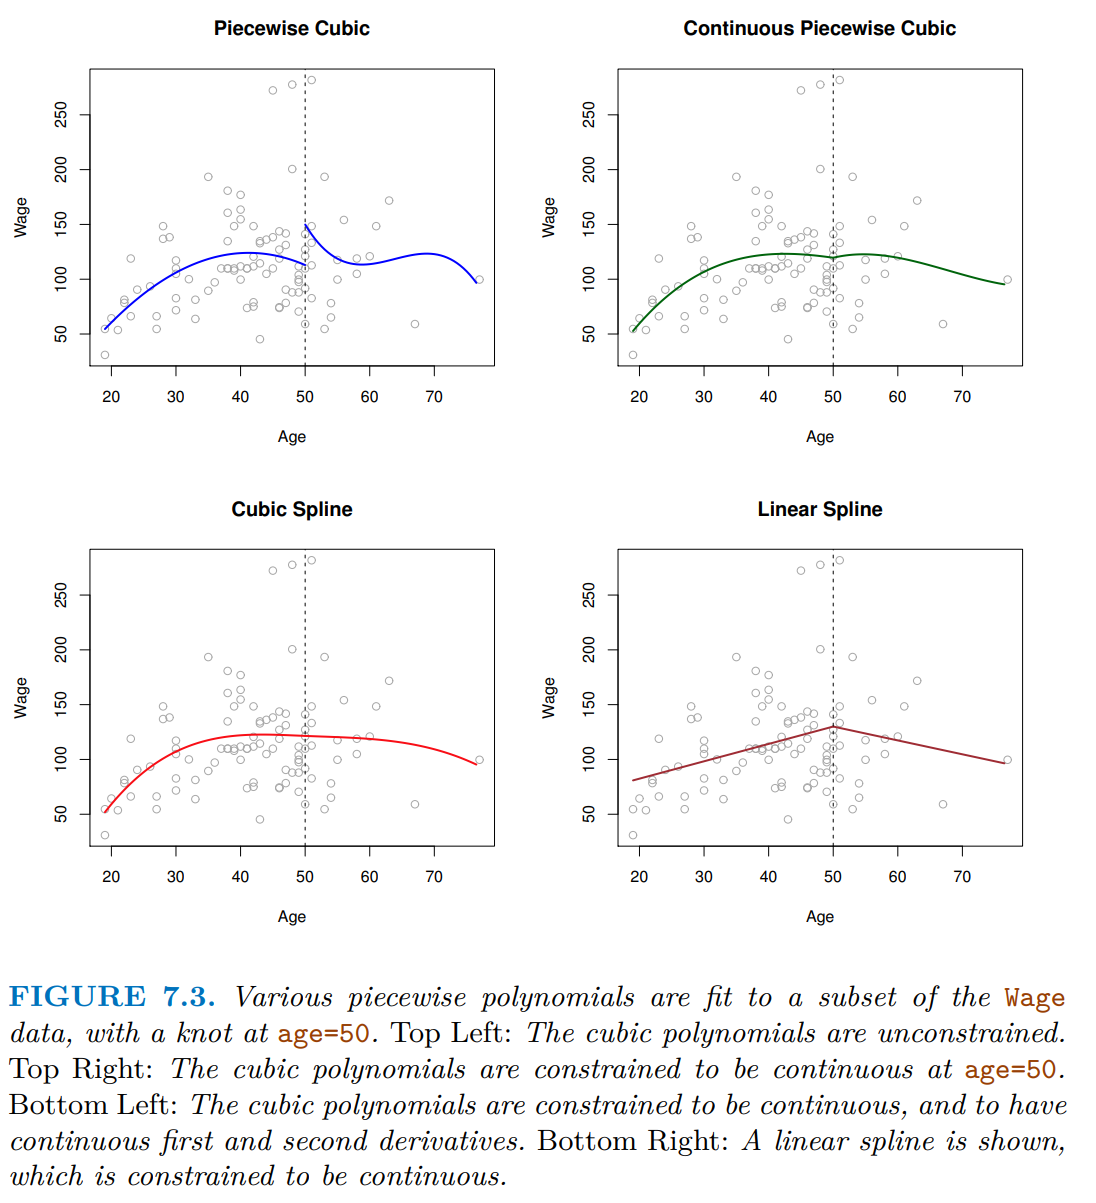
\includegraphics[width=0.8\textwidth]{Regression Splines Visualisations.png}
\end{center}

\subsubsection{Constraints and splines}
\begin{itemize}
    \item The fitted curve must be continuous
    \item The fitted curve should be very smooth
        \begin{itemize}
            \item For cubic spline: the first and second derivatives of the piecewise cubic function need to be continuous at each know
            \item For $d$-degree spline: the continuity in derivatives is required for up to degree $d-1$ at each knot
        \end{itemize}
    \item Each constraint we impose on the piecewise polynomials reduce on degree of freedom
    \item A \textit{natural spline} is a regression spline with linear boundary constraints: the spline function is required to be linear in the region where $X$ is the smaller than the smallest know, or larger than the largest knot
\end{itemize}

\subsubsection{Choosing the number and location of knots}
\begin{enumerate}
    \item Place more knots in places where we feel the function might vary most rapidly (place fewer knots where it seems more stable)
    \item Place knots in a uniform fashion. Firstly, specify the desired degrees of freedom, and then have software place the corresponding number of knots at uniform quantiles of the data.
\end{enumerate} \phantom{i}

\noindent \textbf{CV to choose optimal number of knots}
\begin{enumerate}
    \item Remove a portion of the data (e.g. $10\%$, then fit a spline with a certain number of knots to the remaining data
    \item Use fitted spline to make predictions for the held-out data
    \item Repeat steps 1-2 until each observation has been held-out once, and then compute the overall cross-validated RSS
    \item Repeat steps 1-3 for different number of knots $K$
    \item Value of $K$ that gives the smallest RSS is the optimal one
\end{enumerate} \phantom{i}

\noindent \textbf{Regression splines vs polynomial regression}
\begin{itemize}
    \item To increase flexibility, polynomial regression must use a high degree, while splines can simply increase number of knots but keeping the degree fixed. The latter generally produces more stable estimates
    \item Splines also allow us to adjust the position of the knots to create more flexibility. The polynomial regression doesn't have this feature
\end{itemize}

\subsubsection{Splines in R}
\begin{lstlisting}
library(splines) # used for ns (natural cubic spline)
fit2=lm(wage~ns(age,df=4),data=Wage)
pred2=predict(fit2,newdata=list(age=age.grid),se=T)

# Another way of draw plots with CIs
plot(age,wage,col="gray")
lines(age.grid,pred2$fit,lwd=2)
lines(age.grid,pred2$fit+2*pred2$se,lty="dashed")# Upper bound
lines(age.grid,pred2$fit-2*pred2$se,lty="dashed")# Lower bound

dim(ns(age,df=4)) # df=4 gives three knots for ns()
attr(ns(age,df=4),"knots") # get knots attributes of the matrix ns
\end{lstlisting}

\subsection{Smoothing Splines}
\noindent Find some function $g(x)$ that can fit the observed data well. We need to consider both adherence and smoothness. \\

\noindent Adherence measured by the $RSS = \sum_{i=1}^{n}{(y_i - g(x_i))^2}$, and the smoothness can be measured by $\int g''(t)^2 \ dt$. Since there is a trade-off between adherence and smoothness, we construct the following objective function (with $\lambda \geq 0$): $\sum_{i=1}^{n}(y_i - g(x_i))^2 + \lambda \int g''(t)^2 \ dt$ (like \textit{loss} + \textit{penalty}). \\

\noindent \textbf{Some remarks:}
\begin{itemize}
    \item $\lambda = 0$: smoothness term has no effect. $g$ will be very jumpy and will exactly interpolate the training observations
    \item $\lambda \rightarrow \infty$, $g$ will be perfectly smooth
    \item So $\lambda$ controls the bias-variance trade-off of the smoothing spline
    \item Smoothing spline can be shown to be a nutral cubic spline with knots at the unique values of $x_1,...,x_n$
\end{itemize} \phantom{i}

\noindent \textbf{The effective degrees of freedom}:
\begin{itemize}
    \item $\lambda$ controls the smoothness of the spline, and hence hte effective degrees of freedom
    \item When $\lambda$ increases from $0$ to $\infty$, the effective degrees of freedom, denoted by $df_\lambda$, decrease from $n$ to $2$
    \item $df_\lambda$ is a measure of the flexibility of the smoothing spline
\end{itemize} \phantom{i}

\noindent \textbf{Choosing the smoothing parameter $\lambda$:} Find a value of $\lambda$ that makes the CV RSS as small as possible. LOOCV can also be computed for smoothing splines, using the following formula $RSS_{cv}(\lambda) = \sum_{i=1}^{n}{\Big[ \frac{y_i - \hat{g}_{\lambda}(x_i)}{1 - \{ \boldsymbol{S}_\lambda \}_{ii}} \Big]^2}$, where $\hat{\boldsymbol{g}}_\lambda = \boldsymbol{S}_{\lambda} \boldsymbol{y}$

\subsubsection{Smoothing splines in R}
\begin{lstlisting}
fit=smooth.spline(age,wage,df=16) # lambda determined by df=16
fit2=smooth.spline(age,wage,cv=TRUE) # lambda determined by CV
fit2$df # df under CV

# Plotting example
plot(age,wage,xlim=agelims,cex=.5,col="darkgrey")
title("Smoothing Spline")
lines(fit,col="red",lwd=2)
lines(fit2,col="blue",lwd=2)
legend("topright",legend=c("16 DF","6.8 DF"),col=c("red","blue"),lty=1,lwd=2,cex=.8)
\end{lstlisting}

\subsection{Local Regression}
\noindent Local regression at $X = x_0$:
\begin{enumerate}
    \item Gather the fraction $s=\frac{k}{n}$ of training points whose $x_i$ are closest to $x_0$
    \item Assign a weight $K_{i0} = \omega \cdot \frac{x_i - x_0}{h(x_0)}$ to each point in this neighbourhood, where $h(x_0)$ is the bandwidth, the distance from $x_0$ to its $k$th closest $x_i$
    \item Fit a weighted least squares regression of the $y_i$ on the $x_i$ using the aforementioned weights, by finding $\hat\beta_0$ and $\hat\beta_1$ that minimise $\sum_{i=1}^{n}{K_{i0}(y_i - \beta_0 - \beta_1x_i)^2}$
    \item The fitted value at $x_0$ is given by $\hat{f}(x_0) = \hat\beta_0 + \hat\beta_1 x_0$
\end{enumerate} \phantom{i} \\
\noindent $s$ controls the flexibility of the non-linear fit. The smaller the $s$, the more local and wiggly will be our fit; alternatively, a very large $s$ will lead to a global fit to the data using all of the training observations. CV can be used to choose $s$. \\

\noindent \textbf{Why Local Regression?}
\begin{itemize}
    \item Adapts well to bias problems at boundaries and in regions of high curvature
    \item Easy to understand and interpret
    \item Methods have been developed that provide fast computation for one or more independent variables
    \item Very simple, can be used to work for different distributional assumptions
    \item A local model enables derivation of response adaptive methods for span value and polynomial order selection in a straightforward manner
\end{itemize} \phantom{i}

\noindent \textbf{How to choose polynomial degree?}: The choice is a bias-variance trade off. A higher degree will produce a less biased, but more variable estimate than a lower degree one. \\

\noindent \textbf{How to choose the weight function?} Want to consider a weight function $\omega(u)$ that are peaked at $u=0$ and that decay smoothly to $0$ as $u$ increases. A smooth weight function results in a smoother estimate. We also want a weight function that is nonzero only on a bounded interval, helping with computation speed.

\subsubsection{Local regression in R}
\begin{lstlisting}
fit=loess(wage~age,span=.2,data=Wage) # 20% of the neighborhood
fit2=loess(wage~age,span=.5,data=Wage) # 50% of the neighborhood
# Large span (s) => smoother curve. Span determines the proportion of the data
# used in each localised regression.

# Plotting example 
plot(age,wage,xlim=agelims,cex=.5,col="darkgrey")
title("Local Regression")
lines(age.grid,predict(fit,data.frame(age=age.grid)),col="red",lwd=2)
lines(age.grid,predict(fit2,data.frame(age=age.grid)),col="blue",lwd=2)
legend("topright",legend=c("Span=0.2","Span=0.5"),col=c("red","blue"),lty=1,lwd=2,cex=.8)
\end{lstlisting}

\subsection{Generalised Linear Models (GLMs)}
\begin{itemize}
    \item \textit{Probability distribution}: Instead of assuming normal distribution, GLMs work with distributions in the exponential family (e.g. normal, Poisson, binomial, and gamma)
    \item \textit{Model for the mean}: The mean is a linear function of hte predictors, $\boldsymbol{X}$, $E[Y] = f(\boldsymbol{X})$. In GLMs some smooth monotonic transformation of the mean is a linear function of $\boldsymbol{X}$. $g(E[Y]) = f(\boldsymbol{X})$.
\end{itemize} \phantom{i}

\noindent \textbf{Why GLMs:}
\begin{itemize}
    \item Easy to estimate standard errors, constructing CIs, testing, model selection and other statistical features
    \item GLMs are vary common in many areas of statistics, so they are constantly improving and we can draw upong developments from many industries
    \item There is standard software for fitting GLMs
    \item Although there is standard software companies create their own specialised GLMs so there is space to innovate
\end{itemize} \phantom{i}

\noindent \textbf{The exponential family and the link function:} \\
\noindent GLMs involve distributions that can be expressed in exponential form: $f(y|\theta, \phi) = e^{\frac{y\theta - b(\theta)}{\phi} + c(y,\theta)}$, $\theta$ is the canonical parameter, and $\phi$ is the dispersion parameter (that plays a role in defining the variance of $y$). \\

\noindent The canonical parameter $\theta$ is a function of $\mu$, denoted by $\theta(\mu)$, the canconical link function:
\begin{itemize}
    \item Normal: $\theta(\mu) = \mu$
    \item Poisson: $\theta(\mu) = \ln(\mu)$
    \item Exponential, gamma: $\theta(\mu) = -\mu^-1$
    \item Categorical, binomial, multinomial: $\theta(\mu) = \ln\Big( \frac{\mu}{1-\mu} \Big)$
\end{itemize}

\subsection{Generalised Additive Models (GAMs)}
\noindent GAMs extend multiple linear regression by allowing each variable to have its own non-linear effect, then adding them up:
$$y_i = \beta_0 + f_1(x_{i1}) + f_2(x_{i2}) + ... + f_p(x_{ip}) + \varepsilon_i$$
\noindent Could use and combine any non-linear methods such as local regression, polynomial regression, splines, or any combination of the approaches discussed. Also could use qualitative variables using dummy variables.
\subsubsection{Pros and Cons}
\noindent \textbf{Pros}
\begin{itemize}
    \item GAM allow non-linear $f_j$ to each $X_j$ and does it automatically, so we don't need to manually try out many different transformations.
    \item Non-linear fit could make more accurate predictions.
    \item Since model is additive, we can still examine the effect of each $X_j$ on $Y$ individually while holding all the other variables fixed. Hence GAMs provid useful inference.
    \item Smoothness of function $f_j$ for $X_j$ can be summarised via degrees of freedom.
\end{itemize} \phantom{i}

\noindent \textbf{Cons}
\begin{itemize}
    \item Restricted to be additive. Imporatnt interactions may be missed, however we can add interaction terms to the GAM model by including additional predictors of the form $X_j \times X_k$. In addition we can add low-dimensional interaction functions of the form $f_{jk}(X_j, X_k)$; such terms can be fit using two-dimensional smoothers such as local regression.
\end{itemize}

\subsubsection{GAMs in R}
\noindent \textbf{Using gam library:}
\begin{lstlisting}
library(gam)
gam1=lm(wage~ns(year,4)+ns(age,5)+education,data=Wage) # ns() natural cubic spline
gam.m3=gam(wage~s(year,4)+s(age,5)+education,data=Wage) # s() smoothing splines
par(mfrow=c(1,3))
plot(gam.m3, se=TRUE, col="blue") # same as plot.Gam()
plot.Gam(gam1, se=TRUE, col="red") # upper case plot.Gam for gam library

gam.m1=gam(wage~s(age,5)+education,data=Wage)
gam.m2=gam(wage~year+s(age,5)+education,data=Wage)
anova(gam.m1,gam.m2,gam.m3,test="F")
summary(gam.m3) #only age shows significant non-linearity

# Predictions
preds=predict(gam.m2,newdata=Wage)
mean((preds-Wage$wage)^2) # training MSE
\end{lstlisting}

\noindent \textbf{Logistic regression GAM using gam}
\begin{lstlisting}
gam.lo=gam(wage~s(year,df=4)+lo(age,span=0.7)+education,data=Wage)
plot.Gam(gam.lo, se=TRUE, col="green")
gam.lo.i=gam(wage~lo(year,age,span=0.5)+education,data=Wage)
\end{lstlisting}

\noindent \textbf{Using mgcv library:}
\begin{lstlisting}
library(mgcv)
gam.new=mgcv::gam(wage~year+s(age)+education,data=Wage,method="REML")
summary(gam.new)
plot.gam(gam.new, se=TRUE, col="purple") # lower case plot.gam for mgcv library
\end{lstlisting}

\noindent \textbf{Logistic regression GAM using mgcv}
\begin{lstlisting}
gam.lr=gam(I(wage>250)~year+s(age,df=5)+education,family=binomial,data=Wage)
par(mfrow=c(1,3))
plot(gam.lr,se=T,col="green")
table(education,I(wage>250))
gam.lr.s=gam(I(wage>250)~year+s(age,df=5)+education,
    family=binomial,data=Wage,subset=(education!="1. < HS Grad"))
plot(gam.lr.s,se=T,col="green")
\end{lstlisting}

\newpage
\section{Logistic Regression and Bayes Theorem}

However, the key new topic in Week 6 was \textbf{Logistic Regression}, a classification method.

\subsection{Classification Methods (Introduction)}
Types:
\begin{enumerate}
    \item Logistic regression
    \item Linear discriminant analysis (LDA)
    \item Quadratic discriminant analysis (QDA)
    \item Naive Bayes
    \item K-nearest neighbours
    \item Classification trees
    \item Support vector machines
\end{enumerate}
\vspace{1em} \noindent Used to capture a qualitative variable instead of a quantitative one. Why can't we encode a variable using linear regression past a binary response? (a) A regression method cannot accommodate a qualitative response with more than two classes (as order of the classes matters and how different they are to each other matters in regression), (b) A regression method will not provide meaningful estimates of $Pr(Y|X)$, even with just two classes.


\subsection{Logistic Regression Theory}
For a binary outcome $Y$ (two classes, often coded as 0/1 for convenience), logistic regression models the \textbf{probability} of $Y=1$ as a function of predictors $X$. We write:
\[ p(X) = P(Y=1 \mid X) = \frac{\exp(\beta_0 + \beta_1 X_1 + \cdots + \beta_p X_p)}{1 + \exp(\beta_0 + \beta_1 X_1 + \cdots + \beta_p X_p)}. \]
This is the \textbf{logistic function} mapping $\mathbb{R}$ to $(0,1)$. It ensures predicted probabilities stay between 0 and 1, unlike a linear model. \\

\noindent The logistic model: $p(X) = \frac{e^{\beta_{0}  + \beta_{1}X}}{1 + e^{\beta_{0} + \beta_{1}X}}$ and the multiple logistic regression: $p(\boldsymbol{X}) = \frac{e^{\beta_{0} + \beta_{1}X_{1} + ... + \beta_{p}X_{p}}}{1 + e^{\beta_{0} + \beta_{1}X_{1} + ... + \beta_{p}X_{p}}}$ \\

\noindent Taking odds:
\[ \frac{p(X)}{1-p(X)} = \exp(\beta_0 + \beta_1 X_1 + \cdots + \beta_p X_p) \in (0, \infty), \]
If odds close to $0 \implies $ very low probability of $X$ and odds close to $\infty \implies$ very high probability of $X$. \\
\noindent So the \textbf{log-odds} (logit) is linear:
\[ \log\frac{p(X)}{1-p(X)} = \beta_0 + \beta_1 X_1 + \cdots + \beta_p X_p. \]

\noindent Interpretation: $\beta_j$ now is the change in log-odds for a one unit increase in $X_j$, holding others fixed. Equivalently, $e^{\beta_j}$ is the multiplicative change in the odds for a one-unit increase in $X_j$. For example, if $\beta_j = 0.7$, then odds are $e^{0.7}\approx2.01$ times greater for a one-unit increase in $X_j$ (meaning $p$ roughly doubles, if in mid-range).

\noindent Logistic regression is fit by \textbf{maximum likelihood} rather than least squares (since it's not a linear model in $Y$). The likelihood for independent observations is 
\[ L(\beta_0,\boldsymbol{\beta}) = \prod_{i: y_i=1} p(x_i) \prod_{j: y_j=0} [1-p(x_j)], \]
and we find $\hat\beta$ that maximize this (often via iterative algorithms).  \\

\noindent The output in R often includes:
\begin{itemize}
    \item Coefficients (values of $\beta_j$), measures relationship of each predictor with the response
    \item Standard error (SE$(\beta_j)$)
    \item $z$-statistics ($\frac{\hat{\beta}_j}{\text{SE}(\hat{\beta}_j)}$)
    \begin{itemize}
        \item A large (absolute) value of the $z$-statistic indicates evidence against the null hypothesis $H_0: \; B_j = 0$ (meaning there is a meaningful relationship between the predictor $X_j$ and $Y$)
    \end{itemize}
    \item P-values. If $p$ is tiny, we can reject $H_0 \implies$ there is a meaningful relationship between $X_j$ and $Y$
\end{itemize} 
\phantom{i}
\\ \noindent We measure model fit by \textbf{deviance} or by classification performance metrics, since $R^2$ isn't meaningful here. One can compute a pseudo-$R^2$ or just measure accuracy. \\

\noindent \textbf{Prediction rule:} To make a classification, we predict class 1 if $\hat p(X) > 0.5$ (or another cutoff). 0.5 is the default threshold for equal costs. Sometimes we adjust the threshold for specific sensitivity or specificity needs (e.g., predict positive if probability $>$ 0.2 to catch more positives at cost of more false alarms, as shown by altering threshold in slides for LDA; similar logic applies to logistic). \\

\noindent \textbf{Making predictions:} Once you have coefficients, we can compute the probability of event $X$ (use probability of default as the example). E.g. if credit card balance $X = \$1,000$, $\hat{p}(X) = \frac{e^{\hat{\beta}_{0} + \hat{\beta}_{1}X}}{1 + e^{\hat{\beta}_{0} + \hat{\beta}_{1}X}} = \frac{e^{-10.6513 + 0.0055 \times 1000}}{1 + e^{-10.6513 + 0.0055 \times 1000}} = 0.00576$ \\

\noindent \textbf{Qualitative predictors (dummy variable encoding):} Can fit a model and the predictor can be $0$ if some condition is satisfied, and $1$ if not, then can fit a simple logistic model based on that. \\

\noindent \textbf{Pros:}
\begin{itemize}
    \item  Outputs probabilities, which is more informative than just class labels (especially in insurance, you might use the probabilities for decision).
    \item Well-calibrated (if model is correct, predicted probabilities tend to reflect true frequencies).
    \item Inference is available (Wald tests via $z$-values).
    \item Can naturally extend to multiple classes (via multinomial logistic, not covered deeply but concept exists).
\end{itemize}


\noindent \textbf{Cons:}
\begin{itemize}
    \item Assumes a linear log-odds relationship. If the true decision boundary is highly non-linear, logistic (without polynomial terms or interactions) will mis-specify.
    \item It’s parametric; if parametric form is wrong, could be biased.
    \item In practice, if classes are not well separated, parameter estimates have large uncertainty (though still optimal in max likelihood sense).
\end{itemize}

\subsection{Logistic Regression in R}
\begin{lstlisting}
library(ISLR)
?Smarket # info on dataset used

# Fitting a logistic regression (no test/train set)
glm.fits=glm(Direction~Lag1+Lag2+Lag3+Lag4+Lag5+Volume,
             data=Smarket,family=binomial) # binomial for LR
summary(glm.fits)
#  Coefficients:
#               Estimate Std. Error z value Pr(>|z|)
#  (Intercept) -0.126000   0.240736  -0.523    0.601
# Lag1        -0.073074   0.050167  -1.457    0.145
# Lag2        -0.042301   0.050086  -0.845    0.398
# Lag3         0.011085   0.049939   0.222    0.824
# Lag4         0.009359   0.049974   0.187    0.851
# Lag5         0.010313   0.049511   0.208    0.835
# Volume       0.135441   0.158360   0.855    0.392
# (Dispersion parameter for binomial family taken to be 1)
#    Null deviance: 1731.2  on 1249  degrees of freedom
#  Residual deviance: 1727.6  on 1243  degrees of freedom
# AIC: 1741.6
# Number of Fisher Scoring iterations: 3
coef(glm.fits)
summary(glm.fits)$coef
summary(glm.fits)$coef[,4] # Showing the associated p-values only
glm.probs=predict(glm.fits,type="response") # type="response" returns P(Y=1|X)
contrasts(Direction)
glm.pred=rep("Down",1250) # creating 1250 Down elements
glm.pred[glm.probs>.5]="Up" # transforming those elements whose prob.>0.5 to Up
table(glm.pred,Direction) # The confusion matrix
mean(glm.pred==Direction) # rate of correct predictions, i.e. 1-training error rate
mean(glm.pred!=Direction) # training error rate

# Fit the logistic regression using training set
train=(Year<2005)
Smarket.2005=Smarket[!train,] # selecting observations in 2005
dim(Smarket.2005)
Direction.2005=Direction[!train]
glm.fits=glm(Direction~Lag1+Lag2+Lag3+Lag4+Lag5+Volume,
             data=Smarket,family=binomial,subset=train) # subset=train for train data only
# Predict using test set
glm.probs=predict(glm.fits,Smarket.2005,type="response")
glm.pred=rep("Down",252)
glm.pred[glm.probs>.5]="Up"
table(glm.pred,Direction.2005)
mean(glm.pred==Direction.2005) #rate of correct predictions
mean(glm.pred!=Direction.2005) #test error rate
sum(glm.pred==Direction.2005 & glm.pred=="Down")
#Sensitivity
sum(glm.pred==Direction.2005 & glm.pred=="Up")/sum(Direction.2005=="Up")

# model improvement by removing weakest predictors
glm.fits=glm(Direction~Lag1+Lag2,data=Smarket,family=binomial,subset=train)
glm.probs=predict(glm.fits,Smarket.2005,type="response")
glm.pred=rep("Down",252)
glm.pred[glm.probs>.5]="Up"
table(glm.pred,Direction.2005)
mean(glm.pred==Direction.2005)
#Sensitivity
sum(glm.pred==Direction.2005 & glm.pred=="Up")/sum(Direction.2005=="Up")
# predict using new observations x1=(1.2, 1.1) and x2=(1.5, -0.8)
predict(glm.fits,newdata=data.frame(Lag1=c(1.2,1.1),Lag2=c(1.5,-0.8)),type="response")
\end{lstlisting}

\subsection{Bayes' theorem for classification:}
\noindent Suppose we wish to classify an observation into one of $K$ classes ($K \geq 2$). \\

\noindent Let $\pi_{k}$ denote the overall or \textit{prior} probability that a randomly chosen observation comes from class $k$. \\

\noindent Let $f_k(x) = \mathbb{P}(X=x|Y=k)$ be the density function of $X$ for an observation that comes from the $k$th class:
\begin{itemize}
    \item $f_k(x)$ is relatively large if there is a high prob. that an observation in the $k$th class $X \approx x$;
    \item $f_k(x)$ is relatively small if it is unlikely that an observation in the $k$th class has $X \approx x$.
\end{itemize}
\phantom{i}
\\ \noindent Then Bayes' theorem states that:
$$p_k(x) = \mathbb{P}(Y=k|X=x) = \frac{\pi_k f_k(x)}{\sum_{I=1}^{K}{\pi_I f_I(x)}}$$
\noindent We can estimate $\pi_k$ and $f_k(x)$ seperately and then plug in those estimatees into the equation above to obtain an estimate of $p_k(x)$. \textit{LDA}, \textit{QDA} and \textit{naive Bayes} all use different estimates of $f_k(x)$.

\newpage    
\section{Linear/Quadratic Discriminant Analysis and KNN}
\subsection{LDA Theory}

\subsubsection{LDA for $p = 1$:}
\noindent We only have $1$ predictor, $f_k(x) = \frac{1}{\sqrt{2\pi}\sigma_{k}}e^{-\frac{(x-\mu_k)^2}{2\sigma_{k}^{2}}}$, assume that $\sigma_1^2 = ... = \sigma_k^2 = \sigma^2$. Therefore:

$$p_k(x) = \frac{\pi_k e^{-\frac{(x - \mu_k)^2}{2\sigma^2}}}{\sum_{I=1}^{K}{\pi_I  e^{-\frac{(x - \mu_k)^2}{2\sigma^2}}}}$$

\noindent \textbf{How to classify an observation $\boldsymbol{X = x}$}: We take $\delta_k(x) = \ln(p_k(x))$ and try to maximise it. Re-arrange terms to get $\delta_k(x) = x \cdot \frac{\mu_k}{\sigma^2} - \frac{\mu_k^2}{2\sigma^2} + \log(\pi_k)$. \\

\noindent E.g. If $K=2$ and $\pi_1 = 0.5$. Find the condition that $x$ needs to satisfy such that the Bayes classifier assigns observation $X=x$ to class $1$: \\

\begin{align*}
    \text{For } & \mu_1 > \mu_2: \\
    \delta_1(x) > \delta_{2}(x) &\Leftrightarrow x(\mu_1 - \mu_2) - \frac{1}{2}(\mu_1^2 - \mu_2^2) > 0 \\
    &\Leftrightarrow x > \frac{\mu_1 + \mu_2}{2} \Leftrightarrow Y = 1
\end{align*}

\noindent Clearly, if $\mu_1 < \mu_2$, then $x < \frac{\mu_1 + \mu_2}{2}$. The point $x = \frac{\mu_1 + \mu_2}{2}$ is the Bayes decision boundary. \\

\noindent \textbf{Estimations used in LDA:} LDA estimates parameters then plugs them into $\delta_k(x)$. Assume $n$ is the total \#observations in the training data set, and $n_k$ is the number of training observations in the $k$th class. \\

\begin{align*}
    \hat{\mu}_k &= \frac{1}{n_k} \sum_{i: y_i = k}{x_k} \\
    \hat{\sigma}^2 &= \frac{1}{n-K}\sum_{k=1}^{K}\sum_{i: y_i = k}(x_i - \hat{\mu_k})^2 \\
    \hat{\pi}_k &= \frac{n_k}{n} \\
    \implies \hat{\delta}_k(x) &= x \cdot \frac{\hat{\mu}_k}{\hat{\sigma}^2} - \frac{\hat{\mu}_k^2}{2\hat{\sigma}^2} + \log(\hat{\pi}_k), \ \text{linear discriminant function of $x$}
\end{align*}

\noindent \textit{The LDA classifier results from assuming that the observations within each class come from a normal distribution with a class-specific mean vector and common variance $\sigma^2$}.

\subsubsection{LDA for $p > 1$:}
\noindent We have $p$-predictors, let $\boldsymbol{X} \sim N(\boldsymbol{\mu}, \boldsymbol{\Sigma})$, Cov($\boldsymbol{X}$) = $\boldsymbol{\Sigma}$, $\implies$ the pdf:
$$f(\boldsymbol{x}) = \frac{1}{(2\pi)^{p/2}\sqrt{|\boldsymbol{\Sigma}|}}e^{-\frac{1}{2}(\boldsymbol{x} - \boldsymbol{\mu})\boldsymbol{\Sigma}^2(\boldsymbol{x} - \boldsymbol{\mu})^\top}$$
$$\delta_k(\boldsymbol{x}) = \boldsymbol{x}\boldsymbol{\Sigma}^{-1}\boldsymbol{\mu}_k^\top - \frac{1}{2}\boldsymbol{\mu}_k^{\top} + \log(\pi_k)$$

\noindent Then we can estimate the unknown parameters like before, to classify a new observation $\boldsymbol{X} = \boldsymbol{x}$, LDA plugs these estimates into $\delta_k(\boldsymbol{x})$ and classifies to the class with the largest $\delta_k(\boldsymbol{x})$. \\

\noindent \textbf{A binary classification problem example:} $10,000$ observations in \textit{Default} training data set, where $333$ individuals defaulted. Perform LDA on the training data and the training error rate is $2.75\%$, some remarks:
\begin{itemize}
    \item The training error rate being low doesn't mean the test error will be low as well, over fitting is a potential issue, in particular when $p$ is close to $n$.
    \item Since only $3.33\%$ of individuals in training data defaulted, the \textit{null} classifier, which always predicts no defaulting, will achieve an training error rate of $3.33\%$, not much higher than the LDA training error rate.
    \item  What does the credit card company really care about?
\end{itemize}
\phantom{i} \\
\noindent Confusion matrix:
\begin{center}
  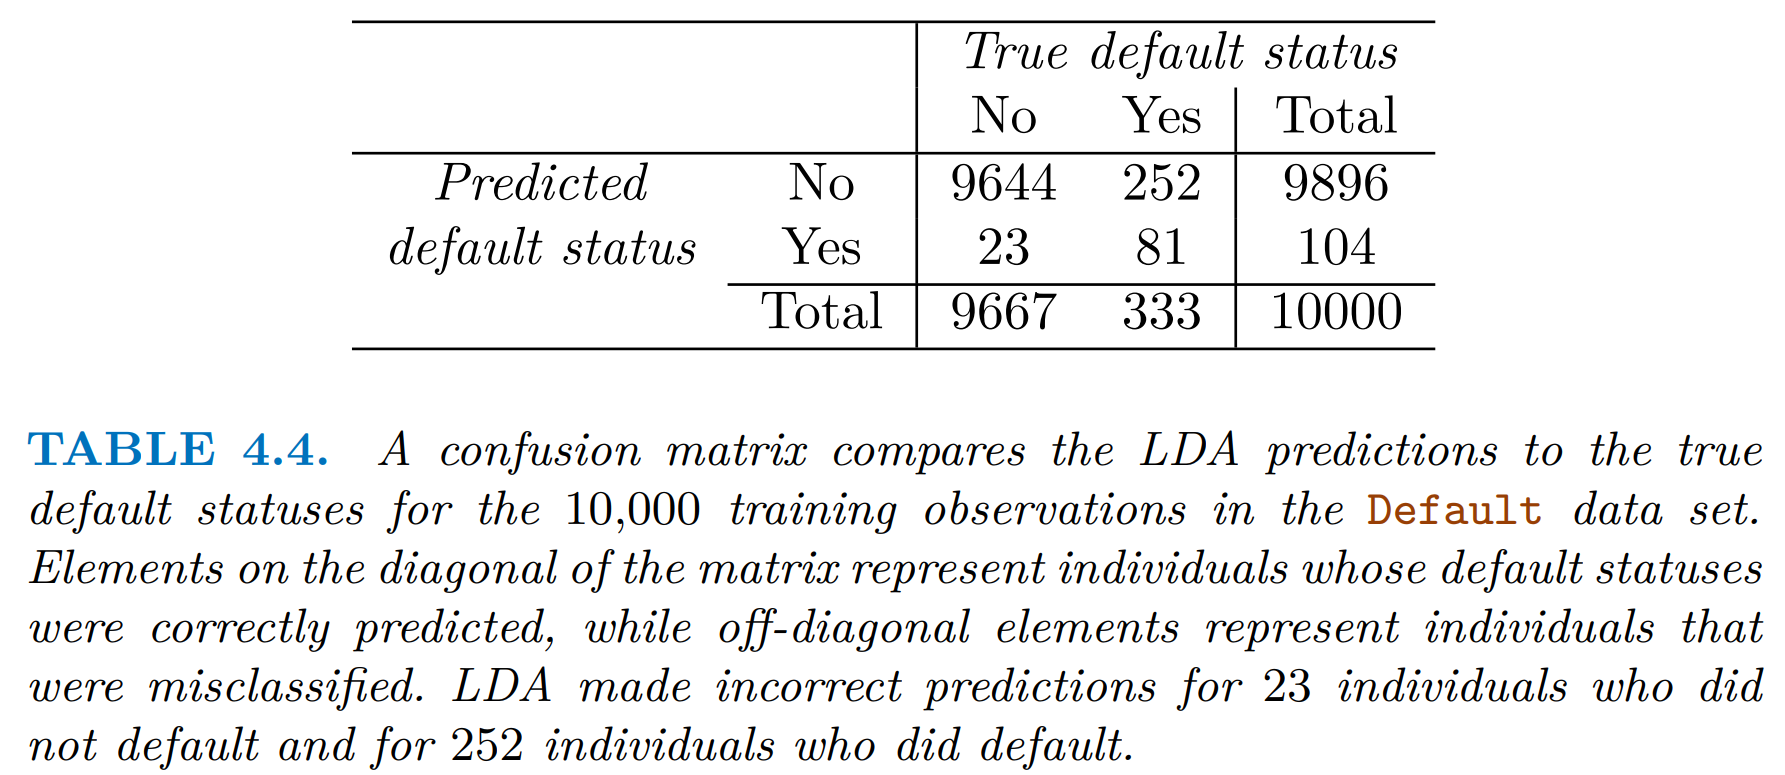
\includegraphics[width=0.8\textwidth]{LDA Example Confusion Matrix.png}
\end{center}

\begin{itemize}
    \item Training error rate is $(252+23)/10000 = 2.75\%$.
    \item Assigning not defaulted individuals to \textit{default} error: $23/9667 = 0.24\%$.
    \item Assigning defaulted individuals to \textit{no default} error: $252/333 = 75.7\%$.
\end{itemize}
\phantom{i} \\
\noindent Is the LDA classifier a satisfactory one?
\begin{itemize}
    \item \textit{Sensitivity} of the LDA classifier: $81/333 = 24.3\%$; very poor!
    \item \textit{Specificity} of the LDA classifer: $9664/9667 = 99.8\%$; Great!
    \item Poor sensitivity so not a satisfactory classifier, since credit card company would usually care more about not incorrectly classifying an individual who will default as no default.
\end{itemize}
\phantom{i} \\
\noindent Can we modify the LDA to better meet the credit card company's need?
\begin{itemize}
    \item Yes. We can modify the threshold used in the LDA approach to achieve the goal. The default threshold is $0.5$, i.e. we assign an observation to the \textit{default} class if $\mathbb{P}(\text{default} = \text{Yes}|\boldsymbol{X} = \boldsymbol{x}) > 0.5$.
    \item If threshold is now $20\%$ sensitivity is better, specificity is still great which is really good although the overall error rate increases a little bit.
\end{itemize}
\phantom{i} \\
\noindent \textbf{Threshold vs. Error Rate Curve:}
\begin{center}
  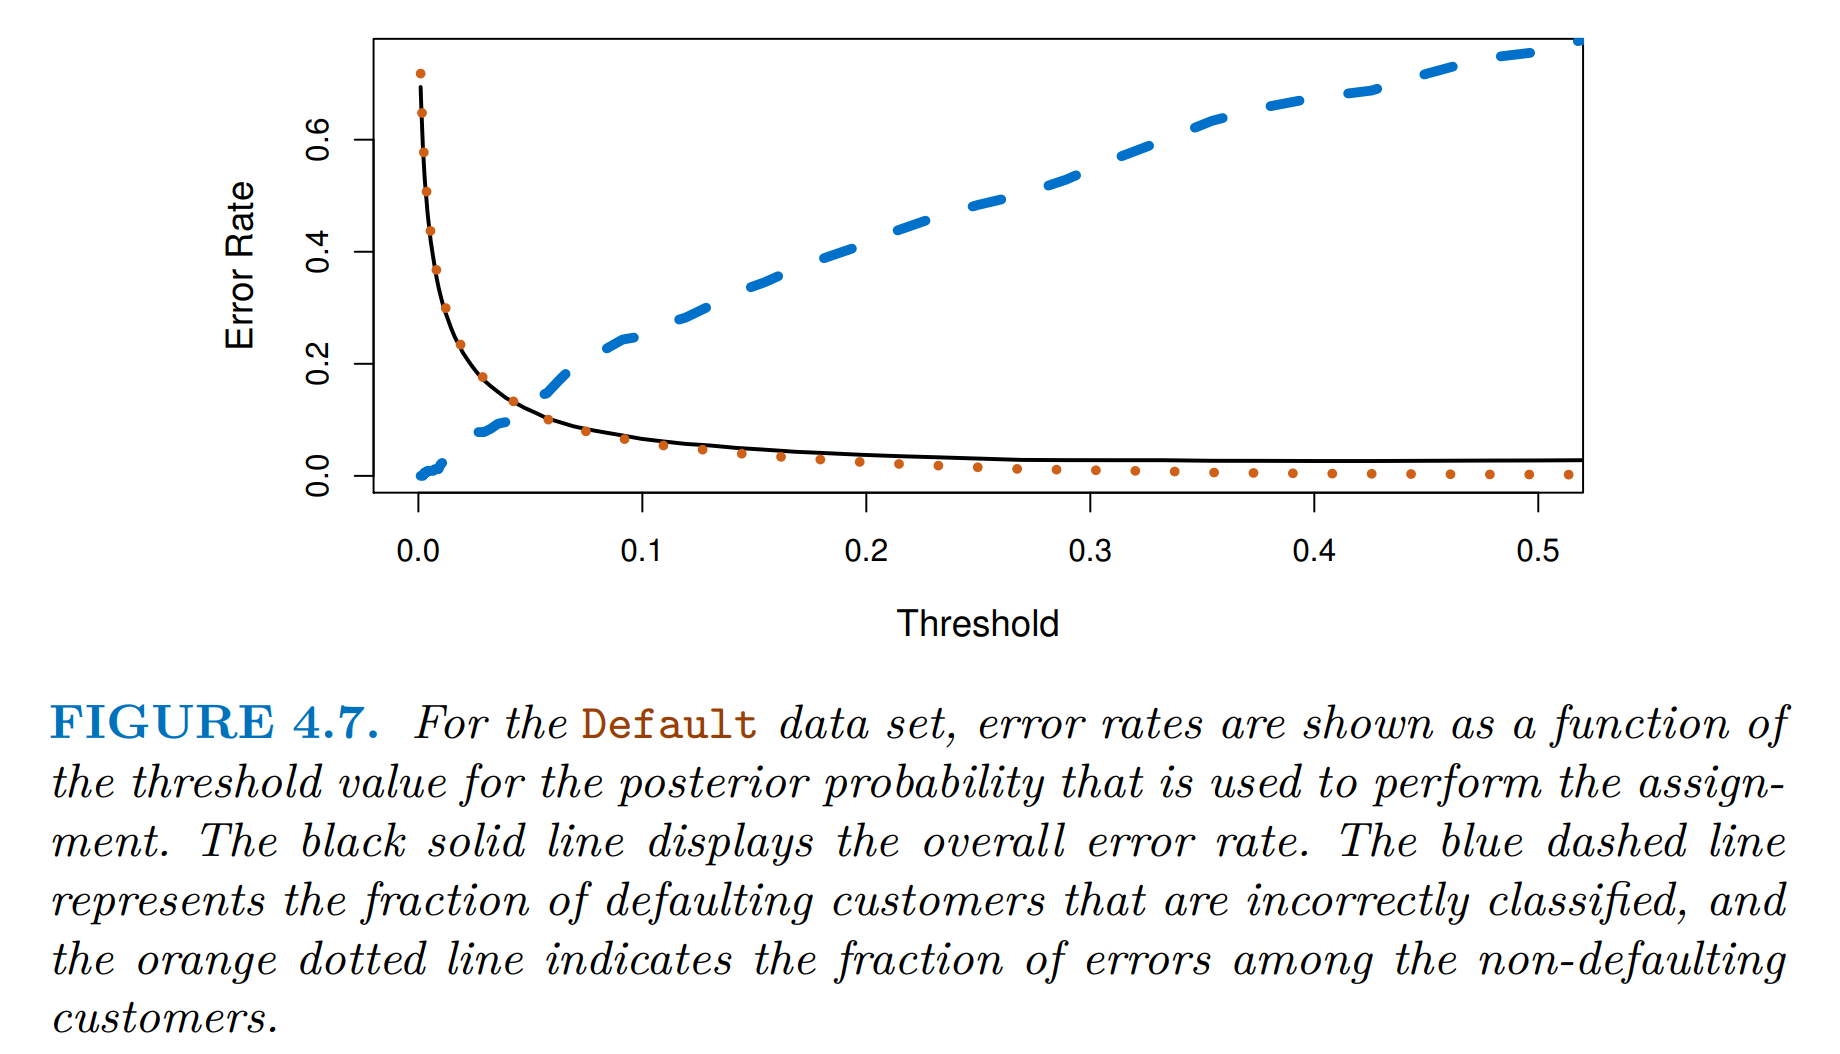
\includegraphics[width=0.8\textwidth]{LDA Example Threshold vs Error Rate.png}
\end{center}
\vspace{7em}
\noindent \textbf{ROC (Receiver Operating Characteristics) Curve:} \\
\noindent How to read: the overall performance of a classifier, summarised over all possible thresholds, is given by the \textit{area under the (ROC) curve} (AUC). An ideal ROC curve will hug the top left corner, so the larger the AUC the better the classifier. \\

\noindent It plots the true positive rate against the false positive rate at various threshold settings associated with the classification algorithm.
\begin{center}
  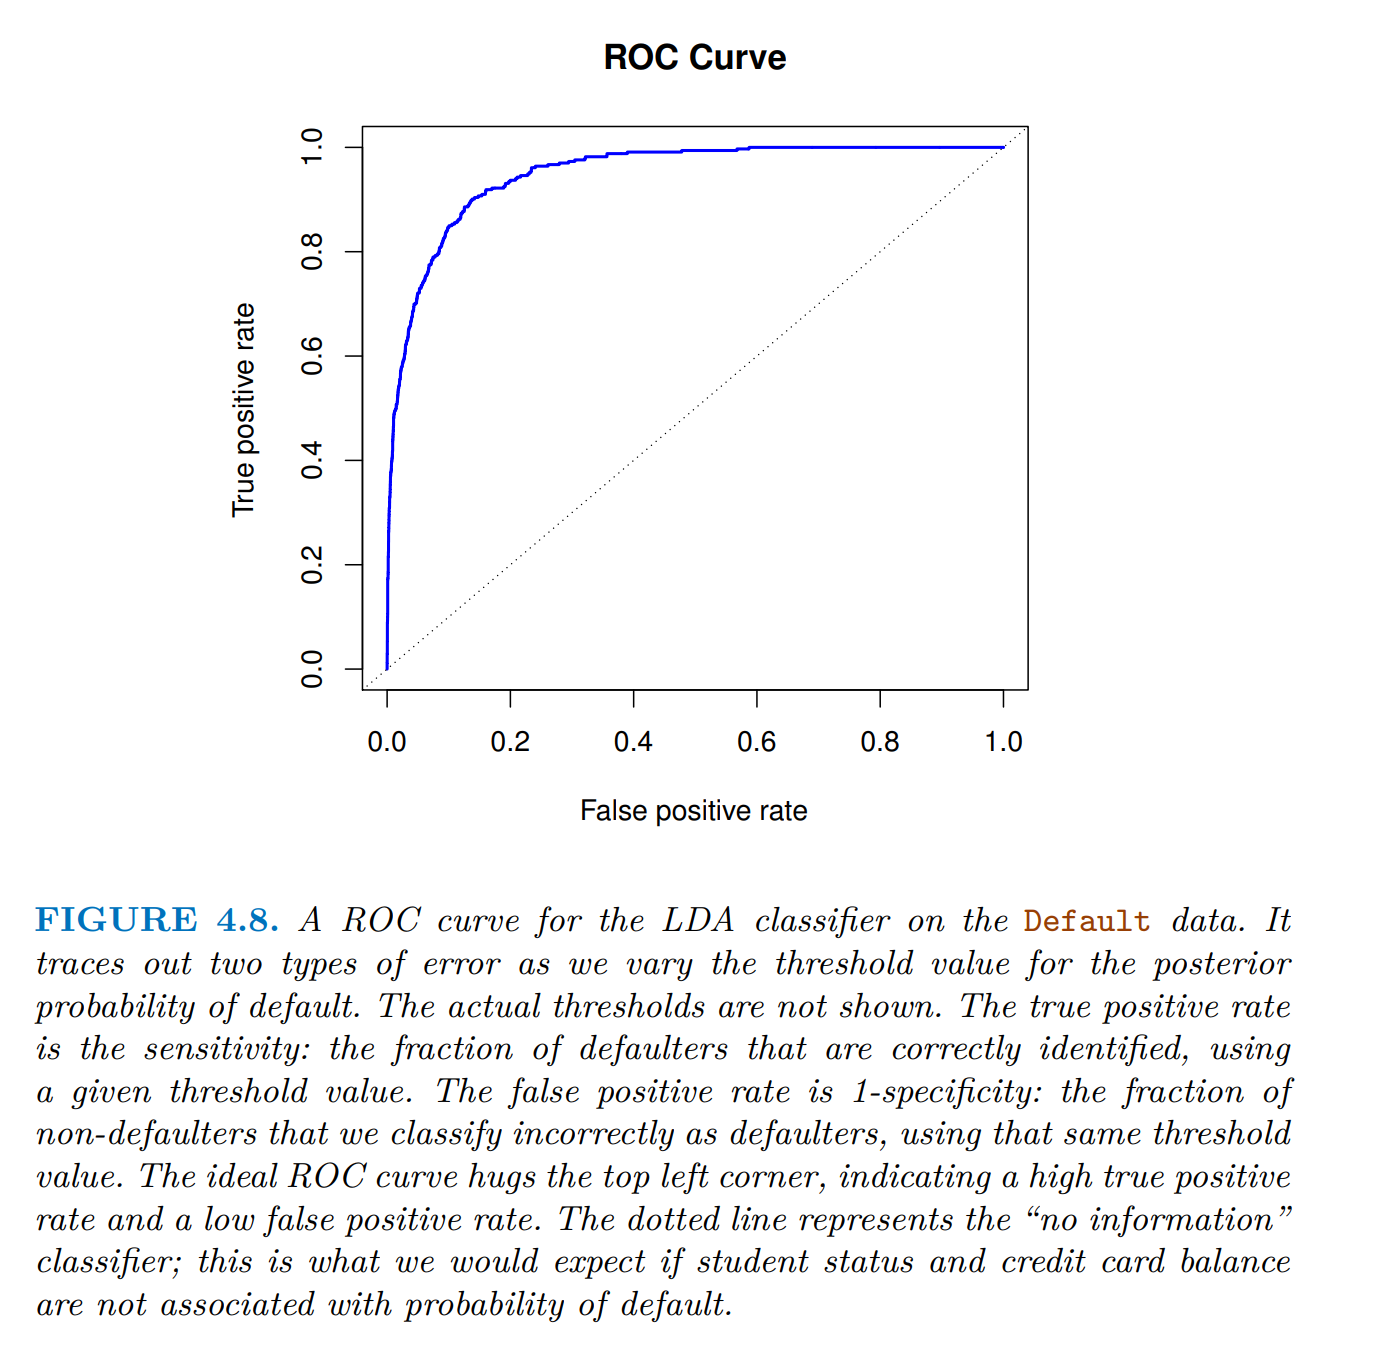
\includegraphics[width=0.8\textwidth]{LDA Example ROC Curve.png}
\end{center}
\phantom{i}\\

\subsection{Confusion Matrices and Measures for Classification}

\begin{center}
  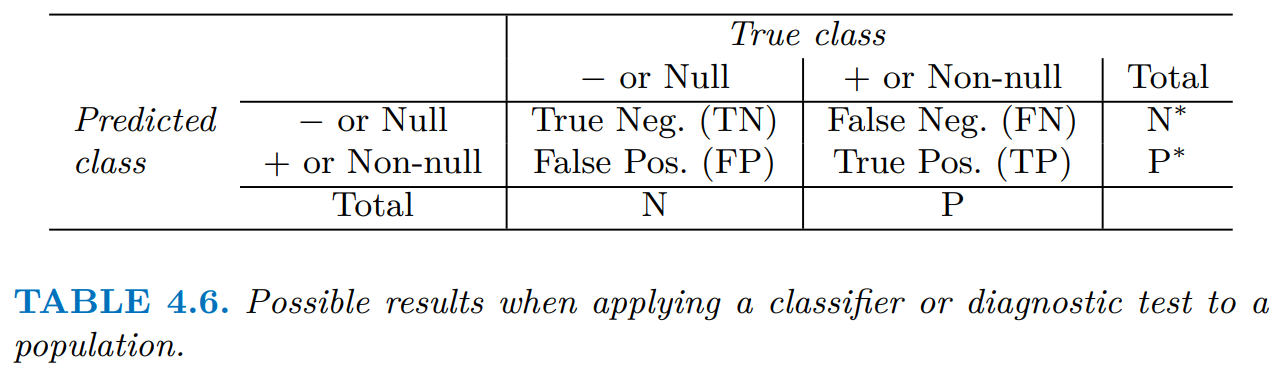
\includegraphics[width=0.8\textwidth]{Classificaiton Confusion Matrix Definition.png}
\end{center}

\begin{center}
  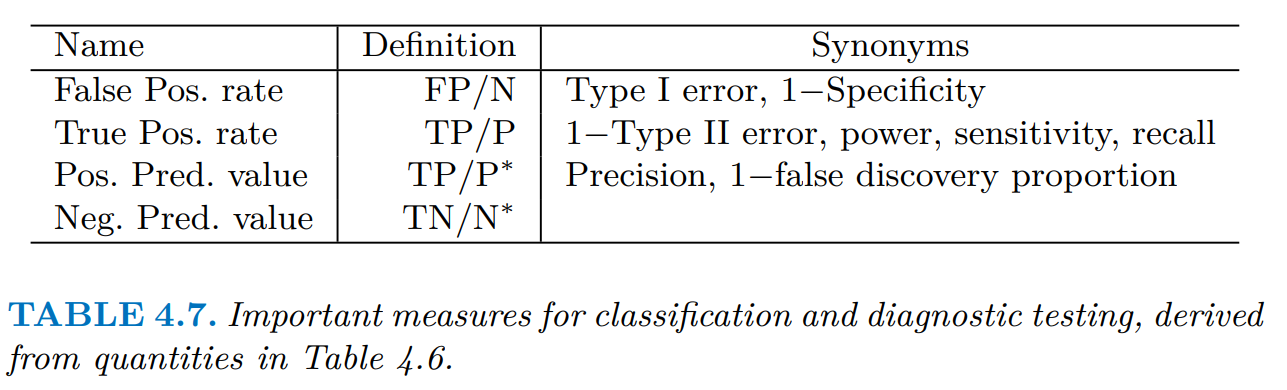
\includegraphics[width=0.8\textwidth]{Measures of Classification.png}
\end{center}

\subsection{Quadratic Discriminant Analysis (QDA):}
Assumes that an observation from the $k$th class is one of the form $\boldsymbol{X} \sim N(\boldsymbol{\mu}_k, \boldsymbol{\Sigma}_k)$, so unique covariance matrices for each class. Therefore we can derive:
\begin{align*}
    \delta_{x}(\boldsymbol{x}) &= -\frac{1}{2}(\boldsymbol{x} - \boldsymbol{\mu}_k)\boldsymbol{\Sigma}_{k}^{-1}(\boldsymbol{x - \boldsymbol{\mu}_k})^\top - \frac{1}{2}\log|\boldsymbol{\Sigma}_k| + \log(\pi_k) \\
    &= -\frac{1}{2}\boldsymbol{x}\boldsymbol{\Sigma}_k^{-1}\boldsymbol{x}^\top + \boldsymbol{x}\boldsymbol{\Sigma}_{k}^{-1}\boldsymbol{\mu}_{k}^{\top} - \frac{1}{2}\boldsymbol{\mu}_k\boldsymbol{\Sigma}_k^{-1}\boldsymbol{\mu}_k^{\top} - \frac{1}{2}\log|\boldsymbol{\Sigma}_k| + \log(\pi_k)
\end{align*}

\noindent Then we plug in estimates for $\boldsymbol{\Sigma}_k$ and $\boldsymbol{\mu}_k$ to assign an observation to the class for which this quantity is the largest, $\boldsymbol{x}$ appears as a quadratic function in the equation above so that's why its a QDA.

\subsubsection{When to use QDA or LDA?}
\noindent The answer depends on the bias-variance trade-off:
\begin{itemize}
    \item LDA is much less flexible classifier than QDA, which lead to lower variance. Since, for $p$ predictors, QDA estimates $K\frac{p(p+1)}{2}$ params. and LDA estaimtes $\frac{p(p+1)}{2}$ params.
    \item If LDA's assumption on common covariance matrix is not appropriate, then it will result in higher bias
    \item LDA tends to be a better bet than QDA if there are relatively fewer training observations and so reducing variance is crucial.
    \item QDA is recommended if the training set is very large, or if the assumption of common covariance matrix for the $K$ classes is clearly untenable (not that great).
\end{itemize}

\subsection{LDA in R}
\begin{lstlisting}
library(ISLR)
attach(Smarket)
train=(Year<2005)
Smarket.2005=Smarket[!train,] #selecting observations in 2005
Direction.2005=Direction[!train]

library(MASS)
lda.fit=lda(Direction~Lag1+Lag2,data=Smarket,subset=train)
lda.fit
# Call:
# lda(Direction ~ Lag1 + Lag2, data = Smarket, subset = train)
# Prior probabilities of groups:
#     Down       Up 
# 0.491984 0.508016 
# Group means:
#             Lag1        Lag2
# Down  0.04279022  0.03389409
# Up   -0.03954635 -0.03132544
# Coefficients of linear discriminants:
#             LD1
# Lag1 -0.6420190
# Lag2 -0.5135293
plot(lda.fit)
lda.pred=predict(lda.fit, Smarket.2005)
names(lda.pred) # "class", "posterior", "x"
lda.pred$posterior[1:10,] #estimated posterior probabilities
lda.pred$class[1:10] #class predictions
lda.class=lda.pred$class
confusion <- table(lda.class,Direction.2005) # Confusion matrix
mean(lda.class==Direction.2005) # True rate
(confusion[1,1]+confusion[2,2])/length(lda.class) # Manual true rate
#recreate predictions using a threshold 0.5
sum(lda.pred$posterior[,1]>=0.5) # Pr(y=down|x)>=0.5
sum(lda.pred$posterior[,1]<.5) # Pr(y=down|x)<0.5
#change threshold
sum(lda.pred$posterior[,1]>0.49)
\end{lstlisting}

\subsection{QDA in R}
\begin{lstlisting}
par(mfrow=c(2,1))
hist(Lag1)
hist(Lag2)
par(mfrow=c(1,1))
qda.fit=qda(Direction~Lag1+Lag2,data=Smarket,subset=train)
qda.fit
# Call:
# qda(Direction ~ Lag1 + Lag2, data = Smarket, subset = train)
# Prior probabilities of groups:
#     Down       Up 
# 0.491984 0.508016 
# Group means:
#             Lag1        Lag2
# Down  0.04279022  0.03389409
# Up   -0.03954635 -0.03132544
qda.class=predict(qda.fit,Smarket.2005)$class # predict then get the classes
table(qda.class,Direction.2005) # Confusion matrix
mean(qda.class==Direction.2005) # True rate
\end{lstlisting}

\subsection{K-Nearest Neighbors (KNN) Theory}
KNN is a non-parametric classification method:
To predict class for an observation $x_0$, find the $K$ training observations closest to $x_0$ (in Euclidean distance, typically). Then have them vote (majority class among those $K$ neighbors). The estimated probability for class $j$ is the fraction of the $K$ neighbors that belong to class $j$:
\[ \Pr(Y=j|X=x_0) = \frac{1}{K} \sum_{i \in N_0} I(y_i = j), \] 
where $N_0$ is the index set of the $K$ nearest neighbors of $x_0$. Then assign the class with highest estimated probability.

\subsubsection{Choosing a K Value}
\begin{itemize}
    \item KNN is very flexible: as $K \to n$, it becomes very smooth (predict majority of entire training set = always most frequent class, high bias, low variance).
    \item As $K \to 1$, it can get very wiggly (each point is basically its own neighborhood, can overfit noise, low bias, high variance).
    \item We choose $K$ by cross-validation typically.
\end{itemize}

\subsubsection{Pros an cons of KNN approach}
\begin{itemize}
    \item \textbf{Pros:}
        \begin{enumerate}
            \item The algorithm is simple and easy to implement.
            \item There is no need to build a model, tune several parameters, or make additional assumptions (like shape of decision boundary).
            \item The algorithm is versatile. It can be used for classification and regression.
            \item Effective if $n$ is very large (lots of data) and relationship is hard to parametric form.
        \end{enumerate}
    \item \textbf{Cons:}
        \begin{enumerate}
            \item No explicit model, so no interpretability beyond "these neighbors vote".
            \item Doesn’t give confidence intervals or the like, though one can derive some asymptotic analysis if needed.
            \item Slow if $n$ is large (need to compute distances to all points for each prediction, though can use indexing structures to speed up).
            \item Curse of dimensionality. KNN works poorly if $p$ is large, because distance in high dimension becomes less meaningful (all points become far). Requires feature scaling or selection and often needs a lot of data.
        \end{enumerate}
\end{itemize}

\subsection{KNN in R}
\begin{lstlisting}
library(class) # library for KNN
train.X=cbind(Lag1,Lag2)[train,]
test.X=cbind(Lag1,Lag2)[!train,]
train.Direction=Direction[train] # get class of train data (in Smarket)
set.seed(5) # ties as nearest neighbors will be randomly broken
knn.pred=knn(train.X,test.X,train.Direction,k=58) # use k=58
table(knn.pred,Direction.2005) # Confusion matrix
mean(knn.pred==Direction.2005) # True rate

knn.rp = rep(0, 101) # test a bunch of k's
for(i in 1:101){
  set.seed(5)
  knn.pred=knn(train.X,test.X,train.Direction,k=i)
  knn.rp[i]=mean(knn.pred==Direction.2005)
}
which.max(knn.rp) # k=58 is the best (highest true rate)

# how to use knn.cv() to select best K
knn.rp = rep(0, 101)
for(i in 1:101){
  set.seed(5)
  knn.pred.cv=knn.cv(train.X,train.Direction,k=i,p=1) # Leave-p-out CV
  knn.rp[i]=mean(knn.pred.cv==train.Direction)
}
k.cv=which.max(knn.rp) # gives k=33 which isn't as great as above
\end{lstlisting}

\subsection{Plotting results of LDA/QDA/KNN in R}
\begin{lstlisting}
# Draw the decision boundaries
#create new data
np = 100
mydata = Smarket[train,]
nd.x = seq(from = min(mydata$Lag1), to = max(mydata$Lag1), length.out = np)
nd.y = seq(from = min(mydata$Lag2), to = max(mydata$Lag2), length.out = np)
nd = expand.grid(Lag1 = nd.x, Lag2 = nd.y)
# Run LDA, QDA, KNN and predict using new data
prd.lda = as.numeric(predict(lda.fit, newdata = nd)$class)
prd.qda = as.numeric(predict(qda.fit, newdata = nd)$class)
set.seed(1)
prd.knn = as.numeric(knn(train.X,nd,train.Direction,k=55)) # k takes odd values
# LDA graph
plot(mydata[, 2:3], col = mydata$Direction)
points(nd, cex = 0.05, col = prd.lda)
contour(x = nd.x, y = nd.y, z = matrix(prd.lda, nrow = np, ncol = np), 
        levels = c(1, 2), add = TRUE, drawlabels = FALSE)
#QDA graph
plot(mydata[, 2:3], col = mydata$Direction)
points(nd, cex = 0.05, col = prd.qda)
contour(x = nd.x, y = nd.y, z = matrix(prd.qda, nrow = np, ncol = np), 
        levels = c(1, 2), add = TRUE, drawlabels = FALSE)
#KNN graph
plot(mydata[, 2:3], col = mydata$Direction)
points(nd, cex = 0.05, col = prd.knn)
contour(x = nd.x, y = nd.y, z = matrix(prd.knn, nrow = np, ncol = np), 
        levels = c(1, 2), add = TRUE, drawlabels = FALSE)
\end{lstlisting}

\subsection{Comparison of Logistic regression and LDA}
\noindent Both methods produce a linear decision boundary, the only difference between the two approaches is that $\beta_0$ and $\beta_1$ are estimated by MLE, whereas $c_0$ and $c_1$ are computed using the estaimtes mean and variance from a normal distribution (also holds for $p > 1$). \\

\noindent Proof: logistic regression $\log(\frac{p_1(x)}{1-p_{1}(x)}) = \beta_0 + \beta_1 x$ and LDA $\log(\frac{p_1(x)}{1-p_1(x)}) = \log(\frac{p_1(x)}{p_2(x)}) = \log\Bigg( \frac{\pi_1 e^{-\frac{(x-\mu_1)^2}{2\sigma^2}}}{\pi_2e^{\frac{(x-\mu_2)^2}{2\sigma^2}}} \Bigg) = \log(\pi_1) - \log(\pi_2) + \frac{\mu_2^2 + \mu_1^2}{2\sigma^2} + \frac{\mu_1 - \mu_2}{\sigma^2}x = c_0 + c_1x$ \\

\noindent They do not always produce the similar results, since LDA requires a normal assumption with a common covariance matrix. Logistic regression can outperform LDA if this assumption is not met, and vice versa.

\subsection{KNN, QDA vs Logistic regression and LDA}
\begin{itemize}
    \item KNN is completely non-parametric method, and no assumptions are needed about the shape of the decision boundary.
    \item When decision boundary is highly non-linear, KNN is likely to outperform LDA and logistic regression (as they will have higher bias)
    \item KNN doesn't tell us which predictors are important: no inference results for KNN (if $n$ is sufficient lower bias but might have higher variance)
    \item QDA is a compromise with a quadratic decision boundary. Not as flexible as KNN but QDA can perform better in the presence of a limited training dataset, as it makes assumptions of form of decision boundary.
\end{itemize}

\subsection{Six scenarios of classification comparison ($p=2$)}
\begin{enumerate}
    \item 20 training observations in each of two classes. Observations were uncorrelated normal r.v.'s with a different mean in each class.
        \begin{itemize}
            \item Suits LDA assumptions very well
            \item Logistic regression performance similar to LDA, and QDA is slightly worse as its more flexible than LDA
            \item KNN didn't perform well, as it didn't have much advantage on bias reduction in this linear decision boundary case
        \end{itemize}
    \item Same as S1, except that the two predictors had a correlation of $-0.5$
        \begin{itemize}
            \item Similar to S1 performances
        \end{itemize}
    \item $X_1$ and $X_2$ from $t$-distribution, 50 observations per class. Decision boundary is still linear, and so fit into LR framework.
        \begin{itemize}
            \item LR worked very well
            \item Normal assumption are not met here, LDA worked slightly worse than LR
            \item QDA method deteriorated since non-normality
            \item KNN didn't perform well, however KNN-CV improved moderately
        \end{itemize}
    \item Normal dist. data, corr of $0.5$ between predictors in the first class, and corr of $-0.5$ between predictors in the second class.
        \begin{itemize}
            \item QDA assumption, and results in a quadratic decision boundary. So best method
        \end{itemize}
    \item Normal dist. with uncorrelated predictors. However, responses were samples from logistic function using $X_1^2$ and $X_2^2$, and $X_1 \times X_2$ as predictors. (Quadratic decision boundary)
        \begin{itemize}
            \item QDA outperforms linear method
            \item KNN-CV had improved performance as the data became more complex
        \end{itemize}
    \item Same as S5, responses were sampled from more complicated non-linear function.
        \begin{itemize}
            \item KNN-CV method outperformed others
            \item QDA couldn't adequately model the data
            \item KNN-1 performed poorly (since level of smoothness not chosen correctly)
        \end{itemize}
\end{enumerate}

\subsection{Summary of LDA vs QDA vs Logistic Regression vs KNN}
\begin{itemize}
    \item When true decision boundary is linear (or close to), LR and LDA tend to work better. If normality is absent, then LE outperforms LDA.
    \item When true decision boundary is quadratic or moderate non-linear, QDA would outperform LR and LDA
    \item KNN-CV is the most robust method. Performs relatively well in most cases. Outperforms when true decision boundary is very non-linear and the normality assumption is not met.
    \item KNN-1 is the worst performed approach in most cases.
\end{itemize}

\newpage

\section{Trees and Support Vector Machines}

\subsection{Decision Trees Theory (Classification Trees)}
A \textbf{decision tree} is a hierarchical model that partitions the feature space into rectangles (or more complex regions) and fits a simple model (constant for regression, majority vote for classification) in each region. \\

\noindent \textbf{How to construct the regions:} Divide the predictor space into high-dimensional boxes. Goal is to find boxes $R_1, ..., R_j$ that minimise the RSS, given by: $\sum_{j=1}^{J}\sum_{i\in R_j}{(y_i - \hat{y}_{R_j})^2}$. Where $\hat{y}_{R_j}$ is the mean response for hte training observations within the $j$th box. Then take \textit{top-down} or \textit{recursive binary splitting} (\textit{greedy}) approach.
\\
\begin{itemize}
    \item \textit{Top-down}: begin at top of tree, successively splits the predictor space; each split indicated by two new branches further down;
    \item \textit{Greedy}: each step of tree-building process makes the best split at that particular step, rather than looking ahead and picking a split that will lead to a better tree in some furher step.
\end{itemize}
\phantom{i} \\

\noindent  \textbf{Recursive binary splitting}:
\begin{enumerate}
    \item Select $X_j$ and the particular way of splitting its predictor space which leads to greatest possible reduction in RSS.
        \begin{enumerate}[label=\roman*]
            \item Examine all predictors $X_1,...,X_p$ and all possible ways of splitting the predictor space of each predictor
                \begin{itemize}
                    \item For any numerical predictor $X_j$ and cutpoint $s$, we define: $R_1(j,s) = \{ \boldsymbol{X}|X_j < s \}$ and $R_2(j,s) = \{ 
                    \boldsymbol{X}|X_j \geq s \}$.
                    \item For any categorical predictor $X_j$ and any subset of its classes $s$, we define: $R_1(j,s) = \{ \boldsymbol{X}|X_j \in s \}$ and $R_2(j,s) = \{ \boldsymbol{X}|x_j \notin s \}$.
                \end{itemize}
            \item Seek the value of $j$ and $s$ that minimise the expression: $\sum_{i: \boldsymbol{x} \in R_1(j,s)}{(y_i - \hat{y}_{R_1(j,s)})^2} + \sum_{i: \boldsymbol{x}\in R_2(j,s)}{(y_i - \hat{y}_{R_2(j,s)})^2}$
        \end{enumerate}
    \item Repeat the process, looking for the best predictor and best ways of splitting the data further so as to minimise the RSS within each of the resulting regions. Instead of splitting the entire predictor space, we split one of the two previously identified regions. As a result, we have on more region.
    \item Then look to split one of the previously constructed regions, so as to minimise the RSS. This process continues until a stopped criterion is reached (e.g. no region contains more than $5$ observations.
    \item Output: $\hat{f}_{\text{tree}}(\boldsymbol{x}) = \sum_{m=1}^{M} \text{ave}(y_i|\boldsymbol{x}_i \in R_m)I_{\boldsymbol{x} \in R_m}$. Where $M$ is the number of terminal nodes of the generated tree.
\end{enumerate}
\phantom{i} \\

\noindent \textbf{Remarks on binary recursive splitting:}
\begin{itemize}
    \item Finding the optimal split:
        \begin{itemize}
            \item Is straightforward for continuous predictors since the data can be ordered in a natural way
            \item Easy for binary predictors since there is only one possible split point
            \item More complicated for predictors with more than two categories. Indeed, for a predictor with $q$ unordered categories, there are $2^{q-1}-1$ possible partitions of the $q$ categories into two groups. So for large $q$, the computation can be very time consuming.
        \end{itemize}
    \item Why binary splitting:
        \begin{itemize}
            \item Multi way splits fragment the data too quickly $\Rightarrow$ leaving insufficient data at the next level down.
            \item Also, multi way splits can be achieved by a series of binary splits.
        \end{itemize}
\end{itemize}

\subsubsection{Tree Pruning}
\begin{itemize}
    \item Recursive binary splitting is likely to overfit the data, leading to poor test data performance, as the resulting tree might be too complex.
    \item A smaller tree with fewer splits (lower flexibility) might lead to lower variance and better interpretation at the cost of little bias.
    \item One alternative: build the tree only as the decrease in the RSS due to each split exceeds some threshold. Drawback: A seemingly worthless split early on in the tree might be followed by a very good split -- a split that leads to a large reduction in RSS later on.
    \item A better alternative: to grow a very large tree $T_0$, and then prune it back in order to obtain a \textit{subtree}.
\end{itemize} \phantom{i}

\noindent \textbf{Cost complexity pruning:}
\begin{itemize}
    \item Instead of considering every possible subtree, consider a sequence of trees indexed by a non-negative tuning parameter $\alpha$
    \item For each $\alpha$, there is a subtree $T \subset T_0$ such that: $\sum_{m=1}^{|T|}\sum_{i: x_i \in R_m}{(y_i - \hat{y}_{R_m})^2} + \alpha|T|$ is small as possible. $|T|$ is as number of terminal nodes of tree $T$, $R_m$ is the box corresponding to the $m$th terminal node.
\end{itemize} \phantom{i}

\noindent \textbf{The effect of tuning parameter $\alpha$ in cost complexity pruning}
\begin{itemize}
    \item $\alpha$ controls trade-off between the subtree's complexity and its fit to the training data.
    \item When $\alpha = 0, \: \; T = T_0$.
    \item When $\alpha$ increases, the formula above tends to be minimised for a smaller subtree.
    \item Select $\alpha$ using a validation set or using cross-validation.
\end{itemize}

\subsubsection{Building a regression tree -- an algorithm}
\begin{enumerate}
    \item Use recursive binary splitting to grow a large tree on training data. Stop when each terminal node has fewer than some minimum number of observations.
    \item Apply cost complexity pruning to the large tree in order to obtain a sequence of best subtrees, as a function of $\alpha$.
    \item Use $K$-fold cross-validation to choose $\alpha$. That is, divide the training observations into $K$ folds.  Average the following results for each value of $\alpha$, and pick $\alpha$ to minimse the average error.
        \begin{enumerate}
            \item Repeat steps 1 and 2 on all but the $k$th fold of the training data.
            \item Evaluate the mean squared prediction error on the data in the left-out $k$th fold, as a function of $\alpha$
        \end{enumerate}
    \item Return the subtree from Step 2 that corresponds to hte chosen value of $\alpha$
\end{enumerate}

\subsubsection{RSS vs classification error rate}
\noindent Can't use RSS. Use classification error rate, which is the fraction of the training observations in a region that do not belond to hte most common class:
$$E = 1 - \max_{k}{(\hat{p}_{mk})}$$
\noindent Where $\hat{p}_{mk}$ is the proportion of training observations in the $m$th region are from the $k$th class. \\

\noindent \textbf{Alternatives to E:} \\
\begin{itemize}
    \item \textit{Gini index}: $G = \sum_{k=1}^{K}{\hat{p}_{mk}(1-\hat{p}_{mk})}$, measure of total variance across the $K$ classes.
        \begin{itemize}
            \item Small G if all $\hat{p}_{mk}$ are close to either $0$ or $1$. So small G indicates that a terminal node contains predominantly observations from a single class.
        \end{itemize}
    \item \textit{Entropy}: $D = -\sum_{k=1}^{K}{\hat{p}_{mk}\log(\hat{p}_{mk})} \geq 0$.
        \begin{itemize}
            \item Small D if all $\hat{p}_{mk}$ are close to $0$ or $1$. Small D indicates that the $m$th node is pure (a single class dominates the node).
        \end{itemize}
\end{itemize} \phantom{i}

\noindent \textbf{When to use which classification error rate:}
\begin{itemize}
    \item When \textit{building} a classification tree, either the \textit{Gini index} or \textit{entropy} can be used to evaluate the quality of a particular split. As they are more sensitive to node purity than the classification error rate.
    \item When \textit{pruning} a classification tree, any measure can be used.
    \item if \textit{prediction accuracy} of the final pruned tree is the goal, then the classification error rate is more preferable.
\end{itemize}

\subsubsection{Advantages and disadvantages of trees}
\noindent \textbf{Advantages:}
\begin{itemize}
    \item Trees are easily explainable. They mirror human decision making.
    \item Can be explained graphically, and are easily interpreted even by a non-expert.
    \item Can easily handle qualitative predictors without the need for dummy variables.
\end{itemize} \phantom{i}

\noindent \textbf{Disadvantages:}
\begin{itemize}
    \item Do not have the same level of predictive accuracy as other regression and classification approaches.
    \item Can be very non-robust. A small change in the data can cause a large change in the final esimated tree.
\end{itemize}

\subsection{Decision Trees in R}
\subsubsection{Fitting classification trees}
\begin{lstlisting}
library(tree) # for the trees
library(ISLR2) # for the dataset
attach(Carseats)
High <- factor(ifelse(Sales <= 8, "No", "Yes"))
Carseatsnew <- data.frame(Carseats, High) # Merge "High" with "Carseats"
tree.carseats=tree(High~.-Sales, data=Carseatsnew)
summary(tree.carseats)
# Classification tree:
# tree(formula = High ~ . - Sales, data = Carseatsnew)
# Variables actually used in tree construction:
# [1] "ShelveLoc" "Price" "Income" "CompPrice"
# [5] "Population" "Advertising" "Age" "US"
# Number of terminal nodes: 27
# Residual mean deviance: 0.4575 = 170.7 / 373
# Misclassification error rate: 0.09 = 36 / 400
plot(tree.carseats)
text(tree.carseats,pretty=0) # incl. category names for any qualitative predictions
tree.carseats # terminal node branches are given a *
# node), split, n, deviance , yval, (yprob)
# * denotes terminal node
# 1) root 400 541.5 No ( 0.590 0.410 )
# 2) ShelveLoc: Bad,Medium 315 390.6 No ( 0.689 0.311 )
# 4) Price < 92.5 46 56.53 Yes ( 0.304 0.696 )
# 8) Income < 57 10 12.22 No ( 0.700 0.300 )

########

# Predictions and confusion matrix
set.seed(2)
train=sample(1:nrow(Carseats_new), 200) #training subset
Carseats.test=Carseats_new[-train,] #test subset
High.test=High[-train]
tree.carseats=tree(High~.-Sales,Carseats_new,subset=train)
tree.pred=predict(tree.carseats,Carseats.test,type="class")
table(tree.pred,High.test)
#           High.test
# tree.pred No Yes
#       No 104 33
#       Yes 13 50
mean(tree.pred==High.test) #1-test error rate
# 0.77

########

# Perform CV to determine optimal level of tree complexity (cost complexity pruning)
set.seed(3)
#FUN=prune.misclass uses classification error rate to guide the CV
cv.carseats=cv.tree(tree.carseats,FUN=prune.misclass)
cv.carseats
# $size
# [1] 21 19 14  9  8  5  3  2  1
# $dev <- no. of CV errors. 8 terminal nodes = 75 CV errors (also k=2), so best.
# [1] 74 76 81 81 75 77 78 85 81
# $k
# [1] -Inf  0.0  1.0  1.4  2.0  3.0  4.0  9.0 18.0
# $method
# [1] "misclass"
# attr(,"class")
# [1] "prune"         "tree.sequence"
best_size <- cv.carseats$size[which.min(cv.carseats$dev)]
plot(cv.carseats$size,cv.carseats$dev,type="b") # plot error rate as a function of size
plot(cv.carseats$k,cv.carseats$dev,type = "b") # plot error rate as a function of k 
# now prune tree to best size 8 (eight-node tree)
prune.carseats=prune.misclass(tree.carseats,best=8)
plot(prune.carseats)
text(prune.carseats,pretty=0)
tree.pred=predict(prune.carseats,Carseats.test,type="class")
table(tree.pred,High.test) # confusion table
mean(tree.pred==High.test) # correct rate
# OR can use k (cost-complexity parameter to prune)
prune.carseats1=prune.misclass(tree.carseats,k=2) #k=10 gives 2 nodes
summary(prune.carseats1)
plot(prune.carseats1)
text(prune.carseats1,pretty=1)
\end{lstlisting}

\subsubsection{Fitting regression trees}
\begin{lstlisting}
library(MASS)
set.seed(1)
train = sample(1:nrow(Boston), nrow(Boston)/2)
tree.boston=tree(medv~.,Boston,subset=train)
summary(tree.boston)
plot(tree.boston)
text(tree.boston,pretty=0)
cv.boston=cv.tree(tree.boston)
plot(cv.boston$size,cv.boston$dev,type="b")
prune.boston=prune.tree(tree.boston,best=5)
plot(prune.boston)
text(prune.boston,pretty=0)
yhat=predict(tree.boston,newdata=Boston[-train,])
boston.test=Boston[-train,"medv"] #response in test set
plot(yhat,boston.test)
abline(0,1)
mean((yhat-boston.test)^2)
\end{lstlisting}

\subsection{Maximal Margin Classifier (Hyperplane Classification)}
\noindent \textbf{A hyperplane}: In a $p-$dimensional space, a hyperplane is a flat affine subspace of the dimension $p-1$. Given by $\beta_{0} + \beta_{1}X_1 +...+\beta_{p}X_p = 0$. \\

\noindent \textbf{Classification using hyperplanes:} For equation above, for point $X = (X_1,...,X_p)^{\top}$, if it $= 0$ then $X$ lies on hyperplane. If its $> 0$ its on one side of hyperplane, if its $< 0$ its on the other side. \\

\noindent \textbf{Example with classes $y_i \in \{ -1,1 \}$:} If $\beta_{0} + \beta_{1}X_{i1} + ... \beta_{p}X_{ip} > 0 \text{ if } y_i = 1$ and $\beta_{0} + \beta_{1}X_{i1} + ... \beta_{p}X_{ip} > 0 \text{ if } y_i = -1$. Therefore a separating hyperplane has hte property that $y_i(\beta_0 + \beta_1 X_{i1} + ... + \beta_p X_{ip}) > 0, \text{ for } i=1,...,n$. Main \textbf{assumption} is that a separating hyperplane exists. \\

\noindent \textbf{Confidence of classification of test observations}: If test observation is $x^*$, let $f(x^*) = \beta_{0} + \beta_{1}X_1^* + ... + \beta{p}X_{p}^*$. If $f(x^*)$ is far from $0$, $x^*$ lies far from the hyperplane and we can be confident in our class assignment for $x^*$. Conversely, if $f(x^*)$ is close to $0$, $x^*$ is near the hyperplane and we are less certain above the class assignment for $x^*$. \\

\noindent \textbf{The Maximal Margin Classifier:} The separating hyperplane that is farthest from the training observations. Can also lead to over fitting when $p$ is large. The maximal margin hyperplane depends directly on the support vectors, but not on the other observations which is very wasteful. \\

\noindent \textbf{Construction of the Maximal Margin Classifier:} If $n$ training observations and associated class labels $y_1,...,y_n \in \{ -1,1 \}$. Maximal margin hyperplane is solution to the optimisation problem:
\begin{align}
    &\max_{\beta_0,\beta_1,...,\beta_p,M}M \label{eq:max_class_1} \\
    &\text{subject to } \sum_{j=1}^{p}{\beta_{j}^{2}} = 1 \label{eq:max_class_2} \\
    &y_i(\beta_0 + \beta_1X_{i1} + ... + \beta_{p}X_{ip}) \geq M, \forall i=1,...,n \label{eq:max_class_3}
\end{align} 

\noindent Worded explanation: 
\begin{itemize}
    \item \eqref{eq:max_class_3} makes sure each observation will be on correct side of hyperplane (given $M>0$)
    \item The constraint \eqref{eq:max_class_2} adds meaning to \eqref{eq:max_class_3}, as this constraints means the perpendicular distance from the $i$th observation to the hyperplane is given by $y_i(\beta_0 + \beta_1X_{i1} + ... + \beta_p X_{ip})$
    \item Also \eqref{eq:max_class_2} and \eqref{eq:max_class_3} ensure that each observation is on the correct side of the hyperplane and at least a distance $M$ from the hyperplane (thats why we want to max $M$ in \eqref{eq:max_class_1}).
\end{itemize}

\subsection{Support Vector Classifiers}

\noindent \textbf{Issues with maximal margin classifier:} In many cases no separating hyperplane exists (no solution with $M>0$) of the optimisation problem. If separating hyperplane exists it may not be desirable (as its extremely sensitive to a change in a single observation suggesting it may have over fit the data). \\

\noindent \textbf{Soft Margin Classifier:} (same as support vector classifier). Instead of seeking largest possible margin, now we allow some observations to be on the incorrect side of the margin, or even the incorrect side of the hyperplane. \\

\noindent \textbf{Construction of Support Vector Classifier:} Need to optimise the following problem:
\begin{align}
    &\max_{\beta_0,\beta_1,...,\beta_p,\epsilon_1,...,\epsilon_n,M}{M} \label{eq:support_vec_class_1} \\
    &\text{subject to } \sum_{j=1}^{p}{\beta_j^2} = 1 \label{eq:support_vec_class_2} \\
    &\epsilon_{i} \geq 0, \sum_{i=1}^{n}\epsilon_i \leq C \: (C \geq 0 \label{eq:support_vec_class_3})
\end{align}
\begin{itemize}
    \item $M$ is width of margin, so we want to max this
    \item $\epsilon_1,...,\epsilon_n$ are \textit{slack variables} allowing observation to be on wrong side.
        \begin{itemize}
            \item $\epsilon_i = 0$: $i$th observation is on the right side of the margin (default)
            \item $0< \epsilon < 1$: $i$th observation has violated the margin, but is on the right side of the hyperplane
            \item $\epsilon>1$: $i$th observation is on the wrong side of the hyperplane
        \end{itemize}
    \item $C$ is the budget for the amount that the margin can be violated by the $n$ observations.
        \begin{itemize}
            \item $C=0$: no tolerance of violations to the margin
            \item $C > 0$: no more than $C$ observations can be on the wrong side of the hyperplane
            \item As $C$ increases, we become more tolerant of violations to the margin, and so the margin will widen.
            \item Choose $C$ using cross-validation
        \end{itemize}
\end{itemize} \phantom{i}

\noindent \textbf{Role of $\boldsymbol{C}$ in bias-variance trade-off (opposite interpretation in R called *cost*!):}
\begin{itemize}
    \item When $C$ is small (cost is large), we seek narrow margins that are rarely violated. Classifier that is highly fit to data, low bias but high variance.
    \item When $C$ is larger (cost is small), margin is wider and we allow more violations. Easier to obtain a classifier, potentially more biased but may have lower variance.
    \item *In exam explain cost, rather then explaining C
\end{itemize}

\subsection{Support Vector Machines}

Enlarge the feature space to get a non-linear decision boundary. Can be done by using: higher-order polynomial terms, interaction terms of the form $X_j X_{j'}$ for $j \neq j'$, or other functions of the predictors rather than polynomials. Computations could become unmanageable if lots. \\

\noindent Inner product $\langle x_i, x_{i'} \rangle = \sum_{j=1}^{p}x_{ij}x_{i'j}$. Linear support vector classifier: $f(x) = \beta_0 + \sum_{i=1}^{n}{\alpha_{i}\langle x, x_{i} \rangle}$. \\

\noindent Generalised support vector classifier, with \textit{Kernel} $K(x_i, x_{i'})$, and $S$ be collection of indices of these support points: $f(x) = \beta_0 + \sum_{i \in S}{K(x, x_{i})}$. \\

\noindent \textbf{Types of Kernel functions:}
\begin{itemize}
    \item \textit{Linear kernel}: $K(x_i, x_{i'}) = \langle x_i, x_{i'} \rangle$. Support vector classifier case with a linear decision boundary.
    \item \textit{Polynomial kernel}: $K(x_i, x_{i'}) = (1 + \sum_{j=1}^{p}{x_{ij}x_{{i'}j}})^d \text{ for } d \geq 1$.
    \item \textit{Radial kernel}: $K(x_i, x_{i'}) = e^{-\gamma\sum_{j=1}^{p}(x_{ij} - x_{{i'}j})^2}$, $\gamma > 0$.
        \begin{itemize}
            \item High $\gamma \: (\gamma =10,100)$:
                \begin{itemize}
                    \item Tight decision boundary
                    \item Risk of over fitting
                    \item Each point influences only very close neighbours
                \end{itemize}
            \item Low $\gamma \: (\gamma=0.01,0.001)$:
                \begin{itemize}
                    \item Each point influences a wider region
                    \item Smoother, more general decision boundary
                    \item Risk of under fitting
                \end{itemize}
        \end{itemize}
\end{itemize}

\subsubsection{SVM with More than Two Classes}
\begin{enumerate}
    \item One-Versus-One Classification
        \begin{itemize}
            \item Suppose there is $K > 2$ classes. Constructs $\binom{K}{2}$ SVM's, each of which compares a pair of classes
            \item e.g. One SVM might compare the $k$th class, coded as $+1$, to the $k^{'}$th class, coded as $-1$
            \item Classify a test observation using each of the $\binom{K}{2}$ classifiers, tally the number of times that the test observation is assigned to each of the $K$ classes
            \item Final classification is performed by assigning the test observation to the class to which it was most frequently assigned in these $\binom{K}{2}$ pairwise classifications.
        \end{itemize}
    \item One-Versus-All Classification
        \begin{itemize}
            \item Suppose there is $K > 2$ classes. Fit $K$ SVM's each time comparing one of the $K$ classes to the remaining $K-1$ classes
            \item Let $\beta_{0k}, \beta_{1k}, ..., \beta_{pk}$ denote the result from fitting an SVM comparing the $k$th class (coded as $+1$) to the others (coded as $-1$)
            \item Let $x^*$ denote a test observation. Assign the observation to the class for which $\beta_{0k} + \beta_{1k}x_{1}^* + ... + \beta_{pk}x_{p}^*$ is the largest. Giving high level of confidence that the test observation belonds to the $k$th class rather than to any of the other classes.
        \end{itemize}
\end{enumerate}

\subsubsection{Pros and Cons of SVM's}
\begin{itemize}
    \item \textbf{Pros:}
        \begin{itemize}
            \item Works really well with a clear margin of separation
            \item Effective in high dimensional spaces
            \item Only uses a subset of training data in decision function (i.e. support vectors), so it is also memory efficient.
            \item Robust to outliers
            \item Can capture non-linear relationships
        \end{itemize}
    \item \textbf{Cons:}
        \begin{itemize}
            \item Doesn't perform well when large data set since training time is higher
            \item Doesn't perform well when data set has noise (i.e. trarget classes are overlapping)
            \item SVM doesn't directly provide probability estimates
            \item Hard to interpret (though one can examine support vectors)
        \end{itemize}
\end{itemize}

\subsection{SVMs in R}
\subsubsection{Support vector classifiers}
\begin{lstlisting}
# Create data
set.seed(1)
x <- matrix(rnorm(20 * 2), ncol = 2)
y <- c(rep(-1, 10), rep(1, 10))
x[y == 1, ] <- x[y == 1, ] + 1
plot(x, col = (3 - y))
dat <- data.frame(x = x, y = as.factor(y))
library(e1071)
# Choices for kernel include "linear", "polynomial", "radial basis", and "sigmoid"
# cost: cost of constraints violation (default: 1)
svmfit.1 <- svm(y ~ ., data = dat, kernel = "linear", 
    cost = 10, scale = FALSE)
plot(svmfit.1, dat)
# The index of the resulting support vectors in the data matrix.
svmfit.1$index
summary(svmfit.1)
# Visually graphing classes, points, and supporting vectors
make.grid = function(x, n = 75) {
    grange = apply(x, 2, range)
    x1 = seq(from = grange[1,1], to = grange[2,1], length = n)
    x2 = seq(from = grange[1,2], to = grange[2,2], length = n)
    expand.grid(x.1 = x1, x.2 = x2)
}
xgrid = make.grid(x)
ygrid = predict(svmfit.1, xgrid)
plot(xgrid, col = c("red","blue")[as.numeric(ygrid)], pch = 20, cex = .2)
points(x, col = y + 3, pch = 19)
points(x[svmfit.1$index,], pch = 5, cex = 2)

# To get back the linear coefficients in the hyperplane.
beta = drop(t(svmfit.1$coefs)%*%x[svmfit.1$index,])
beta0 = svmfit.1$rho

# Draw the linear decision boundary with the margins
abline(beta0 / beta[2], -beta[1] / beta[2])
abline((beta0 - 1) / beta[2], -beta[1] / beta[2], lty = 2)
abline((beta0 + 1) / beta[2], -beta[1] / beta[2], lty = 2)

# tune(): This generic function tunes hyperparameters of statistical methods 
# by default uses 10-fold CV
set.seed(1)
tune.out <- tune(svm, y ~ ., data = dat, kernel = "linear", 
    ranges = list(cost = c(0.001, 0.01, 0.1, 1, 5, 10, 100)))
summary(tune.out)
bestmod <- tune.out$best.model
summary(bestmod)
# Testing best model from tune()
xtest <- matrix(rnorm(20 * 2), ncol = 2)
ytest <- sample(c(-1, 1), 20, rep = TRUE)
xtest[ytest == 1, ] <- xtest[ytest == 1, ] + 1.5
testdat <- data.frame(x = xtest, y = as.factor(ytest))
ypred.best <- predict(bestmod, testdat)
table(predict = ypred.best, truth = testdat$y)
\end{lstlisting}

\subsubsection{Support vector machines}
\begin{lstlisting}
library(e1071)
# Make data
set.seed(1)
x <- matrix(rnorm(200 * 2), ncol = 2)
x[1:100, ] <- x[1:100, ] + 2
x[101:150, ] <- x[101:150, ] - 2
y <- c(rep(1, 150), rep(2, 50))
dat <- data.frame(x = x, y = as.factor(y))
plot(x, col = y)
train <- sample(200, 100)
plot(x[train,], col = y[train])
# Fit "radial" kernel and sketch the regions
svmfit <- svm(y ~ ., data = dat[train, ], kernel = "radial",  
              gamma = 1, cost = 1)
plot(svmfit, dat[train, ])

# Use tune for a range of cost and gamma
set.seed(1)
tune.out <- tune(svm, y ~ ., data = dat[train, ], 
                 kernel = "radial", 
                 ranges = list(
                   cost = c(0.1, 1, 10, 100, 1000),
                   gamma = c(0.5, 1, 2, 3, 4)
                 )
)
summary(tune.out)
# Construct the confusion matrix using the test data
table(
  true = dat[-train, "y"], 
  pred = predict(
    tune.out$best.model, newdata = dat[-train, ]
  )
)
\end{lstlisting}

\subsubsection{ROC curves}
\begin{lstlisting}
library(ROCR)
# Function for ROC PLOT
rocplot <- function(pred, truth, ...) {
  predob <- prediction(pred, truth)
  perf <- performance(predob, "tpr", "fpr")
  plot(perf, ...)
}

# Plot ROC
svmfit.opt <- svm(y ~ ., data = dat[train, ], 
                  kernel = "radial", gamma = 2, cost = 1, 
                  decision.values = T)
fitted <- attributes(
  predict(svmfit.opt, dat[train, ], decision.values = TRUE)
)$decision.values
# Training data and Test data ROC curves
par(mfrow = c(1, 2))
rocplot(-fitted, dat[train, "y"], main = "Training Data")
svmfit.flex <- svm(y ~ ., data = dat[train, ], 
                   kernel = "radial", gamma = 50, cost = 1, 
                   decision.values = T)
# Train data ROC curve
fitted <- attributes(
  predict(svmfit.flex, dat[train, ], decision.values = T)
)$decision.values
rocplot(-fitted, dat[train, "y"], add = T, col = "red")
# Test data ROC curves
fitted <- attributes(
  predict(svmfit.opt, dat[-train, ], decision.values = T)
)$decision.values
rocplot(-fitted, dat[-train, "y"], main = "Test Data")
fitted <- attributes(
  predict(svmfit.flex, dat[-train, ], decision.values = T)
)$decision.values
rocplot(-fitted, dat[-train, "y"], add = T, col = "red")
\end{lstlisting}

\subsubsection{SVM with multiple classes}
\begin{lstlisting}
# Create data set
set.seed(1)
x <- rbind(x, matrix(rnorm(50 * 2), ncol = 2))
y <- c(y, rep(0, 50))
x[y == 0, 2] <- x[y == 0, 2] + 2
dat <- data.frame(x = x, y = as.factor(y))
par(mfrow = c(1, 1))
plot(x, col = (y + 1))
# Fitting radial kernel
svmfit <- svm(y ~ ., data = dat, kernel = "radial", 
              cost = 1, gamma = 1)
plot(svmfit, dat)
summary(svmfit)
\end{lstlisting}

\newpage
\section{Unsupervised Learning Methods PCA and Clustering}
\subsection*{An overview}
\noindent We are not interested in prediction any more. Instead, our main goal is to discover interesting things about the measurements on $X_1,...,X_p$.
\begin{itemize}
    \item \textit{PCA}: A tool used for data visualisation or data preprocessing before supervised techniques are applied.
    \item \textit{Clustering}: A broad class of methods for discovering unknown subgroups in data.
\end{itemize}

\subsubsection*{The challenge of unsupervised learning}
\noindent Unsupervised learning is often much more challenging than supervised learning.
\begin{itemize}
    \item The exercise tends to be more subjective, and there is no simple goal for the analysis, such as the prediction of a response.
    \item Unsupervised learning is often performed as part of an \textit{exploratory data analysis}.
    \item It can be hard to assess the results obtained from unsupervised learning methods, since there is no universally accepted mechanism for validating the results (like CV), because we simply do not know the true answer.
\end{itemize}

\subsubsection*{Examples of unsupervised learning applications}
\begin{itemize}
    \item A cancer researcher assesses gene expressions in 100 patients with breast cancer. They might look for subgroups among breast cancer samples, in order to obtain a better understanding of the disease.
    \item Online shopping site might try to identify groups of shoppers with similar browsing and purchase histories. Then the individual shopper can be preferentially shown the items in which they particular likely to be interested.
    \item A search engine might choose what search results to display to a particular individual based on the click histories of other individuals with similar search patterns.
\end{itemize}

\subsection{Principal Component Analysis}
\subsubsection*{Why principal components}
\noindent If we want to visualise $n$ observations with measurements on a set of $p$ features, we could examine 2D scatter plots of the data but this gives us $\binom{p}{2}=p(p-1)/2$ scatter plots. Therefore, we would like a low-dimensional representation of the data that captures as much of the information as possible.

\subsubsection{Interpretation for PCs}
\noindent In general, the $m$-th PC $Z_m$ is given by, for $m=1,...,p$:
$$Z_m = \phi_{1m}X_1 + \phi_{2m}X_2 + ... + \phi_{pm}X_p = \boldsymbol{X \phi_m^\top}$$
\begin{itemize}
    \item Geometric interpretation for the first PC ($Z_1$). The \textit{loading vector} $\boldsymbol{\phi_1}$ defines a direction in feature space along which the data vary the most. If we project the $n$ data points $\boldsymbol{x_1},..,\boldsymbol{x_n}$ onto this direction, the projected values are the \textit{PC scores} $z_{11},...,z_{n1}$.
    \item The second PC $Z_2$ is the linear combination of $X_1,...,X_p$ that has maximal variance out of all linear combinations that are uncorrelated with $Z_1$. i.e. we restrict the direction of $\boldsymbol{\phi_{2}}$ to be orthogonal (perpendicular) to the direction $\boldsymbol{\phi_1}$.
\end{itemize}

\subsubsection{An example of PCA -- USArrests}
\noindent Setup:
\begin{itemize}
    \item For each of the $50$ states in hte US, the dataset contains number of arrests per $100,000$ residents for each of the three crimes: \textit{Assault}, \textit{Murder}, and \textit{Rape}.
    \item We also record \textit{UrbanPop} ($\%$ of the population in each state living in urban areas).
    \item The PC score vectors have length $n=50$, and the PC loading vectors have length $p=4$.
    \item PCA was performed after standardisation.
    \item The following graph represents the principal component scores and the loading vectors in a \textit{single bi-plot} display. 
\end{itemize}

\begin{figure}[h]
    \centering
    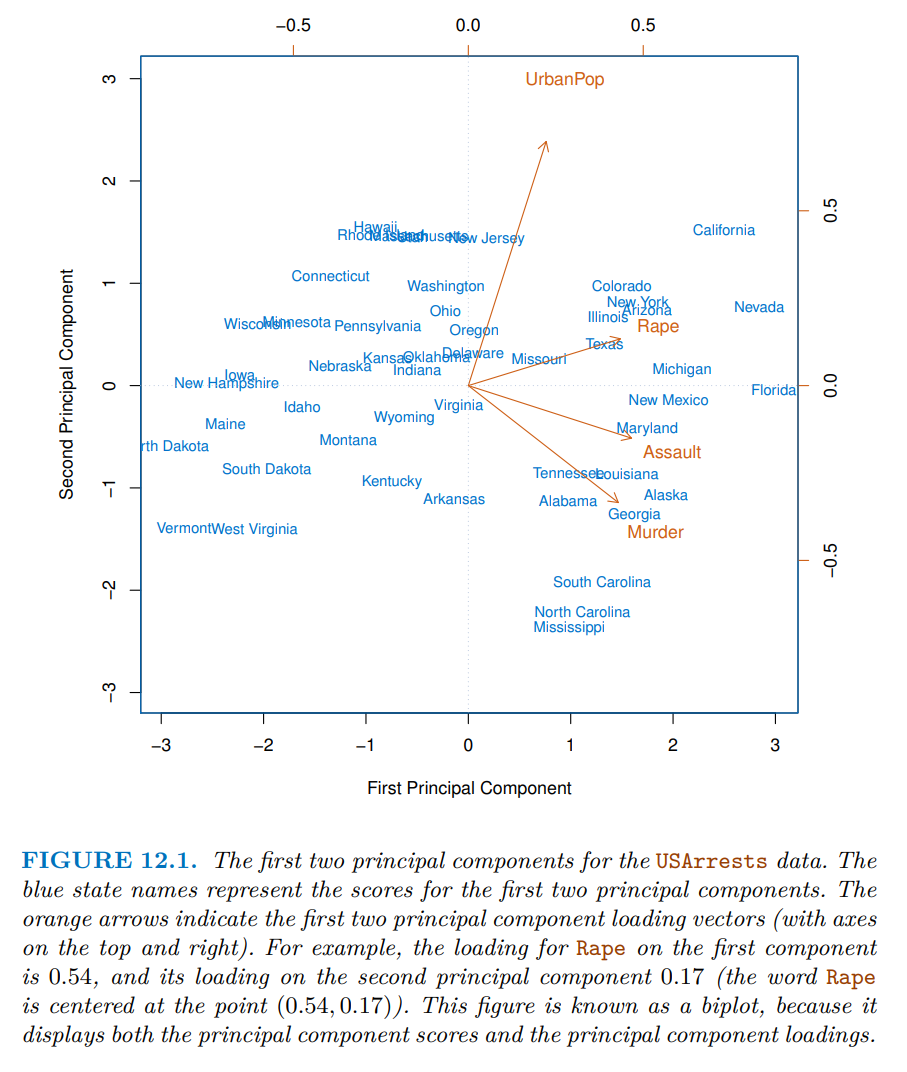
\includegraphics[width=0.7\textwidth]{Unsupervised - USArrests - Biplot.png}
    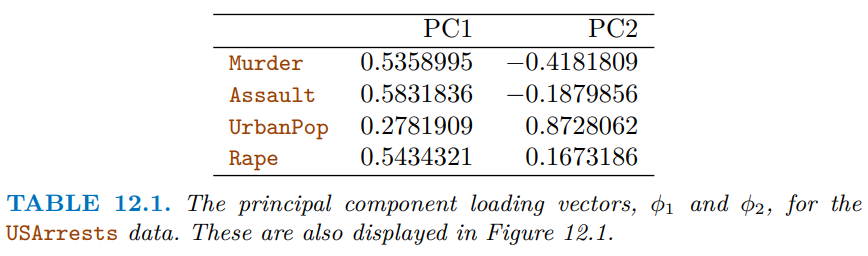
\includegraphics[width=0.7\textwidth]{Unsupervised - USArrests - Biplot Table Data.png}
\end{figure}

\noindent \textbf{Main Findings}:
\begin{itemize}
    \item In the graph, we see that the first loading vector places approximately equal weight on \textit{Assault}, \textit{Murder}, and \textit{Rape}, with must less weight on \textit{UrbanPop}. Hence this component roughly corresponds to a measure of \textbf{overall rates of serious crime}.
    \item The second loading vector places most of its weight on \textit{UrbanPop} and much less weight on the other three features. Hence, this component roughly corresponds to \textbf{the level of urbanisation of the state}.
    \item Overall, the crime-related variables are located close to each other, and that the \textit{UrbanPop} variable is far from the other three.
        \begin{itemize}
            \item This indicates that the crime-related variables are correlated with each other- states with high murder rates tend to have high assault and rape rates - and that the \textit{UrbanPop} variable is less correlated with the other three.
        \end{itemize}
\end{itemize} \phantom{i}

\noindent We can examine differences between the states via the two PC score vectors shown in the graphs.
\begin{itemize}
    \item The loading vectors suggest that \textbf{states with large positive scores on the $1$st PC}, such as California, Nevada and Florida, \textbf{have high crime rates}, while states like North Dakota, with negative scores on the $1$st PC, have low crime rates.
    \item California also has \textbf{a high score on the second component, indicating a high level of urbanisation}, while the opposite is true for states like Mississippi.
    \item \textbf{States close to zero on both components}, such as Indiana, \textbf{have approximately average levels of both crime and urbanisation}. \textit{Not a zero level}.
\end{itemize}

\subsubsection{More on PCA (Scaling, Uniqueness, PVE, and number of PCs)}
\subsubsection*{Scaling the variables}
\noindent The variables are centered to have mean zero. Furthermore, the results from PCA depend on whether the variables have been individually scaled (as they are all multiped by a different constant).\\

\noindent E.g. in the example before the variables have different units: the crimes are the number of occurrences per $100,000$ people, and \textit{UrbanPop} is the percentage of the state's population that lives in that area. The four variables have variance \textit{Murder}: $18.67$, \textit{Rape}: $87.73$, \textit{Assault}: $6945.16$, and \textit{UrbanPop}: $209.5$. \\

\noindent Consequently, if we perform PCA on the unscalaed variables, then:
\begin{itemize}
    \item $\boldsymbol{\phi_1}$ will have a very large loading for \textit{Assault};
    \item $\boldsymbol{\phi_2}$ will have a very large loading for \textit{UrbanPop}.
\end{itemize} \phantom{i}

\noindent We typically scale each variable to have s.d. of $1$ before we perform PCA. In certain settings, if the variables are the same units, then we may not wish to scale the variables.
\begin{figure}[H]
    \centering
    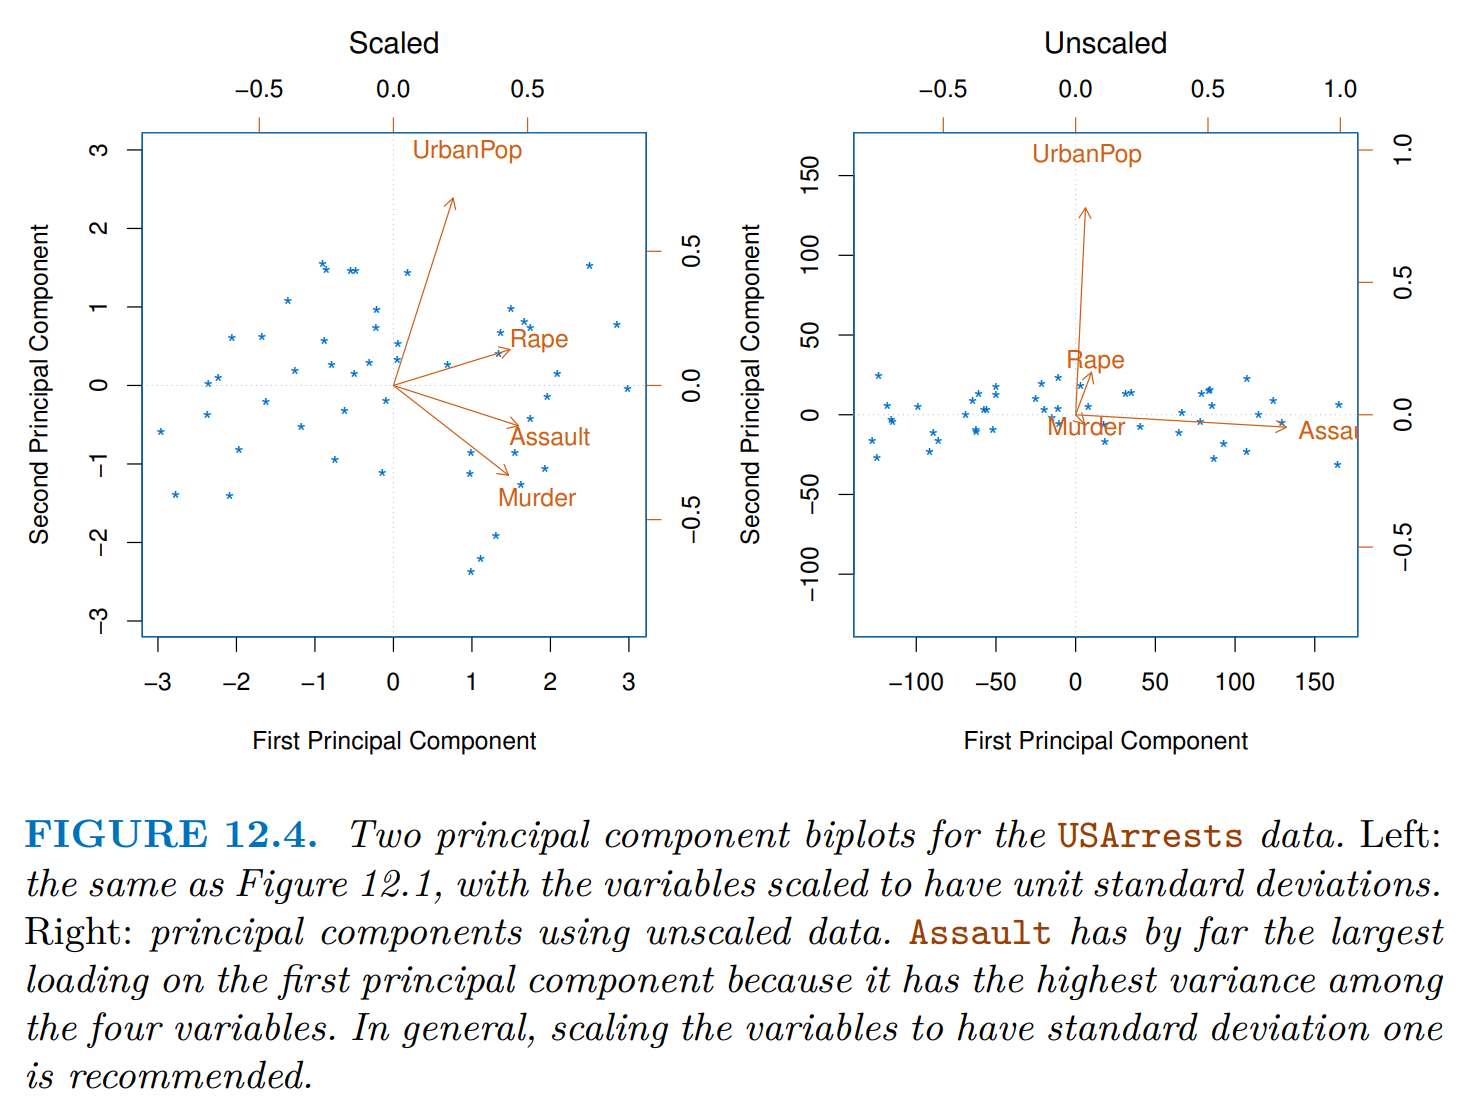
\includegraphics[width=0.6\linewidth]{Unsupervised - USArrests - Biplot Scaled vs Unscaled.png}
\end{figure}

\subsubsection*{Uniqueness of the PCs}
\noindent Each PC loading vector in unique, \textit{up to a sign flip}. Meaning you can get the same PC loading vector, although the sign of those loading vectors may differ. \\

\noindent The signs may differ because each PC loading vector specifies a direction in $p$-dimensional space: flipping the sign has no effect as the direction does not change. \\

\noindent Similarly, the score vector are unique up to a sign flip. Since the variance of $Z$ is the same as the variance of $-Z$.

\subsubsection*{Proportion of Variance Explained (PVE)}
\noindent We are usually interested in PVE by each PC. The total variance present in the data (assuming all variables have mean centered at zero) is defined as:
$$\sum_{j=1}^p{\text{Var}(X_j)} = \sum_{j=1}^{p}{\frac{1}{n}\sum_{i=1}^{n}{x_{ij}^2}}$$
\noindent and the variance explained by $Z_m$ is:
$$\frac{1}{n}\sum_{i=1}^{n}{z_{im}^{2}} = \frac{1}{n}\sum_{i=1}^{n}\Big(\sum_{j=1}^{p}{\phi_{jm}x_{ij}} \Big)^2$$
\noindent Thus, the PVE of $Z_m$ is given by:
$$\frac{\frac{1}{n}\sum_{i=1}^{n}\Big( \sum_{j=1}^{p}{\phi_{jm}x_{ij}} \Big)^2}{\sum_{j=1}^{p}\frac{1}{n}\sum_{i=1}^{n}x_{ij}^2}$$

\subsubsection*{Deciding the number of PCs to use}
\noindent We would like ot use the \textbf{smallest} number of principal components required to get a \textbf{good} understanding of the data. There is no best number of PCs to use.
\begin{itemize}
    \item An \textit{ad hoc} approach: examine a \textit{scree plot} of the data and look for an \textit{elbow} in the scree plot.
\end{itemize}
\begin{figure}[H]
    \centering
    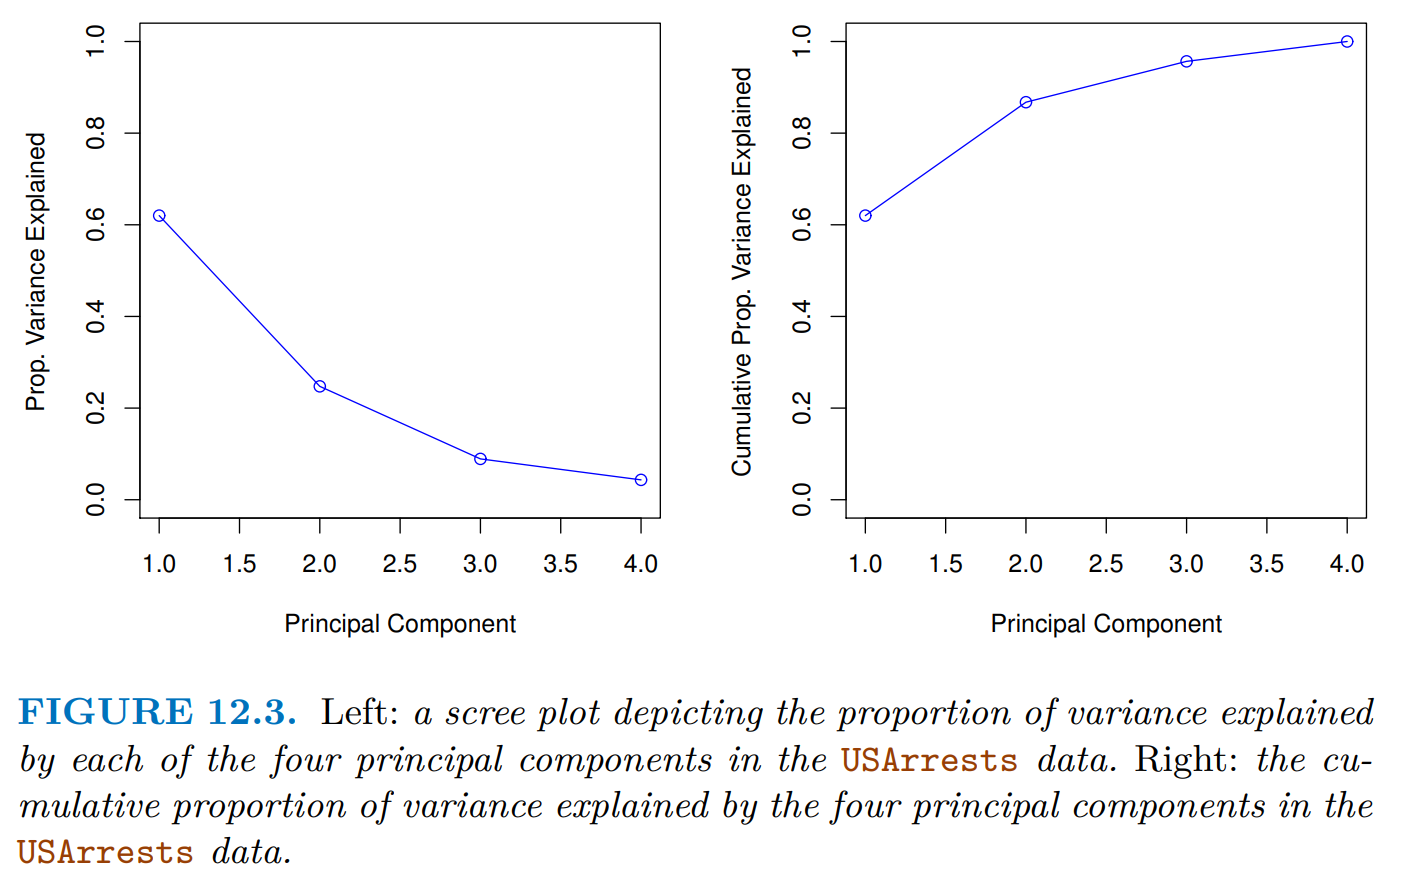
\includegraphics[width=0.7\linewidth]{Unsupervised - USArrests - Scree Plot.png}
\end{figure}
\begin{itemize}
    \item A \textit{subjective approach}: look at first few PCs in order to find interesting patterns in the data. If no interesting patterns in first few PCs, then further PCs are unlikely to be on interest. Conversely, if the first few PCs are interesting, then we typically continue to look at subsequent PCs until no further interesting patterns are found.
    \item A \textit{objective approach}: if we compute PCs for use in a supervised analysis, such as PCR, we can treat the number of PC score vectors to be used in the regression as a tuning parameter to be selected via cross-validation or a related approach.
\end{itemize}

\subsubsection{PCA in R}
\begin{lstlisting}
states=row.names(USArrests)
names(USArrests)
apply(USArrests, 2, mean) # 2 for columns
apply(USArrests, 2, var) # 2 for columns
pr.out=prcomp(USArrests, scale=TRUE) # PCA with standardisation
names(pr.out)
pr.out$center # mean of original columns
pr.out$scale # s.d. of original columns
pr.out$rotation # PC loading vectors
dim(pr.out$x) # PC scores, i.e. transformed features
biplot(pr.out, scale=0)
pr.out$rotation=-pr.out$rotation # to be consistent with textbook figure
pr.out$x=-pr.out$x
biplot(pr.out, scale=0)
pr.out$sdev # s.d. of PCs
pr.var=pr.out$sdev^2 # variance of PCs
pr.var
pve=pr.var/sum(pr.var) # calculating PVE (proportion of var explained)
pve # first 2 PCs are good enough because explain greater than 80% of the variance
plot(pve, xlab="Principal Component", ylab="Proportion of Variance Explained", 
     ylim=c(0,1),type="b") # elbow point is about 2 so good enough
plot(cumsum(pve), xlab="Principal Component",
    ylab="Cumulative Proportion of Variance Explained",
    ylim=c(0,1),type="b") # cumsum() calculates cumulative sum of elements
\end{lstlisting}

\subsection{Clustering}
\noindent We seek to partition the observations into distinct groups so that the observations within each group are homogeneous, while observations between groups are heterogeneous. \\

\noindent Clustering approaches:
\begin{itemize}
    \item \textbf{K-means clustering}: partition the observations into a pre-specified number of clusters;
    \item \textbf{Hierarchical clustering}: generate a dendrogram to visually represent the observations. Allows us to view all the clusters obtained.
\end{itemize} \phantom{i}

\noindent Two goals of clustering:
\begin{enumerate}
    \item Cluster observations on the basis of the features in order to identify \textit{subgroups among the observations}.
    \item Cluster features on the basis of the observation in order to discover \textit{subgroups among the features}.
\end{enumerate}

\subsubsection{K-means clustering}
\noindent Must first specify number of clusters $K$; then the $K$-means algorithm will assign each observation to exactly one of the $K$ clusters. \\

\noindent Let $C_1,...,C_k$ denote sets containing the indices of the observation in each cluster. These sets satisfy two properties:
\begin{enumerate}
    \item $C_1 \cup C_2 \ \cup ... \cup \ C_k = \{1,...,n\}$. In other words, each observation belongs to at least one of the $K$ clusters.
    \item $C_k \ \cup \ C_{k'} = \varnothing \; \forall k\neq k'$. The clusters are non overlapping: no observations belongs to more than one cluster.
\end{enumerate}

\subsubsection*{Idea behind K-means clustering}
\noindent A good clustering is one for which the within-cluster variation ($W(C_k)$ for cluster $C_k$) is as small as possible.
$$W(C_k) = \frac{1}{|C_k|}\sum_{i,i'\in C_k}\sum_{j=1}^{p}(x_{ij} - x_{i'j})^2 = 2\sum_{i \in C_k}\sum_{j=1}^{p}(x_{ij} - \bar{x}_{kj})^2$$.
\noindent Where $|C_k|$ denotes the number of observations in $C_k$, and $\bar{x}_{kj} = \frac{1}{|C_k|}\sum_{i \in C_k}{x_{ij}}$. \\

\noindent hence we want to solve the problem:
$$\min_{C_1,...,C_k}{\sum_{k=1}^{K}{W(C_k)}}$$
\noindent We want to partition the observations into $K$ clusters such that the total within-cluster variation, summed over all $K$ clusters, is as small as possible.  We can combine the above into one minimisation problem:
$$\min_{C_1,...,C_k}\sum_{k=1}^{K}\sum_{i \in C_k}\sum_{j=1}^{p}{(x_{ij} - \bar{x}_{kj})^2}$$

\subsubsection{K-Means clustering algorithm}
\begin{enumerate}
    \item Randomly assign a number, from $1$ to $K$, to each of the observations. These serve as initial cluster assignments for the observations, denotes $C_1^{(1)},..., C_{K}^{(1)}$. Let $I = 1$.
    \item \phantom{i}
        \begin{enumerate}
            \item For $C_{k}^{(I)}, \; k=1,...,K$, compute the cluster \textit{centroid} $\Big(\bar{x}_{k1}^{(I)}, ...., \bar{x}_{kp}^{(I)}\Big)$. i.e. the vector of the $p$ feature means for the observations in $C_{k}^{(I)}$.
            \item Assign each observation to the cluster whose centroid is closest (where teh closest is defined using Euclidean distance) to generate new clusters $C_1^{(I+1)}, ..., C_{K}^{(I+1)}$. If $C_1^{(I+1)},...,C_K^{(I+1)}$ are different from $C_1^{(1)},..., C_K^{(1)}$, then let $I = I + 1$ and repeat Step $2$; otherwise, return $C_1^{(1)},...,C_K^{(1)}$ as the output.
        \end{enumerate}
\end{enumerate} \phantom{i} \\
\noindent The algorithm can be summarised in the following flow chart:
\begin{figure}[H]
    \centering
    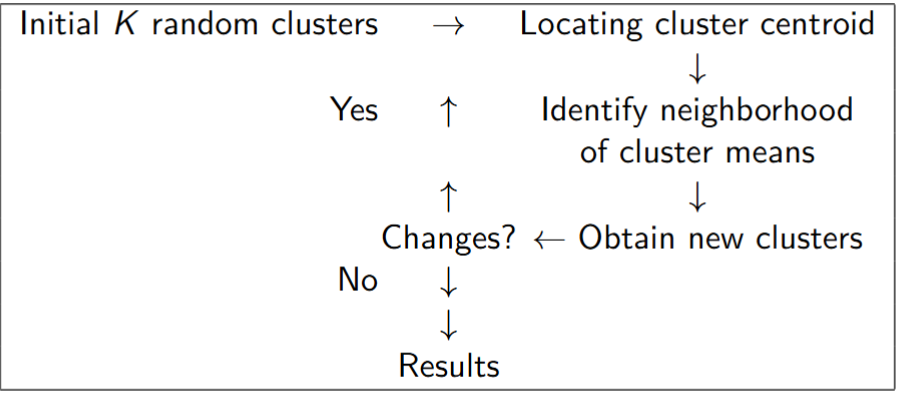
\includegraphics[width=0.7\linewidth]{K-means algorithm flow chart.png}
\end{figure}
\begin{itemize}
    \item Step 2(a) minimises the sum-of-squared deviations by updating the cluster means, $\bar{x}_{kj}, \; j=1,...,p$.
    \item Step 2(b) minimises the sum-of-squared deviations by reallocating the observations, i.e. updating $\{i \in C_k\}, \; k=1,...,K$.
    \item As we loop the algorithm, the clustering obtained will continually improve until the result no longer changes; the objective (minimisation) function will never increase.
    \item When the result no longer changes, a local optimum has been reached.
    \item The algorithm finds a local rather than a global optimum. So it depends on the initial (random) cluster obtained in step 1 of the algorithm. So its is important to run the algorithm multiple times from different random initial configurations. Then one selects the best solution, i.e. that for which the objective is the smallest.
\end{itemize} \phantom{i} \\

\noindent K-means clustering algorithm visual example:
\begin{figure}[H]
    \centering
    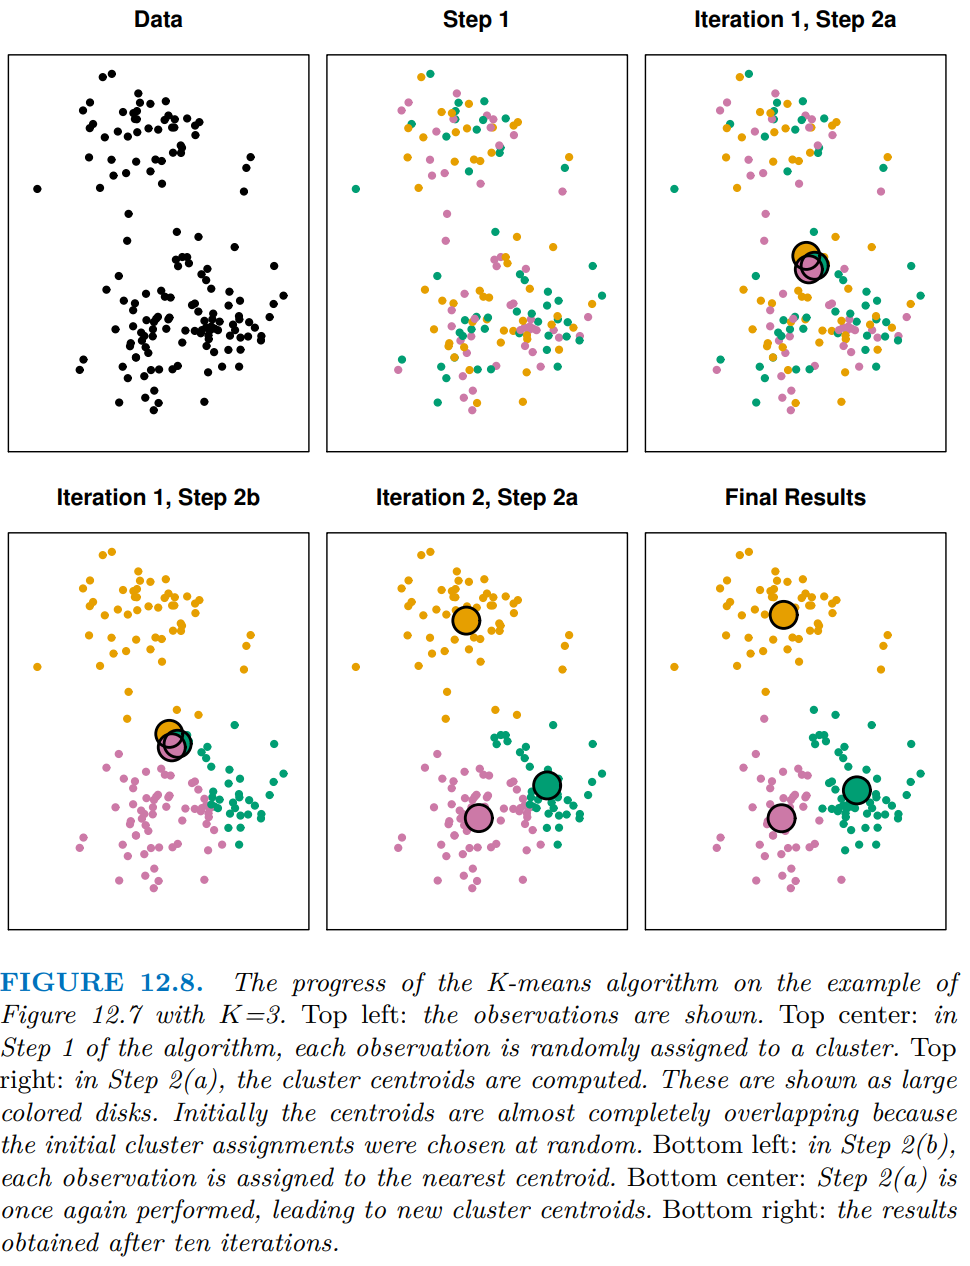
\includegraphics[width=0.5\linewidth]{K-means clusteing visual example.png}
\end{figure}

\noindent K-means clustering different initial configurations visual example:
\begin{figure}[H]
    \centering
    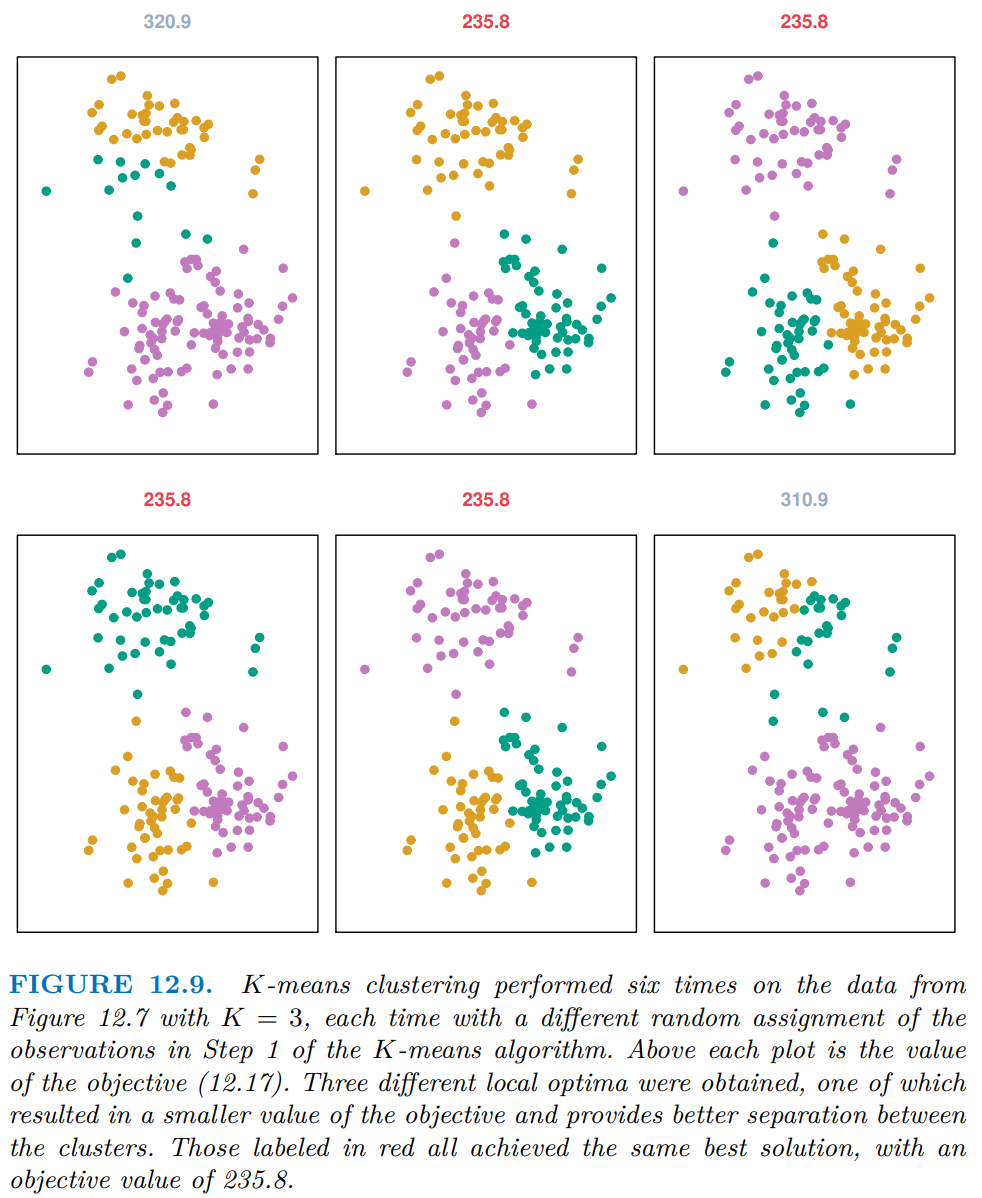
\includegraphics[width=0.5\linewidth]{K-means clustering different initial visual example.png}
\end{figure}

\subsubsection{K-means clustering in R}
\begin{lstlisting}
set.seed(2)
x=matrix(rnorm(50*2), ncol=2)
x
plot(x)
x[1:25,1]=x[1:25,1]+3
x[1:25,2]=x[1:25,2]-4
plot(x)
km.out=kmeans(x,2,nstart=20) #20 random sets were chosen and report the best one
km.out$cluster 
plot(x, col=(km.out$cluster+1), main="K-Means Clustering Results with K=2", 
     xlab="", ylab="", pch=20, cex=2)

#Try different random sets
set.seed(4)
for(i in 1:4){
km.out=kmeans(x,3,nstart=i)
print(km.out$tot.withinss)
plot(x, col=(km.out$cluster+1), main="K-Means Clustering Results with K=3", 
     xlab="", ylab="", pch=20, cex=2)
}

km.out=kmeans(x,3,nstart=20)
km.out$tot.withinss # total within cluster sum of squares
plot(x, col=(km.out$cluster+1), main="K-Means Clustering Results with K=3", 
     xlab="", ylab="", pch=20, cex=2)
\end{lstlisting}

\subsubsection{Hierarchical clustering}
\begin{itemize}
    \item Disadvantage of $K$-means clustering is that you have to pre-specify the number of clusters $K$. \textit{Hierarchical clustering does not commit to a particular choice of $K$}.
    \item Hierarchical clustering has an advantage over $K$-means is that is results in a tree based representation of the observations, a \textit{dendrogram}.
    \item \textit{Bottom-up} or \textit{agglomerative clustering} is the most common type of hierarchical clustering, and refers to the fact that the dendrogram is built starting from the leaves and combining clusters up to the trunk.
\end{itemize}

\noindent The clusters depend on what level you make the cut at in the dendrogram:
\begin{figure}[H]
    \centering
    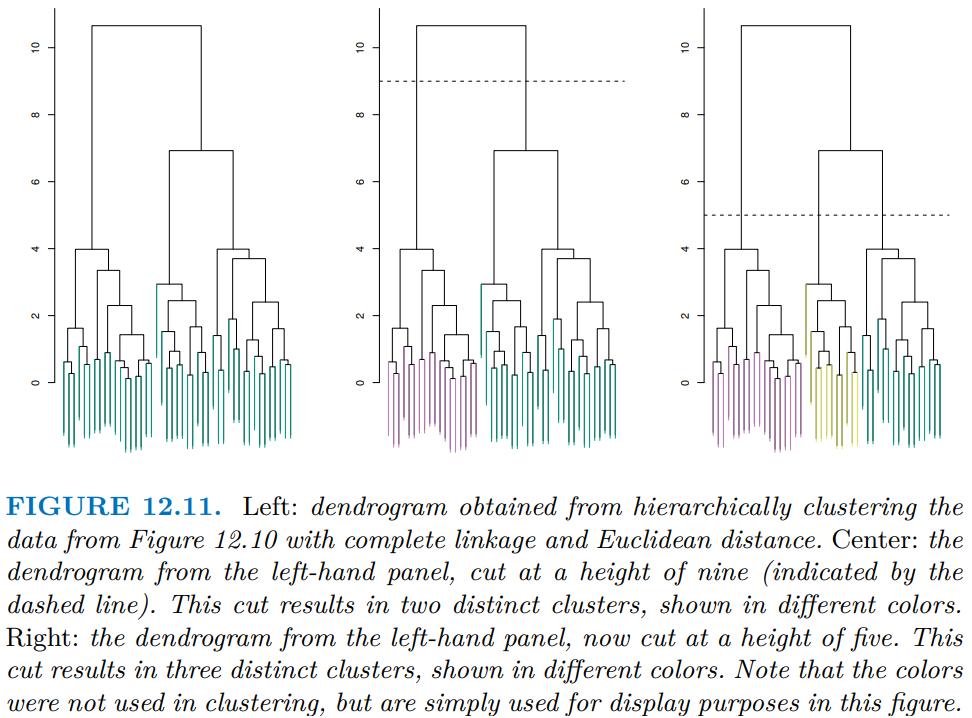
\includegraphics[width=0.7\linewidth]{Hierarchical clustering - dendrogram initial example.png}
\end{figure}

\noindent A visual example of how to interpret a dendrogram based on euclidean distance in a two-dimensional space:
\begin{figure}[H]
    \centering
    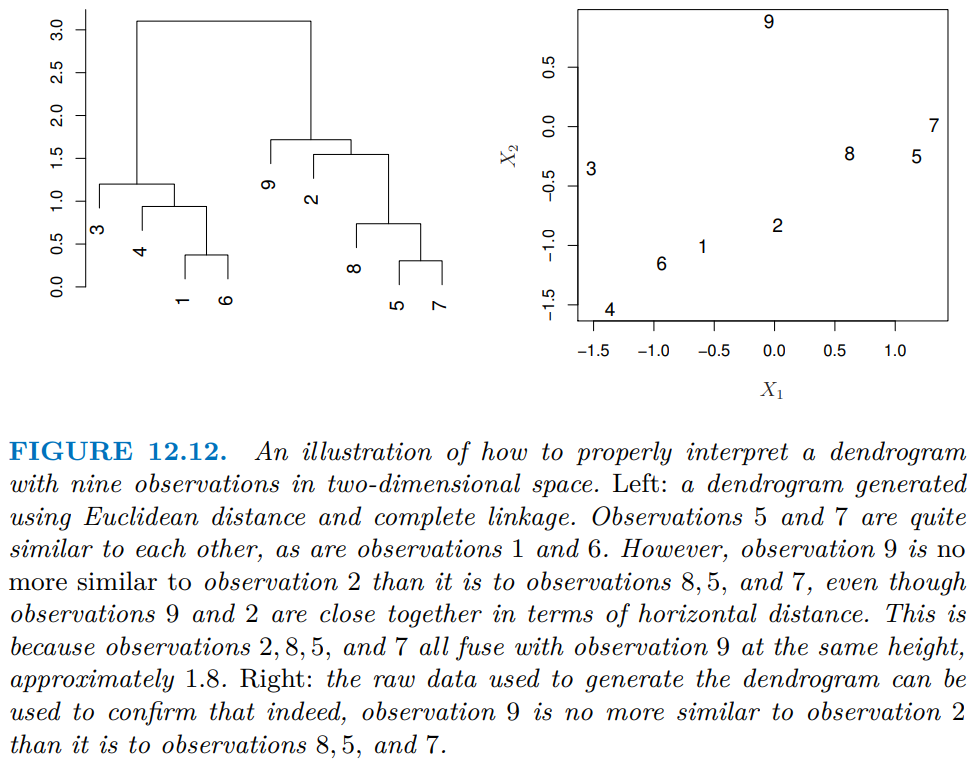
\includegraphics[width=0.7\linewidth]{Hierarchical clustering - dendrogram visual example.png}
\end{figure}

\subsubsection*{How to obtain clusters using a dendrogram}
\noindent We make a horizontal cut across the dendrogram, and the distinct sets of observations beneath the cut can be interpreted as clusters. The diagram above shows how $1$, $2$, or $3$ clusters are made in a dendrogram with different levels of cuts.

\subsubsection*{What hierarchical refers to}
\noindent The clusters obtained by cutting the dendrogam at a given height are necessarily nested within the clusters obtained by cutting the dendrogram at any greater height.

\subsubsection*{Assumption of hierarchical is unrealistic}
\noindent e.g. there is a group of people with a $50-50$ split of males and females, evenly split among Americans, Japanese, and French. In this case, the true clusters are not nested. \\

\noindent Due to situations like this, hierarchical clustering can sometimes yield worse (i.e. less accurate) results than $K$-means clustering for a given number of clusters.

\subsubsection{Hierarchical clustering algorithm}
\begin{enumerate}
    \item Being with $n$ observations and a measure (such as Euclidean distance) of all the $\binom{n}{2} = n(n-1)/2$ pairwise dissimilarities. Treat each observation as its own cluster.
    \item For $i = n,n-1,...,2$:
        \begin{enumerate}
            \item Examine all pairwise inter-cluster dissimilarities among the $i$ clusters and identify the pair of clusters that are least dissimilar (most similar). Fuse these two clusters. The dissimilarity between these two clusters indicate the height in the dendrogram at which the fusion should be placed.
            \item Compute the new pairwise inter-cluster dissimilarities among the $i-1$ remaining clusters.
        \end{enumerate}
\end{enumerate} \phantom{i} \\

\noindent An illustrating example of a dendrogram continued:
\begin{figure}[H]
    \centering
    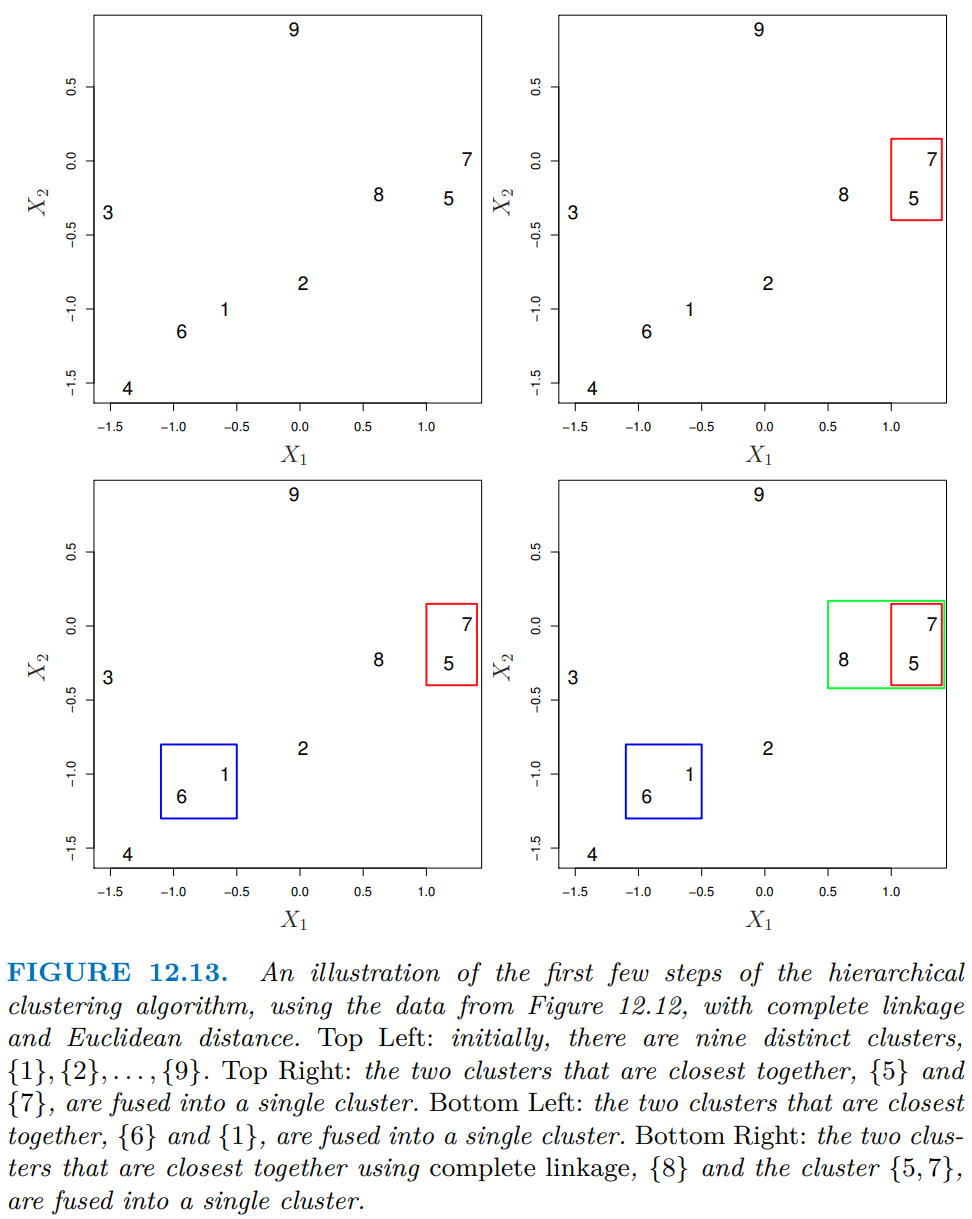
\includegraphics[width=0.7\linewidth]{Hierarchical clustering - algorithm dendrogram example.png}
\end{figure}

\subsubsection*{Dissimilarity between two clusters}
\noindent One issue with the algorithm. How do we define the dissimilarity between two clusters if one or both of the clusters contains multiple observations? The concept of dissimilarity between a pair of observations needs to be extended to a pair of groups of observations. \\

\noindent This extension is achieved by developing the notion of \textit{linkage}, which defines the dissimilarity between two groups of observations.

\subsubsection*{Most common used types of linkage}
\noindent \textit{Centroid is not assessable}
\begin{figure}[H]
    \centering
    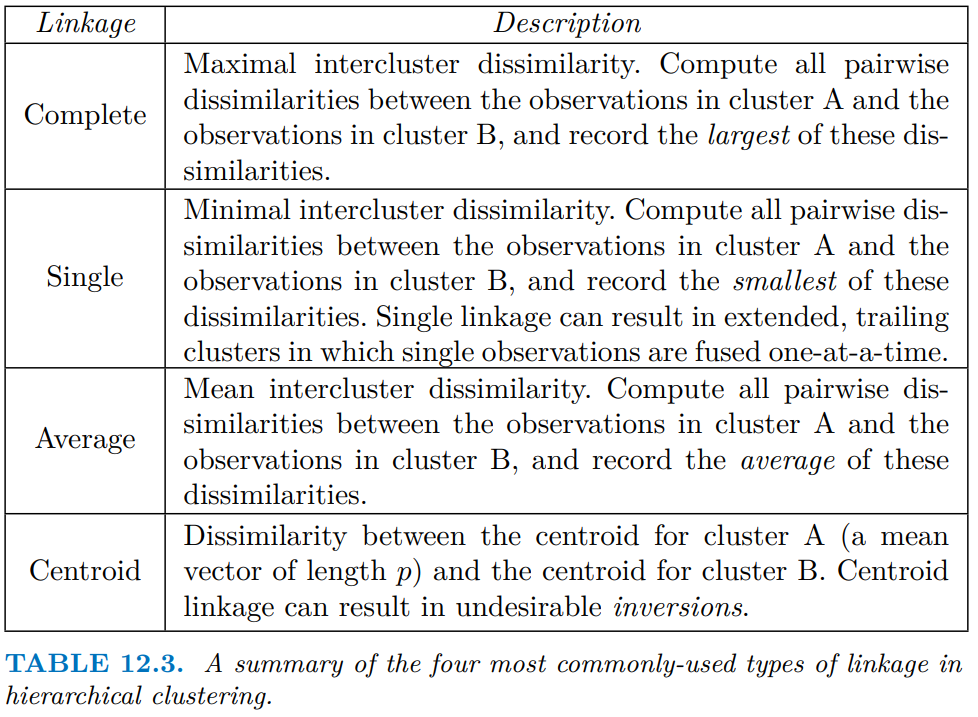
\includegraphics[width=0.7\linewidth]{Hierarchical clustering - types of linkage.png}
\end{figure}

\noindent Clustering by different types of linkage
\begin{figure}[H]
    \centering
    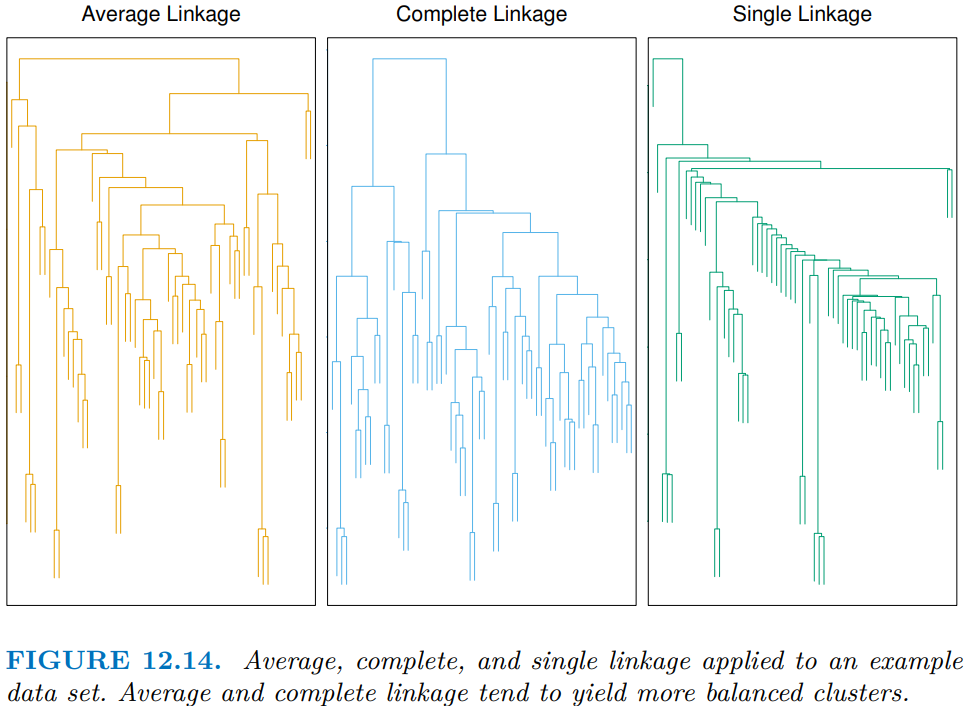
\includegraphics[width=0.7\linewidth]{Hierarchical clustering - visualisation of linkage.png}
\end{figure}

\subsubsection*{Choice of dissimilarity measure}
\noindent Apart from \textit{Euclidean} distance as the measure, we might prefer other measurer. \\

\noindent \textit{Correlation-based} distance considers two observations to be similar if their features are highly correlated, even though the observed values may be far apart in terms of Euclidean distance. \textit{correlation-based distance focuses on the shapes of observation profiles rather than their magnitudes}. \\

\noindent The choice of the dissimilarity measure has a strong effect on the resulting dendrogram. In general, \textit{careful attention should be paid to the type of data being clustered and the scientific question at hand}. The considerations should determine what type of measure is suitable.

\subsubsection*{Another example - choosing dissimilarity measure and scaling}
\noindent An online retailer interested in clustering shoppers based on their histories. The goal is to identify subgroups of similar shoppers, so that shoppers within each subgroup can be shown items and advertisements that are particular likely to interest them. \\

\noindent Assume the data takes the form of a matrix where the rows are the shoppers and the columns are the items available for purchase; the elements of the data matrix indicate the number of times a given shopper has purchased a given item (i.e. $0$ if they have never purchased it, $1$ if the shopper purchased it once, etc.) \\

\noindent \textbf{Q1: what type of dissimilarity measure should be used to cluster the shoppers}?
\begin{itemize}
    \item If Euclidean distance is used, then the shoppers who have bought very few items overall (i.e. infrequent users) will be clustered together. This may not be desirable.
    \item If correlation-based distance is used, then shoppers with similar preferences will be clustered together, even is some shoppers with these preferences are higher-volume shoppers than others.
    \item Therefore, for this application, correlation-based distance may be a better choice.
\end{itemize} \phantom{i}

\noindent \textbf{Q2: whether or not the variables should be scaled to have s.d. of one before the dissimilarity between the observations is computed}?
\begin{itemize}
    \item Some items may be purchased more frequently than others (e.g. sock to a computer).
    \item High-frequently purchases like socks therefore tend to have a much larger effect on the inter-shopper dissimilarities, and hence on the clustering ultimately obtained, than a rare purchase like computers. This may not be desirable.
    \item If the variables are scaled to have unit s.d. before the inter-observation dissimilarities are computed, then each variable will in effect be given equal importance in the hierarchical clustering performed.
    \item We might also want to scale the variables to have one s.d. if they are measured on different scales (e.g. centimeters vs kilometers).
    \item \textit{The answer to the question depends on the application at hand}.
\end{itemize}

\subsubsection{Hierarchical clustering in R}
\begin{lstlisting}
hc.complete=hclust(dist(x), method="complete")
hc.average=hclust(dist(x), method="average")
hc.single=hclust(dist(x), method="single")
par(mfrow=c(1,3))
plot(hc.complete,main="Complete Linkage", xlab="", sub="", cex=.9)
plot(hc.average, main="Average Linkage", xlab="", sub="", cex=.9)
plot(hc.single, main="Single Linkage", xlab="", sub="", cex=.9)
cutree(hc.complete, 2)
cutree(hc.average, 2)
cutree(hc.single, 2)
cutree(hc.single, 4)

xsc=scale(x) #Scaling the variables beforehand

plot(hclust(dist(xsc), method="complete"), 
     main="Hierarchical Clustering with Scaled Features")

x=matrix(rnorm(30*3), ncol=3)
dd=as.dist(1-cor(t(x))) # use 1-correlation as the distance function
plot(hclust(dd, method="complete"), 
     main="Complete Linkage with Correlation-Based Distance", xlab="", sub="")

x[,1]=x[,1]*2
x[,3]=x[,3]+5
plot(hclust(dd, method="complete"), 
     main="Complete Linkage with Correlation-Based Distance", xlab="", sub="")
# So scales have no impact if we use correlation type of distance function.

plot(hclust(dist(x), method="complete"), 
     main="Complete Linkage with U Distance", xlab="", sub="")
\end{lstlisting}

\subsubsection{Practical issues in clustering}
\begin{enumerate}
    \item \textit{Small Decisions with Big Consequences}: Each of the following decisions can have a strong impact on the results obtained. In practice, we try several choices and choose the one with the most useful solution.
        \begin{itemize}
            \item Should the observations or features first be standardised in some way?
            \item In the case of hierarchical clustering,
                \begin{itemize}
                    \item What dissimilarity measure should be used?
                    \item What type of linkage should be used?
                    \item Where should we cut the dendrogam in order to obtain clusters?
                \end{itemize}
            \item In the case of $K$-means clustering, how many clusters should we look for in the data?
        \end{itemize}
    \item \textit{Validating the Clusters Obtained}: Any time clustering is performed we will find clusters. But we really want to know whether the clusters that have been found represent true subgroups in the data, or whether they are simply a result of \textit{clustering the noise}.
        \begin{itemize}
            \item There exist a number of techniques for assignment a $p$-value to a cluster in order to assess whether there is more evidence for the cluster than one would expect due to change. However, there is no consensus on a single best approach.
        \end{itemize}
    \item \textit{Other Considerations in Clustering}: both $K$-means and hierarchical clustering will assign each observation to a cluster. However, sometimes this might not be appropriate due to the existence of outliers. Mixture models are an attractive approach for accommodating the presence of such outliers (models not need to be known for this subject).
\end{enumerate}

\subsubsection{Unsupervised learning methods example (NCI60 data) in R}
\begin{lstlisting}
library(ISLR)
nci.labs=NCI60$labs
nci.data=NCI60$data
dim(nci.data)
#View(nci.data)
nci.labs[1:4]
table(nci.labs)

# PCA on the NCI60 Data

pr.out=prcomp(nci.data, scale=TRUE)

#The function will be used to assign a color to each of the 64 cell lines, 
# based on the cancer type to which it corresponds.

Cols=function(vec){
  cols=rainbow(length(unique(vec)))
  return(cols[as.numeric(as.factor(vec))])
}
par(mfrow=c(1,2))
plot(pr.out$x[,1:2], col=Cols(nci.labs), pch=19,xlab="Z1",ylab="Z2")
plot(pr.out$x[,c(1,3)], col=Cols(nci.labs), pch=19,xlab="Z1",ylab="Z3")
summary(pr.out)
plot(pr.out)

# plot the PVE and cumulative PVE

pve=100*pr.out$sdev^2/sum(pr.out$sdev^2)
par(mfrow=c(1,2))
plot(pve,  type="o", ylab="PVE", xlab="Principal Component", col="blue")
plot(cumsum(pve), type="o", ylab="Cumulative PVE", xlab="Principal Component", col="brown3")

# Clustering the Observations of the NCI60 Data

sd.data=scale(nci.data)
par(mfrow=c(3,1))
data.dist=dist(sd.data)
plot(hclust(data.dist), labels=nci.labs, main="Complete Linkage", 
     xlab="", sub="",ylab="")
plot(hclust(data.dist, method="average"), labels=nci.labs, 
     main="Average Linkage", xlab="", sub="",ylab="")
plot(hclust(data.dist, method="single"), labels=nci.labs,  
     main="Single Linkage", xlab="", sub="",ylab="")

par(mfrow=c(1,1))
plot(hclust(data.dist, method="single"), labels=nci.labs,  
     main="Single Linkage", xlab="", sub="",ylab="")

hc.out=hclust(dist(sd.data)) #default is Complete linkage
hc.clusters=cutree(hc.out,4)
table(hc.clusters,nci.labs)
par(mfrow=c(1,1))
plot(hc.out, labels=nci.labs)
abline(h=139, col="red")
hc.out

#Try the K-means clustering with K=4

set.seed(2)
km.out=kmeans(sd.data, 4, nstart=20)
km.clusters=km.out$cluster
table(km.clusters,hc.clusters)

#Hclusering on PCs

hc.out=hclust(dist(pr.out$x[,1:5]))
plot(hc.out, labels=nci.labs, main="Hier. Clust. on First Five Score Vectors")
table(cutree(hc.out,4), nci.labs)
\end{lstlisting}

\newpage
\section{Textbook Questions Solutions}
\subsection{Linear Regression - Chpt 3}
\subsubsection{Question 8 - simple linear regression model analysis}
\subsubsection*{Part a}
\textit{Use the $lm()$ function to perform a simple linear regression with
mpg as the response and horsepower as the predictor. Use the
$summary()$ function to print the results. Comment on the output.
For example:}
\begin{lstlisting}
library(ISLR)
Auto <- na.omit(Auto)
attach(Auto)
lm.fit <- lm(mpg ~ horsepower, data=Auto)
summary(lm.fit)
\end{lstlisting}
\subsubsection*{Part i}
\textit{Is there a relationship between the predictor and the response?} \\
\noindent Yes, the $F$-statistic p-value is close to zero so we can reject the null hypothesis and state there is a statistically significant relationship between $horsepower$ and $mpg$.
\subsubsection*{Part ii}
\textit{How strong is the relationship between the predictor and the response?} \\
\noindent Since the $p$-value is extremely small, the relationship is very strong.
\subsubsection*{Part iii}
\textit{Is the relationship between the predictor and the response positive or negative?} \\
\noindent $\hat\beta_1=-0.15$, so the relationship is negative.
\subsubsection*{Part iv}
\textit{What is the predicted $mpg$ associated with a $horsepower$ of
$98$? What are the associated $95\%$ confidence and prediction
intervals?}
\begin{lstlisting}
predict(lm.fit, data.frame(horsepower=98), interval="confidence")
predict(lm.fit, data.frame(horsepower=98), interval="prediction)
\end{lstlisting}
\subsubsection*{Part b}
\textit{Plot the response and the predictor. Use the $abline()$ function to display the least squares regression line.}
\begin{lstlisting}
plot(horsepower, mpg)
abline(lm.fit)
\end{lstlisting}
\subsubsection*{Part c}
\textit{Use the $plot()$ function to produce diagnostic plots of the least
squares regression ft. Comment on any problems you see with
the ft.}
\begin{lstlisting}
par(mfrow=c(2,2))
plot(lm.fit)
\end{lstlisting}
\noindent Based on the residuals plots, there is some evidence of non-linearity.

\subsubsection{Question 9 - multiple linear regression on dataset}
\subsubsection*{Part a}
\textit{Produce a scatter plot matrix which includes all of the variables in the data set.}
\begin{lstlisting}
pairs(Auto)
\end{lstlisting}
\subsubsection*{Part b}
\textit{Compute the matrix of correlations between the variables using the function $cor()$. You will need to exclude the $name$ variable, which is qualitative.}
\begin{lstlisting}
cor(subset(Auto, select=-name))
\end{lstlisting}
\subsubsection*{Part c}
\textit{Use the $lm()$ function to perform a multiple linear regression with $mpg$ as the response and all other variables except $name$ as the predictors. Use the $summary()$ function to print the results. Comment on the output. For instance:}
\begin{lstlisting}
lm.fit1 <- lm(mpg ~ . - name, data=Auto)
summary(lm.fit1)
\end{lstlisting}
\subsubsection*{Part i}
\textit{Is there a relationship between the predictors and the response?} \\
Yes, $F$-statistic $p$-value is basically $0$, indicated evidence against the null-hypothesis. So there is a relationship.
\subsubsection*{Part ii}
\textit{Which predictors appear to have a statistically significant relationship to the response?} \\
Looking at the $p$-values of each predictors $t$-statistic. Displacement, weight, year, and origin have statistically significant relationship.
\subsubsection*{Part iii}
\textit{What does the coefficient for the $year$ variable suggest?} \\
Coefficient is $0.75$, suggesting that cars with later model years have higher $mpg$.
\subsubsection*{Part d}
\textit{Use the $plot()$ function to produce diagnostic plots of the linear regression ft. Comment on any problems you see with the ft. Do the residual plots suggest any unusually large outliers? Does the leverage plot identify any observations with unusually high leverage?}
\begin{lstlisting}
par(mfrow=c(2,2))
plot(lm.fit1)
\end{lstlisting}
Based on the diagnostic plots one can see that the data is clearly non-linear. There is also a data point (the $14$th) that has high leverage.
\subsubsection*{Part e}
\textit{Use the $*$ and $:$ symbols to ft linear regression models with interaction effects. Do any interactions appear to be statistically significant?}
\begin{lstlisting}
lm.fit2 <- lm(mpg~displacement+weight+year+origin, data=Auto)
lm.fit3 <- lm(mpg~displacement+weight+year+origin+year:origin, data=Auto)
lm.fit4 <- lm(mpg~displacement+origin+year*weight, data=Auto)
lm.fit5 <- lm(mpg~year+origin+displacement*weight, data=Auto)
summary(lm.fit2) # could get summary of rest of the models as well
\end{lstlisting}
All interaction terms seem to be statistically significant
\subsubsection*{Part f}
\textit{Try a few different transformations of the variables, such as $\log(X), \sqrt{X}, X^2$. Comment on your findings.}
\begin{lstlisting}
lm.fit6 <- lm(mpg~poly(displacement,3)+weight+year+origin, data=Auto)
lm.fit7 <- lm(mpg~displacement+I(log(weight))+year+origin, data=Auto)
lm.fit8 <- lm(mpg~displacement+I(weight^2)+year+origin, data=Auto)
summary(lm.fit6) # could get summary of the rest of the models as well
\end{lstlisting}
$\log(weight)$, $\sqrt{horsepower}$, and $acceleration^2$ all have statistical significance of some sort. The residuals plot has less of a discernible pattern than the plot of all linear regression terms. The studentized residuals displays potential outliers ($>$3). The leverage plot indicates more than three points with high leverage. \\

\noindent However, 2 problems are observed from the above plots: 1) the residuals vs fitted plot indicates heteroskedasticity (unconstant variance over mean) in the model. 2) The Q-Q plot indicates somewhat unnormality of the residuals. \\

\noindent So, a better transformation need to be applied to our model. From the correlation matrix in 9a., displacement, horsepower and weight show a similar nonlinear pattern against our response mpg. This nonlinear pattern is very close to a log form. So in the next attempt, we use log(mpg) as our response variable. \\

\noindent The outputs show that $\log$ transform of mpg yield better model fitting (better $R^2$, normality of residuals).

\subsection{Resampling Methods - Chpt 5}
\subsubsection{Question 2 - probabilities with bootstrap}

\newpage
\appendix
\section{Appendix: Summary of Statistical Learning Models}
\begin{center}
    \textbf{Refer to next page for summary.}
\end{center} \phantom{i}

\noindent Has Advantages, Disadvantages/Drawbacks, and Additional Notes for each model learnt.
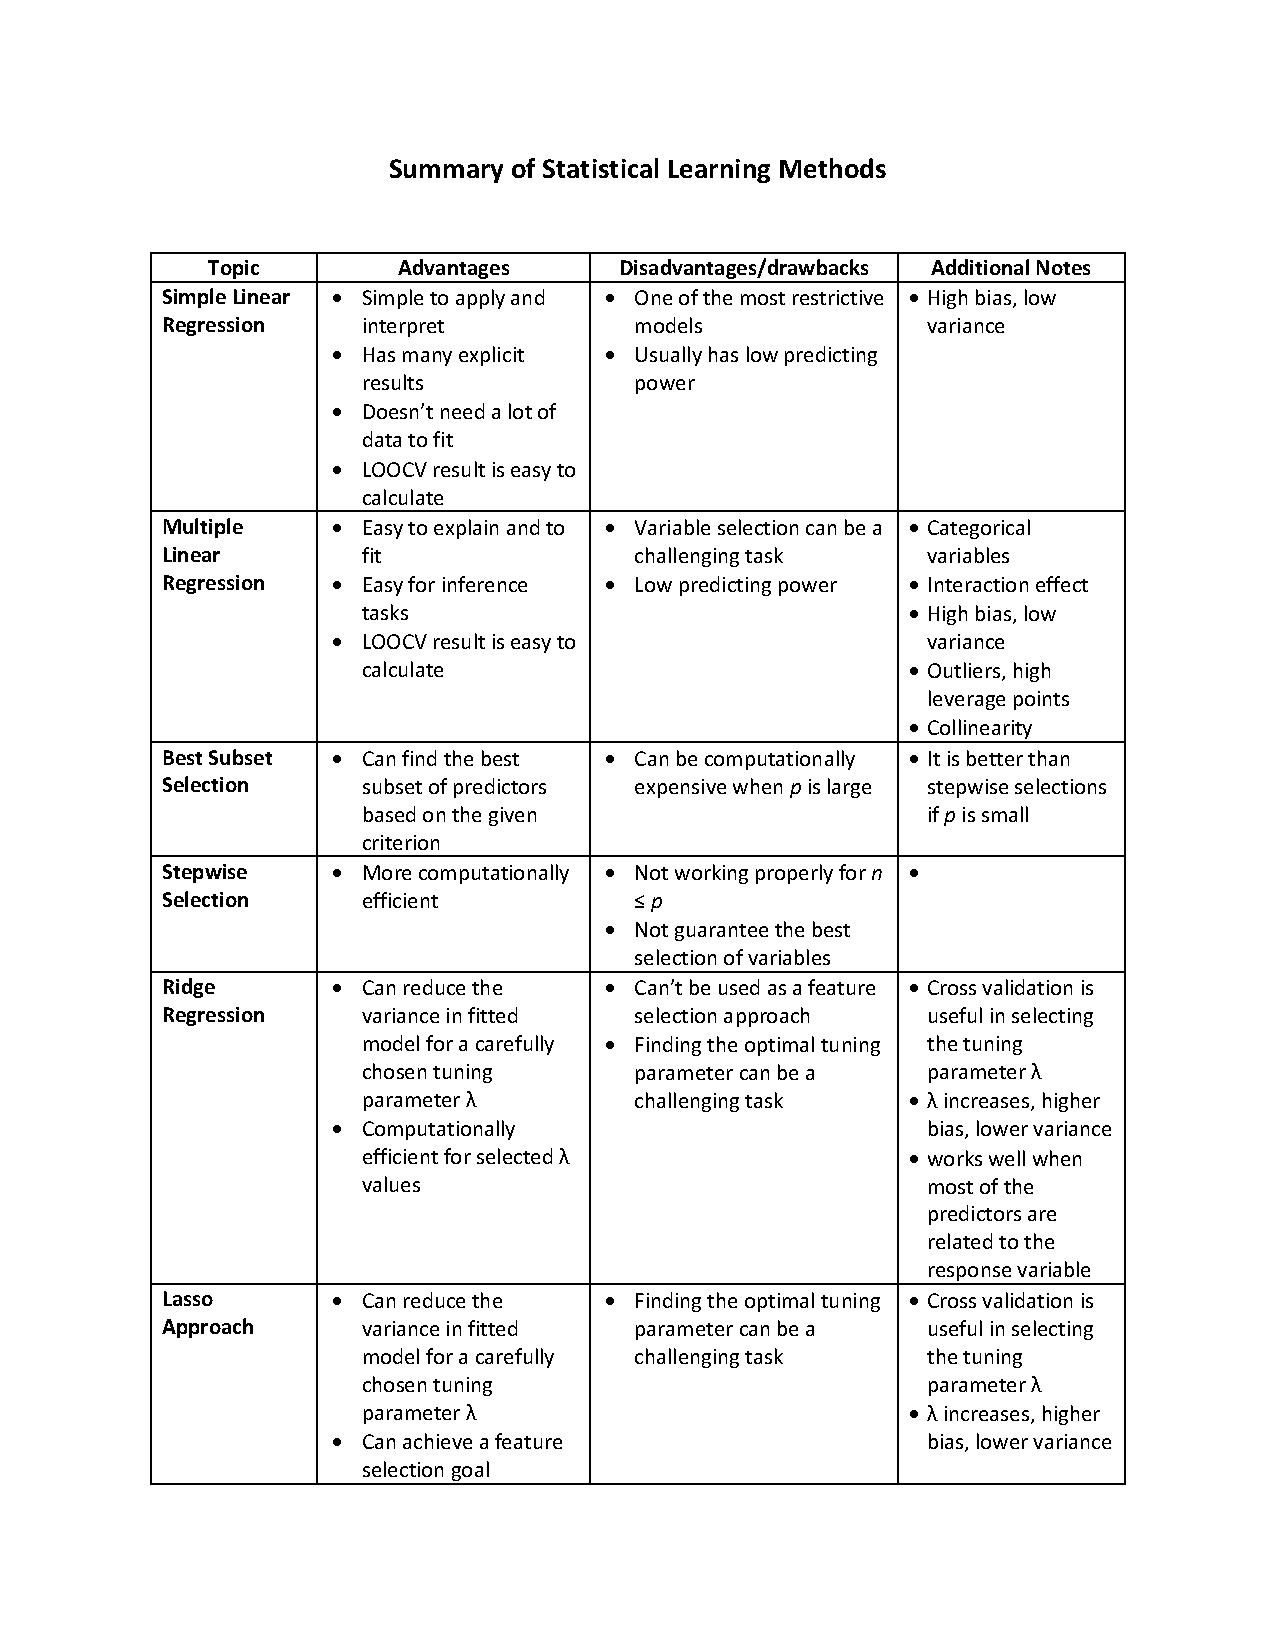
\includepdf[pages=-]{Summary of Statistical Learning Methods.pdf}

\section{Appendix: R Programming Essentials for Actuarial Data Analytics}
In this appendix, we summarize key R skills and functions that are useful for performing the analyses above in an exam setting (open-book).

\subsection{Basic Data Operations}
\begin{itemize}
    \item \textbf{Reading data:} \verb|read.table("file.txt", header=TRUE)| or \verb|read.csv("file.csv")| to import data. If the exam provides data as a CSV, use \texttt{read.csv}. The \texttt{header} argument indicates if the first row has column names.
    
    \item \textbf{Viewing data:} \verb|head(data)| (first 6 rows), \verb|dim(data)| (dimensions, i.e., number of rows and columns), \verb|names(data)| (column names), \verb|str(data)| (structure of the data frame).
    
    \item \textbf{Subsetting:} Use \verb|data[rows, cols]|. You can use numeric indices, names, or logical vectors:
    \begin{itemize}
        \item \verb|data[1:5, ]| – first 5 rows, all columns.
        \item \verb|data[, c("Age","Salary")]| – select two columns by name.
        \item \verb|data[data$Age > 30, ]| – all observations with Age > 30.
        \item The \texttt{subset()} function can also be used: \\
        \verb|subset(data, Age>30 & Salary<=50000, select=c(Name, Salary))|.
    \end{itemize}
    
    \item \textbf{Creating new variables:} \verb|data$High <- ifelse(data$Sales > 8, "Yes","No")| creates a new factor column in \texttt{data} indicating High sales.
    
    \item \textbf{Factors vs numeric:} Use \verb|as.factor()| to convert a numeric vector to a factor (useful for qualitative response variables in models), and \verb|as.numeric()| to convert factors to their underlying integer codes if needed. Many modeling functions treat factors specially by creating dummy variables.
\end{itemize}

\subsection{Statistical Modeling in R}
\begin{itemize}
    \item \textbf{Linear regression:} \verb|lm(y ~ x1 + x2 + ... + xp, data=...)|. After fitting, use \verb|summary(lm_fit)| to get coefficient estimates, standard errors, $t$-values, and $R^2$. \\ Use \verb|predict(lm_fit, newdata=..., interval="confidence")| for confidence intervals on the mean prediction, or \verb|interval="prediction"| for prediction intervals on a new observation.
    
    \item \textbf{GLM (Logistic Regression):} \verb|glm(y ~ x1 + x2, data=..., family=binomial)|. Use \verb|summary(glm_fit)| to get coefficient estimates and $z$-values. To get predicted probabilities, use \verb|predict(glm_fit, type="response")|. Then convert to class labels by comparing to 0.5 or another threshold: e.g., \verb|ifelse(prob > 0.5, "Yes","No")|.
    
    \item \textbf{LDA/QDA (MASS package):} \verb|lda()| and \verb|qda()| from \texttt{MASS}. \\ Example: \verb|lda_fit <- lda(Direction ~ Lag1+Lag2, data=Smarket, subset=train)|. Predict with \verb|predict(lda_fit, newdata=test_data)| which returns a list with \texttt{class} (predicted class) and \texttt{posterior} (probabilities for each class). Construct a confusion matrix with \verb|table(predict, actual)| and get accuracy by \verb|mean(predict==actual)|.
    
    \item \textbf{KNN (class package):} Prepare matrices of predictors and factor of labels. Example:
    \begin{verbatim}
library(class)
knn_pred <- knn(train.X, test.X, train.Y, k=5)
    \end{verbatim}
    Then use \verb|table(knn_pred, test.Y)| to see the results.
    
    \item \textbf{Decision Trees (tree package):} Fit by \verb|tree_fit <- tree(Target ~ predictors, data=...)|. Plot the tree with \verb|plot(tree_fit); text(tree_fit, pretty=0)|. \texttt{pretty=0} displays category names for splits instead of numeric codes. Prune with cost-complexity:
    \begin{verbatim}
cv_tree <- cv.tree(tree_fit, FUN=prune.misclass)
prune_tree <- prune.misclass(tree_fit, best=<size>)
    \end{verbatim}
    Then plot the pruned tree. Use \verb|predict(prune_tree, newdata, type="class")| for classifications.
    
    \item \textbf{Support Vector Machine (e1071 package):} \\ \verb|svm_fit <- svm(y ~ ., data=..., kernel="radial", gamma=..., cost=..., scale=TRUE)|. \texttt{scale=TRUE} standardizes features (important if on different scales). After fitting, use \verb|predict(svm_fit, newdata)| to get classes. Use \\ \verb|tune(svm, y ~ ., data=..., ranges=list(cost=..., gamma=...))| for cross-validation to find optimal parameters.
    
    \item \textbf{PCA (prcomp in base R):} \verb|pr.out <- prcomp(mydata, scale.=TRUE)|. Then:
    \begin{itemize}
        \item \texttt{pr.out\$sdev}: standard deviations of PCs.
        \item \texttt{pr.out\$rotation}: matrix of PC loadings (each column is a principal component loading vector).
        \item \texttt{pr.out\$x}: the PC scores (each observation's coordinates in PC space).
    \end{itemize}
    To determine how many PCs to keep, compute:
    \begin{verbatim}
pr.var <- pr.out$sdev^2
pve <- pr.var / sum(pr.var)
    \end{verbatim}
    This gives proportion of variance explained by each component (PVE). You can print or plot \texttt{pve} and \texttt{cumsum(pve)}.
    
    \item \textbf{Clustering:}
    \begin{itemize}
        \item \textbf{K-means:} \verb|kmeans(scale(data), centers=K, nstart=20)|. \texttt{nstart} (number of random starts) is recommended to avoid local optima. The result has \texttt{\$cluster} (cluster assignment for each observation) and \texttt{\$centers} (cluster means).
        
        \item \textbf{Hierarchical:} Use \verb|dist()| to compute distance matrix, then \verb|hclust()| on that. Example:
        \begin{verbatim}
d <- dist(scale(mydata))
hc <- hclust(d, method="complete")
plot(hc)
cutree(hc, k=4)  # cut tree into 4 clusters
        \end{verbatim}
        You can try different linkage: \texttt{"single"}, \texttt{"average"}.
    \end{itemize}
    
    \item \textbf{Setting a seed:} Use \verb|set.seed(123)| for reproducibility (especially important for random splits in CV, initializations in k-means, etc.).
\end{itemize}

\subsection{Model Evaluation and Utility Functions}
\begin{itemize}
    \item \textbf{Cross-validation:} Use \texttt{cv.glm} for GLMs, or manual for others. E.g., for $K$-fold partition, one approach:
\begin{lstlisting}
folds <- sample(1:K, n, replace=TRUE)
cv_errors <- rep(0, K)
for(k in 1:K){
    fit <- lm(mpg ~ poly(horsepower, 2), data=Auto[folds!=k, ])
    pred <- predict(fit, Auto[folds==k, ])
    cv_errors[k] <- mean((Auto$mpg[folds==k] - pred)^2)
}
mean(cv_errors)
\end{lstlisting}
    But high-level libraries (like \texttt{caret} or functions like \texttt{tune()}) can simplify this for certain models.
    
    \item \textbf{Confusion matrix and metrics:} After obtaining predictions and actuals, use \\ \verb|table(predicted, actual)|. 

    Accuracy = 
    \[
    \frac{\text{TP} + \text{TN}}{\text{Total}} = \texttt{mean(pred==actual)}
    \]

    Sensitivity = 
    \[
    \frac{\text{TP}}{\text{TP} + \text{FN}}
    \]
    
    Specificity = 
    \[
    \frac{\text{TN}}{\text{TN} + \text{FP}}
    \]

    In R, you may calculate these manually or use the \texttt{caret::confusionMatrix()} function on factors of predictions and actuals (which reports many metrics).
    
    \item \textbf{General plotting:} 
    \subsection{R Plotting and Annotation Commands}\

\subsubsection*{General Plotting with \texttt{plot()}}
\begin{lstlisting}
plot(x, y,
    type      = "p",     % "p"=points, "l"=lines, "b"=both, "o"=overlaid,
                            % "h"=histogram-like verticals, "s"/"S"=steps
    col       = "black", % point/line color (e.g. "red", ...)
    pch       = 16,      % plotting symbol (1=empty circle, 16=solid circle)
    cex       = 1.0,     % point size multiplier
    lwd       = 1,       % line width multiplier
    lty       = 1,       % line type (1=solid, 2=dashed, 3=dotted, ...)
    xlab      = "X label",
    ylab      = "Y label",
    main      = "Title",
    sub       = "Subtitle",
    xlim      = c(xmin, xmax),
    ylim      = c(ymin, ymax),
    asp       = NA,      % aspect ratio y/x
    axes      = TRUE,    % draw axes?
    frame.plot= axes,    % draw box if axes=FALSE
    ann       = TRUE     % annotate with xlab, ylab
    )
\end{lstlisting}

\subsubsection*{\texttt{points()}, \texttt{lines()} and \texttt{abline()}}
\begin{lstlisting}
points(x2, y2,
    pch = 17, # symbol code
    col = "blue",
    cex = 1.5) # adds points to existing plot

lines(xg, yg,
    type = "l", # "l", "b", "p", "o", etc.
    col  = "red",
    lty  = 2, # dashed
    lwd  = 2) # adds lines or points+lines

abline(lm_obj,
    col = "darkgreen",
    lwd = 2) # add regression line from lm object

abline(h = y0, # horizontal line at y = y0
    col = "gray", lty = 3)}

abline(v = x0, # vertical line at x = x0
    col = "gray", lty = 3)}

abline(a = a0, b = b0, # line y = a0 + b0 * x
    col = "purple", lwd = 1.5)}
\end{lstlisting}

\subsubsection*{\texttt{text()}, \texttt{mtext()} and \texttt{legend()}}
\begin{lstlisting}
text(x, y,
    labels = row.names(df),
    pos    = 4, # 1=below,2=left,3=above,4=right
    offset = 0.5,
    col    = "darkred",
    cex    = 0.8)

mtext("Caption or source", 
    side = 1, # 1=bottom, 2=left, 3=top, 4=right
    line = 4, # margin line
    adj  = 1, # 0=left,1=right
    cex  = 0.8)}

legend("topright",
    legend = c("Observed","Fit"),
    col    = c("black","red"),
    pch    = c(16,NA),
    lty    = c(NA,1),
    lwd    = c(NA,2),
    pt.cex = c(1.2,NA),
    bty    = "n", # no box
    inset  = 0.02,
    cex    = 0.9)}
\end{lstlisting}

\subsubsection*{\texttt{par()} for Layout and Styles}
\begin{lstlisting}
par(mfrow = c(2,2)) # 2x2 plotting panels
par(mar = c(4.5,4.5,3,1)) # margins (bottom,left,top,right)
par(oma = c(1,1,1,1)) # outer margin
par(cex.lab = 1.1, # axis label size
    cex.main = 1.2, # main title size
    cex.axis = 0.9) # axis tick label size
par(las = 1) # axis labels always horizontal
\end{lstlisting}

\subsubsection*{\texttt{axis()} and \texttt{grid()}}
\begin{lstlisting}
axis(side = 1,
    at     = c(0,5,10),
    labels = c("0","5","10"),
    las    = 1,
    cex.axis = 0.8)}

grid(nx = NULL, ny = NULL,
    col = "lightgray",
    lty = "dotted",
    lwd = 1) # add background grid
\end{lstlisting}

    \begin{itemize}
        \item Scatterplot: \verb|plot(x, y)|. Use \verb|col| to color points (can map classes to colors), \verb|pch| to change point type.
        \item Add lines: \verb|abline(lm_fit)| adds a regression line; use \verb|lines(x_grid, predictions)| for non-linear fits.
        \item Multiple plots: \verb|par(mfrow=c(2,2))| to arrange 4 plots, etc.
        \item Identify points: \verb|plot(...); text(x, y, labels=row.names(data))| to label points by name or index (useful for spotting outliers on plots).
    \end{itemize}
\end{itemize}
\end{document}
